
\chapter{Breadth: Focused Design Projects}
\label{ch:applications}

%
%\begin{figure}[h] %  figure placement: here, top, bottom, or page
%   \centering
%   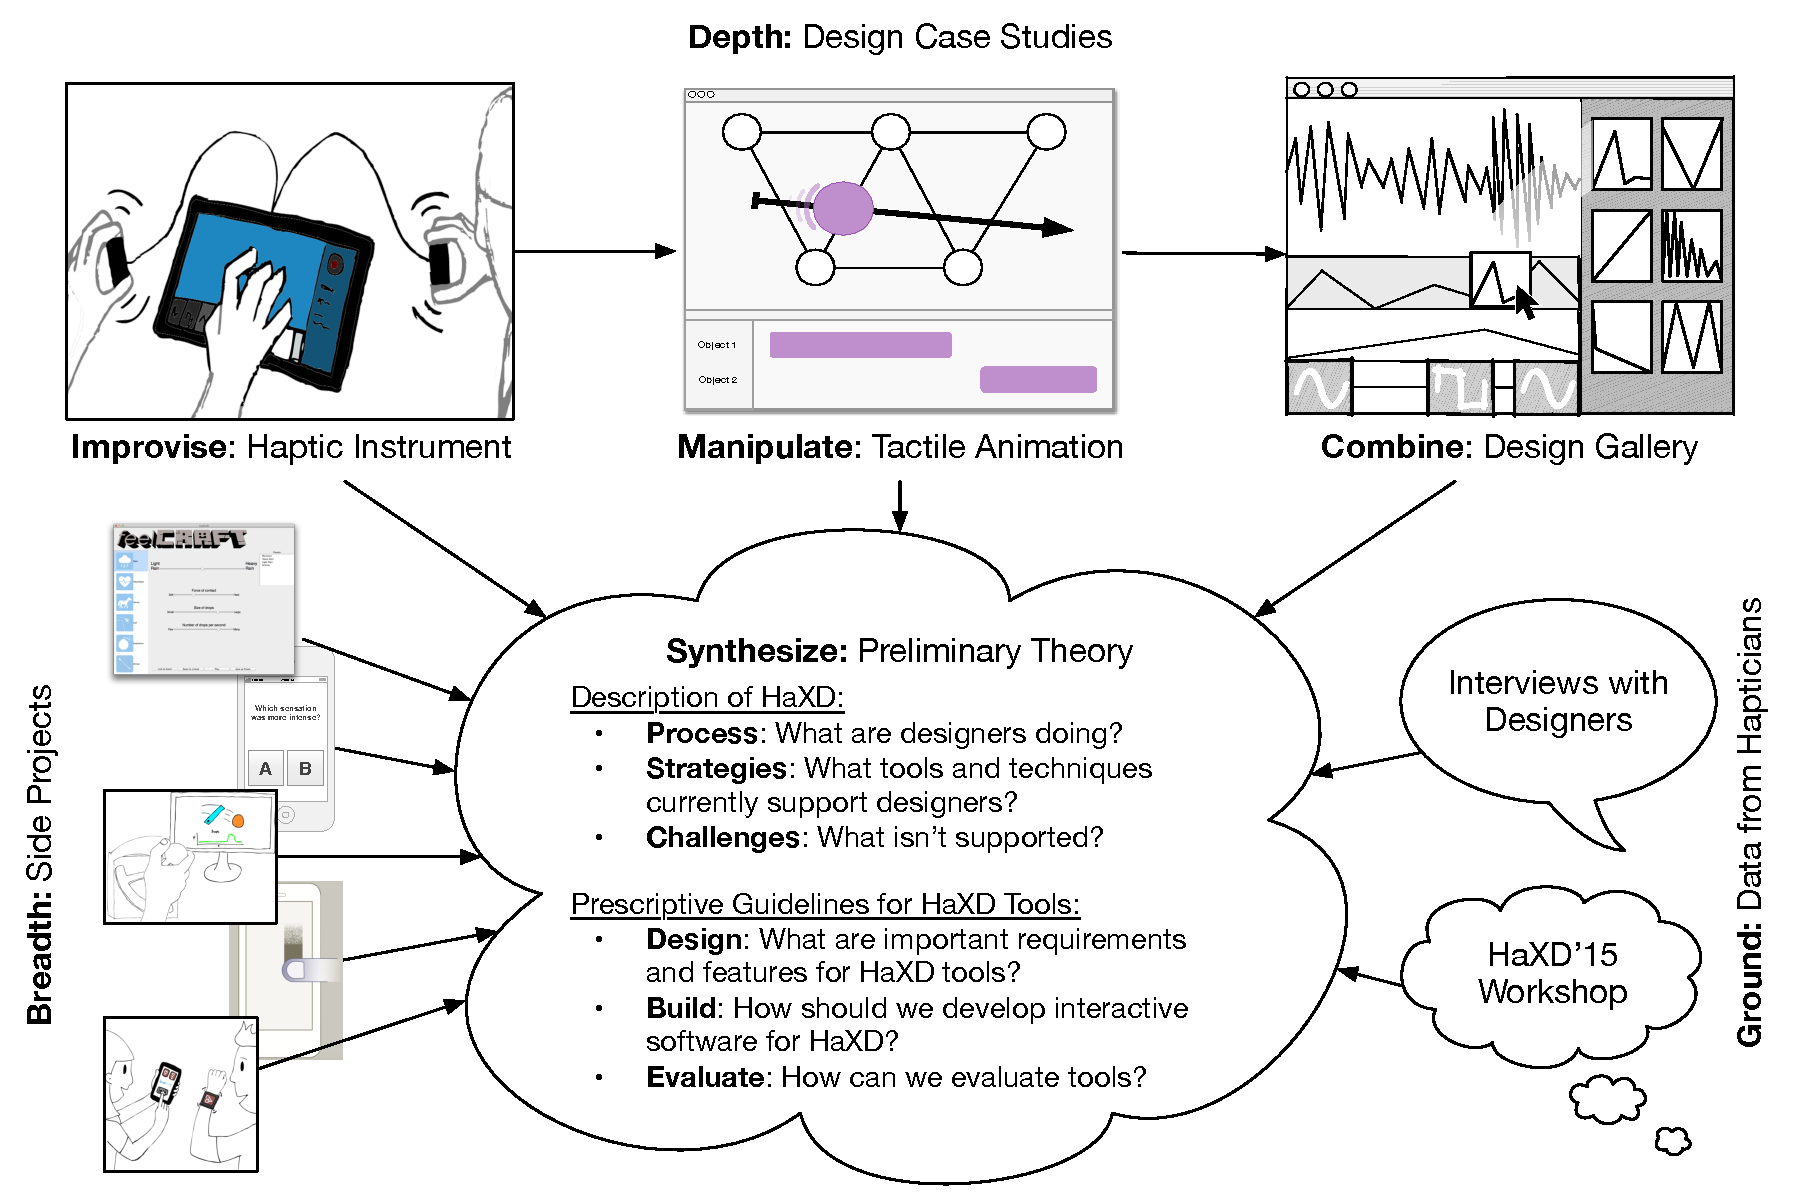
\includegraphics[width=0.7\textwidth]{HaXDTheoryOutline-2015-05-22} 
%   \caption{Planned synthesis of data for a preliminary theory of haptic experience design.}
%   \label{fig:haxd:theoryoutline}
%\end{figure}

In \autoref{ch:applications}, we complement the vibrotactile tools and techniques in Chapters \ref{ch:hapticinstrument}-\ref{ch:hapturk}, broadening 
our scope to include application areas like gaming and education, non-vibrotactile haptic devices, and \osE{other design concerns} like customization\osE{.} % and other methods of \emph{sharing}.
We adopt a haptic designer's role to gain first-hand knowledge into \haxd in a more natural design setting than our one-session lab-based evaluations.
We include five design projects:
%Chapters \ref{ch:hapticinstrument}-\ref{ch:macaron} describe provide rich provide rich but focused data on how to create vibrotactile (VT) experience design tools, and Chapter 7 provides a detailed look at a VT technique for large-scale feedback.
%To complement these studies, I participated in several more focused projects, to examine other application areas, categories of devices, and gain first-hand experience as a haptic designer:
\begin{enumerate}
    \item[\bf\ref{sec:applications:feelcraft}]
    \textbf{FeelCraft: Sharing Customized Effects for Games}\footnote{\fullCitation{SchneiderAsiaHaptics2014}}\footnote{\fullCitation{Schneider-demo-feelcraftUIST2014}}, a plug-in architecture for distributing customizable feel effects, implemented with the game Minecraft.
    
    \item[\bf\ref{sec:applications:feelmessenger}]
    \textbf{Feel Messenger: Expressive Effects with Commodity Systems}\footnote{\fullCitation{Israr2015}}\footnote{\fullCitation{Schneider-demo-feelmessenger2015}}, a design project creating expressive shareable VT icons on commodity smart phones.
    
    \item[\bf\ref{sec:applications:roughsketch}]
    \textbf{RoughSketch: Designing for an Alternative Modality}, a drawing application using programmable friction with the TPad phone.
    
    \item[\bf\ref{sec:applications:handson}]
    \textbf{HandsOn: Designing Force-Feedback for Education}\footnote{\fullCitation{Minaker2016}}, a conceptual model for DIY force-feedback haptics in education. 
    %\footnote{\inlineCitation{Martinez-demo-hapkit2016}}
    
    \item[\bf\ref{sec:applications:cuddlebit}]
    \textbf{CuddleBit Design Tools: Sketching and Refining Affective Robot Behaviours}\footnote{\fullCitation{Bucci2016}}, Voodle and MacaronBit are design tools for CuddleBits, simple affective robots.
\end{enumerate}

\noindent
\osE{Most of this chapter (Sections \ref{sec:applications:feelcraft}-\ref{sec:applications:roughsketch}) and \ref{sec:applications:cuddlebit}}  were primarily presented as demos with associated papers\osE{. As such,} we present \osE{this chapter's work} in a summary format rather than full reproduction\osE{, and exclude prefaces.}

\section{FeelCraft: Sharing Customized Effects for Games}
\label{sec:applications:feelcraft}
%In recent years, haptic feedback has shown promise to enhance user experience in movies, games, rides, virtual simulations, and social and educational media [1?3]. However, current mainstream media has yet to use the richness of haptic modality within its content. The lack of haptic authoring tools, production infrastructure,
%standardized playback protocols, and skilled and trained workers has contributed to the difficulty of integrating haptic content with accompanying media. To reduce the gap between haptics and mainstream communication, haptic feedback must be expressive, coherent, and synchronized with the content of the media, and also meet user expectations. We believe that allowing end users to access, customize, and share haptic media will create an intimate, engaging, and personalized experience, and proliferate the use of haptics.

As shown in prior work \cite{Seifi2013,Seifi2014}, and as we will discuss in \autoref{ch:hapticianinterviews}, customization is an important feature for haptic experiences.
In addition, haptic media must be built around existing infrastructure, as it is not directly supported by most media types.
FeelCraft is a media plugin architecture that monitors events and activities in the media, and associates them to user-defined haptic content in a seamless, structured way.
The FeelCraft plugin allows novice users to generate, recall, save, and share haptic content, and play and broadcast them to other users to feel the same haptic experience, without requiring any skill in haptic content generation.
In this chapter, we describe the plug-in architecture, envisioned applications, and our implementation for VT grid arrays displaying Feel Effects (FEs) \cite{Israr2014} for a popular video game, Minecraft.
Our implementations uses the Marvel Avengers Vybe Haptic Gaming Pad by Comfort Research (\url{http://comfortresearch.com}), a chair-shaped pad with 12 actuators (6 voice coils and 6 rumble motors).
We designed effects that leveraged this display, \eg, voice coils simulating rain on the user's back when there is rain in-game, and rumble motors creating a galloping sensation on the chair's seat when the user rides an virtual horse.

%In the current implementation, we concentrate on the vibrotactile array as the source of sensation and the back as the surface for stimulation; however, the FeelCraft architecture can be easily adapted for other haptic feedback modalities. We begin by presenting relevant background work related to haptic media
%infrastructure. We then present the FeelCraft architecture and describe in detail each component of the system. Finally, we conclude the paper with our envisioned application ecosystem.
%In this paper, we propose and implement an architecture that channels media
%content to dynamic and expressive tactile sensations.

%\subsection{Approach}
%Infrastructures to integrate haptic feedback in media have been primarily derived from media type and user interactions associated with the content.
%These infrastructures fall into two categories: event triggers and direct mappings.
%In the event triggers scheme, haptic information is embedded in the media and played back using predefined protocols [4?]. 
%A common example is a video game controller that rumbles on predefined triggers embedded in the games.
%This technique typically requires dedicated production infrastructure and access to tools and libraries for creating expressive haptic effects, similar to the libraries for visual and sound effects [5].
%Direct mappings use cues from existing media and directly maps them to haptic effects.
%For example, a typical way to enhance movies and other visual content with haptics is to monitor activity in a video feed [6] and map these activities to haptic transducers arranged along the seat [1, 7].
%This way, movements in a visual scene are mapped to gross motion collocated with events seen in 4D movies and rides (www.d-box.com).
%%Similarly, sound has been used to derive haptic cues for video games and music [8, 9].
%%For example, Buttkicker technology (Guitammer, USA) shakes the entire seat using low-pass filtered sound.
%%The Vybe Haptic Gaming Pad (Comfort Research) divides sound into three bands and maps them to transducers located in the seat and back. The advantage of the direct mapping scheme is that no change is required in the current media production process. However, each technique is limited to its media type.
%\osC{The above-mentioned descriptions don't really make sense.}


%\begin{itemize}
%	\item link existing and new media to the haptic feedback technology,
%	
%	\item use an FE library to find appropriate semantically defined effects,
%	
%	\item author, customize, and share a common, evolving repository of FEs, and
%	
%	\item play and broadcast haptic experiences to one or more user(s).
%\end{itemize}


\subsection{FeelCraft Plugin and Architecture}
A FeelCraft plugin maps media to haptic sensations in a modular fashion, supporting arbitrary media types and output devices.
By using a FeelCraft plugin, users can link existing and new media to the haptic feedback technology, use an FE library to find appropriate semantically defined effects, author, customize, and share a common, evolving repository of FEs, and play and broadcast haptic experiences to one or more user(s).
A pictorial description of the FeelCraft architecture is shown in Fig. 1 architecture.

The conceptual framework of FeelCraft revolves around the FE library introduced in \cite{Israr2014}.
The FE library provides a structured and semantically correct association of media events with haptic feedback.
By using the authoring interface to tailor FE parameters, a repository of FEs can remain general while being used for unique, engaging, and suitable sensations for different media.
The playback system, authoring and control interface, Event2Haptic mappings, and media plugin support seamless flow of the media content to the haptic feedback hardware.

\begin{figure}[htbp] %  figure placement: here, top, bottom, or page
   \centering
   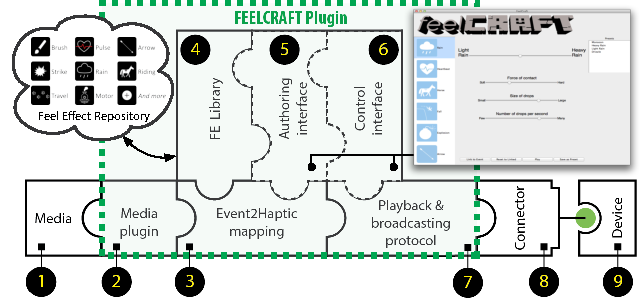
\includegraphics[width=\textwidth]{feelcraft/FeelCraftArchitecture2-2014-07-23-1805} 
   \caption{FeelCraft architecture. The FeelCraft plugin is highlighted in green. The FE library can connect to shared feel effect repositories to download or upload new FEs. A screenshot of our combined authoring and control interface is on the right.}
   \label{fig:feelcraft:architecture}
\end{figure}

\begin{description}
	\item[Media (1)] can be entertaining, such as video games, movies, and music, or
social and educational.
The media can also be general user activity or embedded events in applications. In our implementation (\autoref{fig:feelcraft:ecosystem}), we use the popular sandbox indie game Minecraft (https://minecraft.net).

	\item[Media Plugin (2)] is a software plugin that communicates with the media and
outputs events and activities. This plugin can be as simple as receiving messages from the media or as complicated as extracting events and activities from a sound stream. With existing media, common plugin systems are automatic capture of semantic content from video frames \cite{Isokoski2012}, camera angles \cite{Danieau2014}, or sounds \cite{Lee2013,Chang2005}, or the interception of input devices (such as game controllers or keyboard events). We use a CraftBukkit Minecraft server modification to capture in-game events.

	\item[Event2Haptic (3)] mappings associate events to FEs, which are designed, tuned,
and approved by users using the FE library. This critical component links the media plugin's output to the haptic playback system. Currently, six FEs are triggered by six recurring in-game events: the presence of rain, low player health, movement on horse, strike from a projectile, in-game explosions, and player falls. Our implementation provides the option to store this mapping directly in the source code, or in a text-based JavaScript Object Notation (JSON) file

	\item[FE Library (4)] is a collection of FEs. A key feature of an FE is that it correlates
the semantic interpretation of an event with the parametric composition of the sensation in terms of physical variables, such as intensity, duration, and temporal onsets \cite{Israr2014}. Each FE is associated with a family, and semantically, similar FEs are associated with the same family. For example, the Rain family contains FEs of light rain and heavy rain; as well that that of sprinkle, drizzle, downpour, and rain.In our implementation, each FE family is represented as a Python source file that defines parametric composition of the FE and playback sequences for the FeelCraft Playback system, and each FE is coded as preset parameters in a JSON file. FE family files are necessary to play corresponding FEs in the family, and new FE families can be developed or downloaded through the shared FE repository. The FE can also be created, stored, and shared. FE family and FE files are stored in a local directory of the plugin and loaded into FeelCraft on startup.

	\item[Authoring and Control Interfaces (5, 6)] allow users to create and save new
FEs and tune, edit, and play back existing FEs. Users modify an FE by varying sliders labeled as common language phrases instead of parameters such as duration and intensity (Fig. 1). Therefore, users can design and alter FEs by only using the semantic logic defining the event. The interface also allows users to map game events to new FEs and broadcast to other users, supporting a What-You-Feel- Is-What-I-Feel (WYFIWIF) interface \cite{Schneider2014}.

	\item[Playback and Communication Protocols (7)] render FEs using the structure
defined in FE family files and outputs them through a communication method (8) to one or more devices (9). Our implementation includes an API controlling the commercially available Vybe Haptic Gaming Pad via USB.
\end{description}

\begin{figure}[htbp] %  figure placement: here, top, bottom, or page
   \centering
   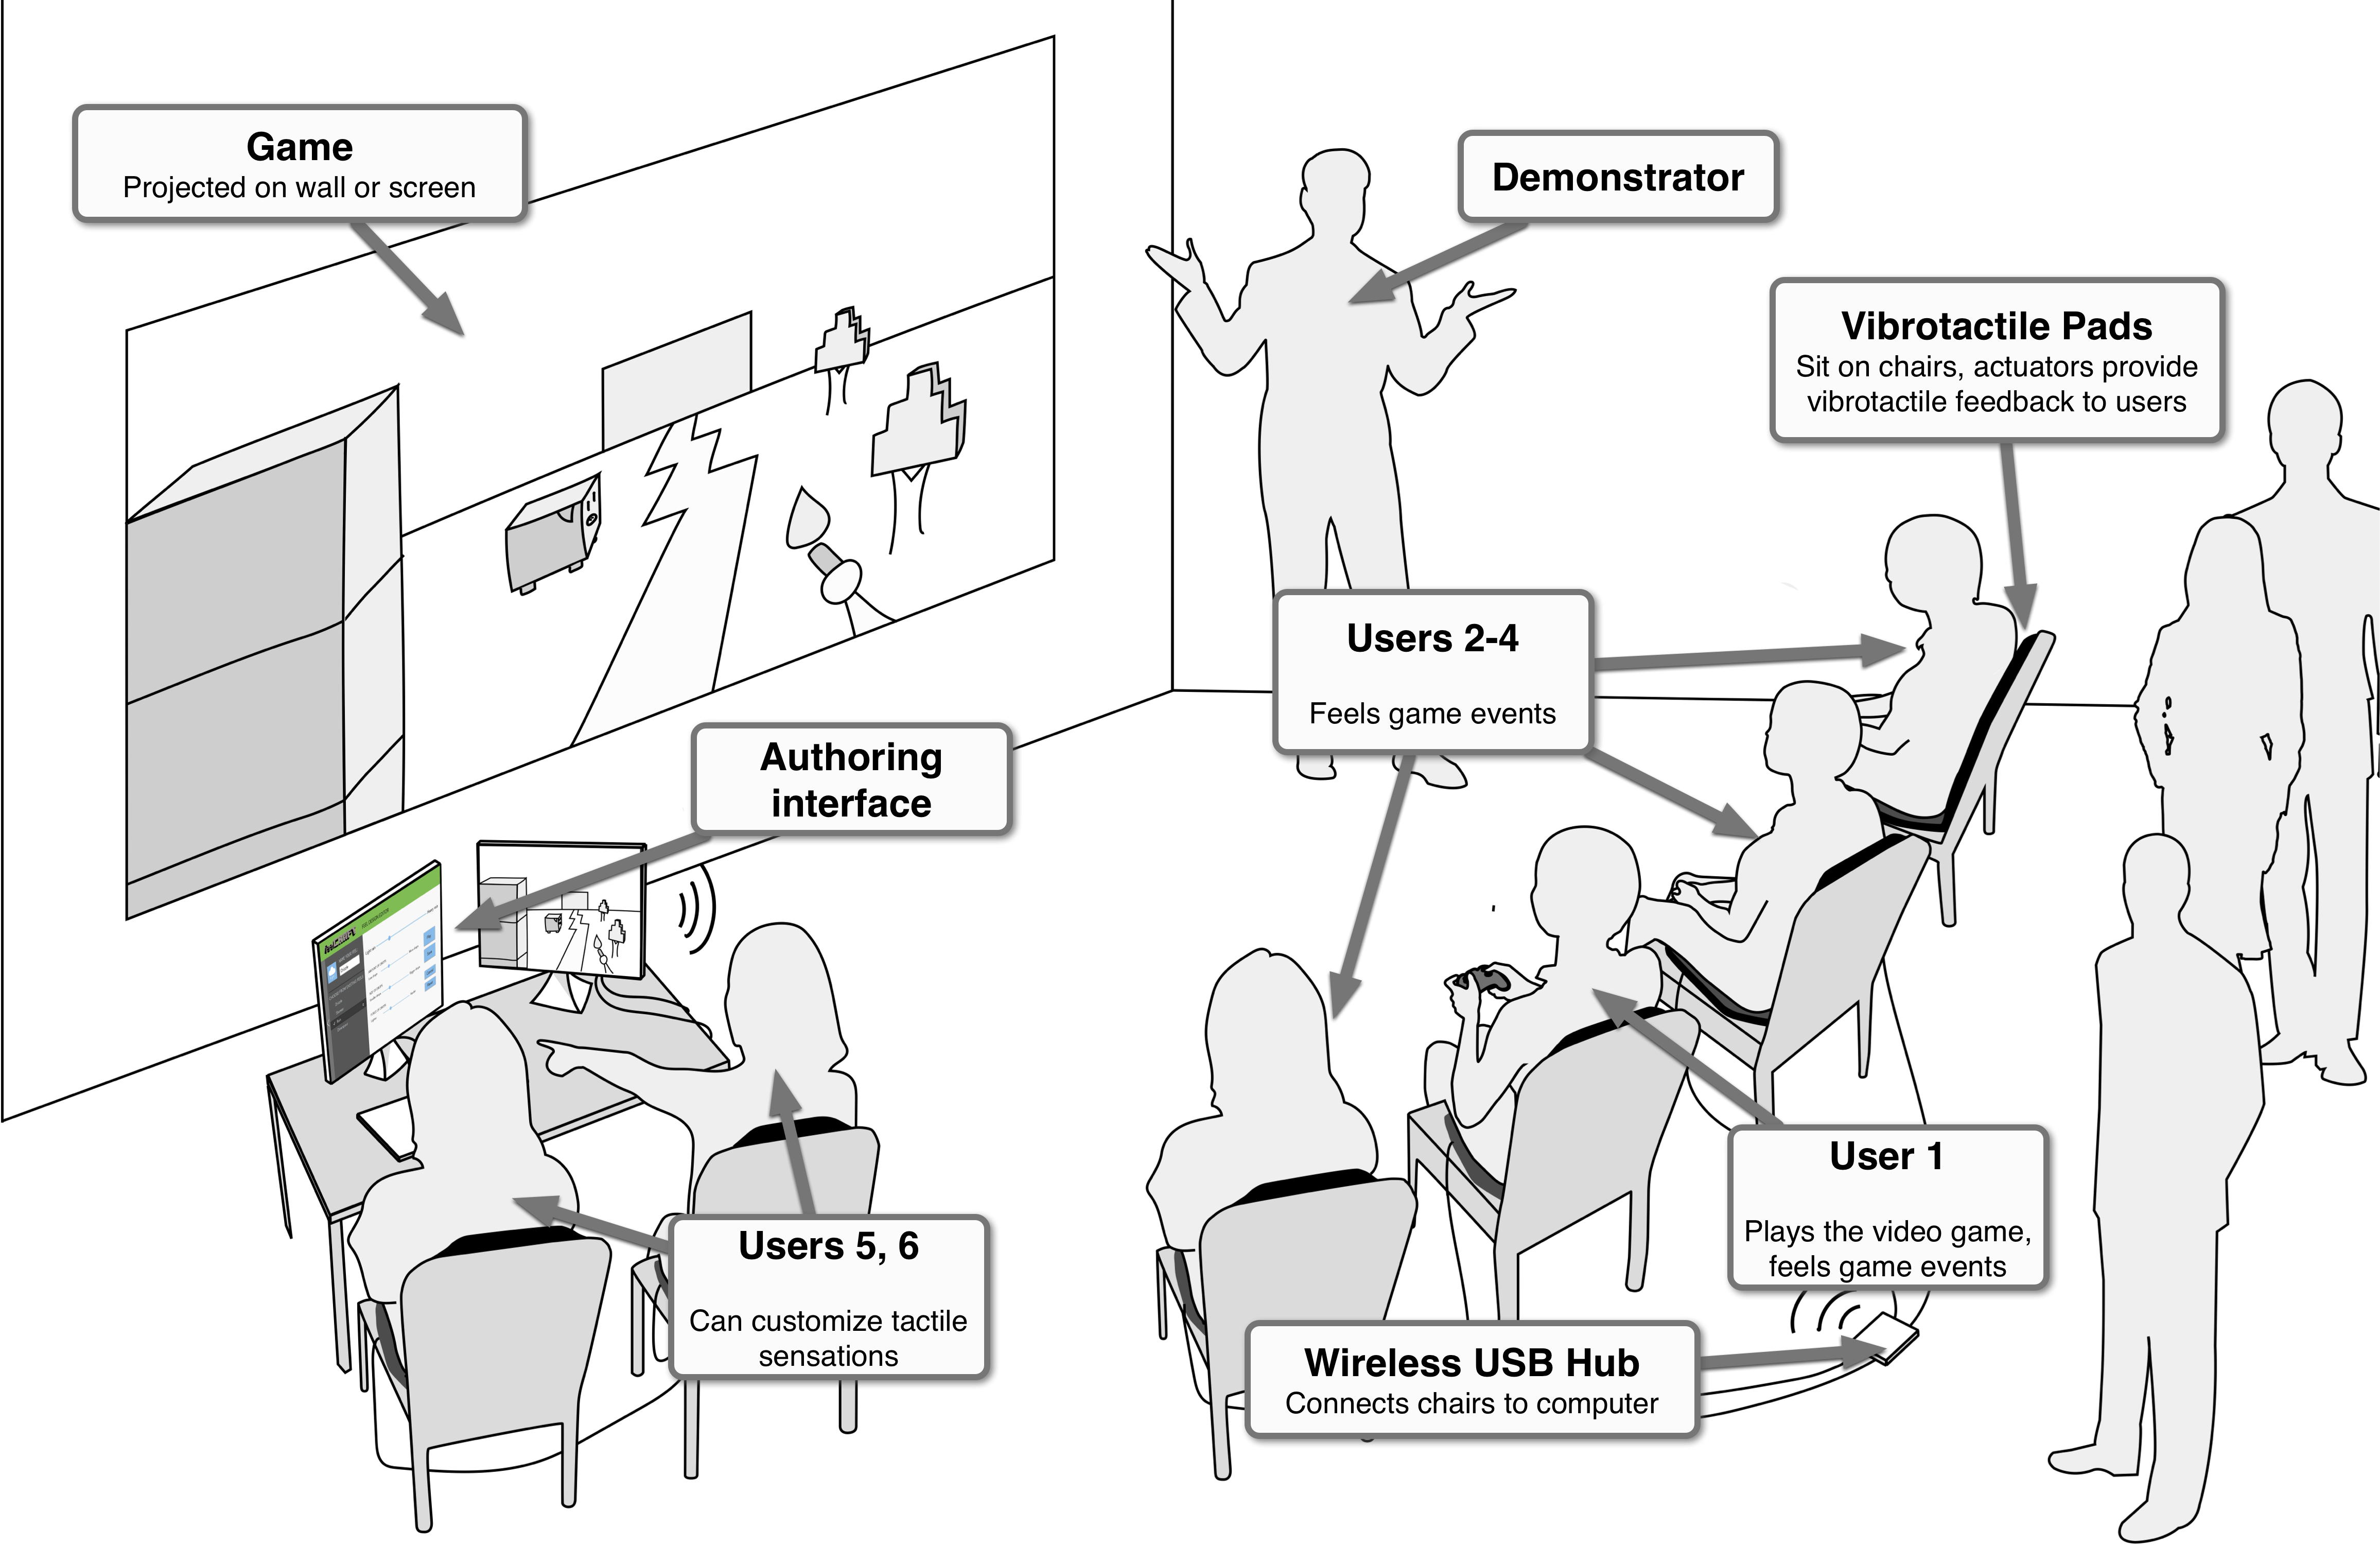
\includegraphics[width=\textwidth]{feelcraft/FeelcraftMockupLabeled} 
   \caption{Mockup for FeelCraft demo system.}
   \label{fig:feelcraft:mockup}
\end{figure}


\subsection{Application Ecosystem}

\begin{figure}[htbp] %  figure placement: here, top, bottom, or page
   \centering
   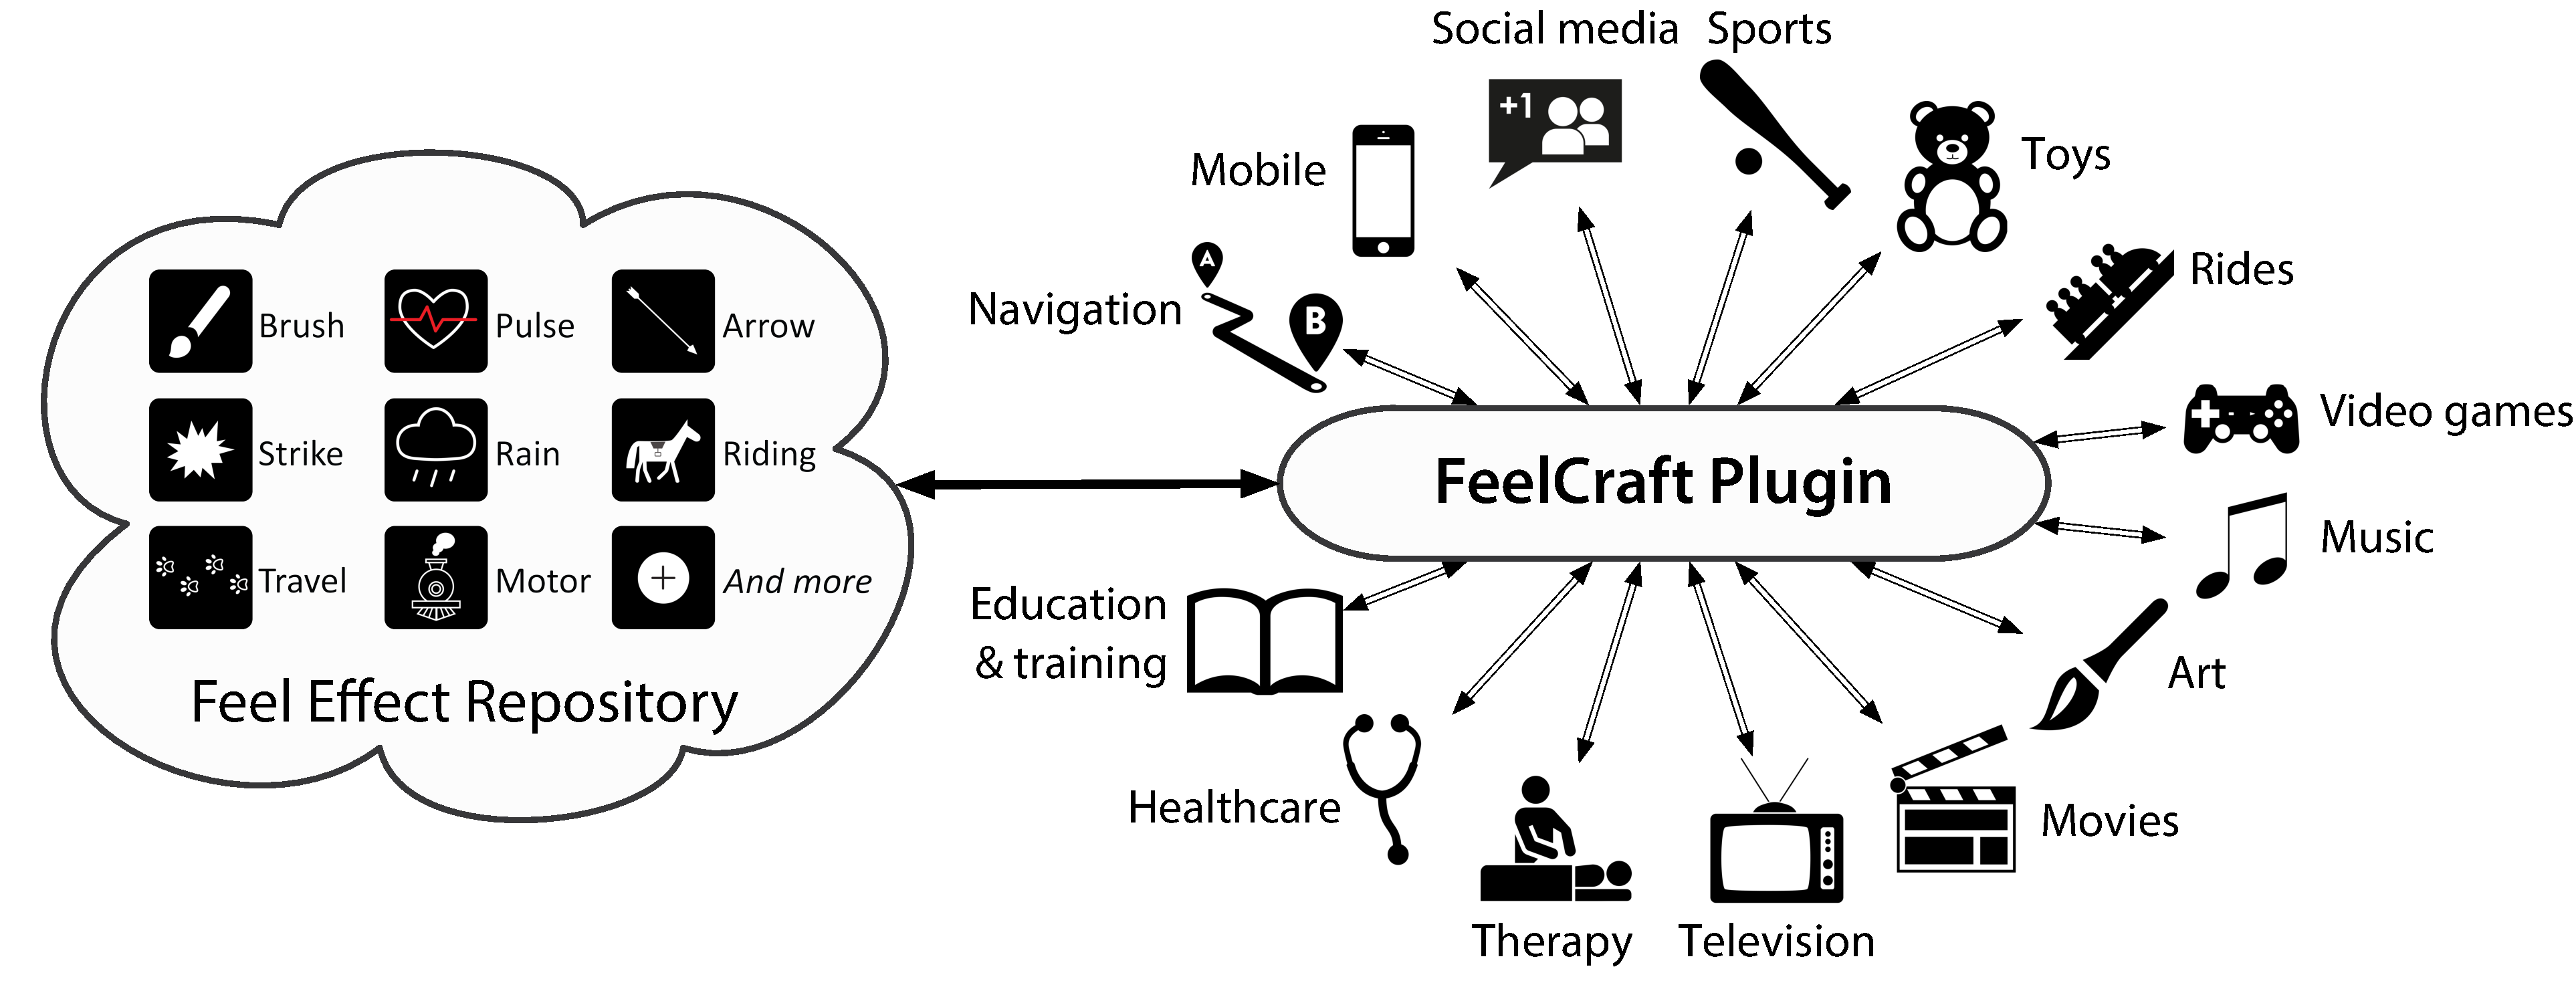
\includegraphics[width=\textwidth]{feelcraft/FeelCraftEcosystem-2014-07-23-1822} 
   \caption{ Application ecosystem for FeelCraft and an FE repository}
   \label{fig:feelcraft:ecosystem}
\end{figure}

FeelCraft plugins are designed to make haptics accessible to end users using existing media and technology. For example, a user may want to assign a custom vibration to a friend's phone number, or add haptics to a game. In this case, a user would download a FeelCraft plugin for their device, browse FEs on an online feel repository, and download FE families they prefer. Once downloaded, the FeelCraft authoring interface allows for customization, as a rain FE for one video game may not quite suit another game. The user could create a new FE for their specific application, and once they were happy with it, upload their custom FE for others to use. If the user wanted to show a friend their FE, they could use the playback system to drive output to multiple devices, or export the FE to a file and send it to them later. Figure 2 illustrates this ecosystem with application areas. Just like the Noun Project for visual icons (http:// thenounproject.com) and downloadable sound effect libraries, we envision online repositories of FEs that can be continually expanded with new FEs by users. Our current FErepository includes six original families described in \cite{Israr2014} and an additional four new families: Ride, Explosion, Fall, and Arrow.




%\subsection{Conclusion}
%In this paper, we have presented FeelCraft, a software plugin that allows users to author, customize, share, and broadcast dynamic tactile experiences with media and user activities. The plugin uses FEs, semantically structured haptic patterns.
%We integrated the FeelCraft plugin with a popular sandbox game, MineCraft. Users can associate six events in the game to corresponding FE, and modify and broadcast to other users to share the haptic experience. The newly authored FEs are saved and shared with other users for communal use via an online FE repository. The pro- posed plugin can also be used with a wide range of entertaining, social, and edu- cational media. Future work includes expanding the FE repository, networked communication and sharing, and supporting output to different haptic device types while maintaining semantic meaning, connecting end users to haptics in an even more accessible manner.

\begin{figure}[htbp] %  figure placement: here, top, bottom, or page
   \centering
   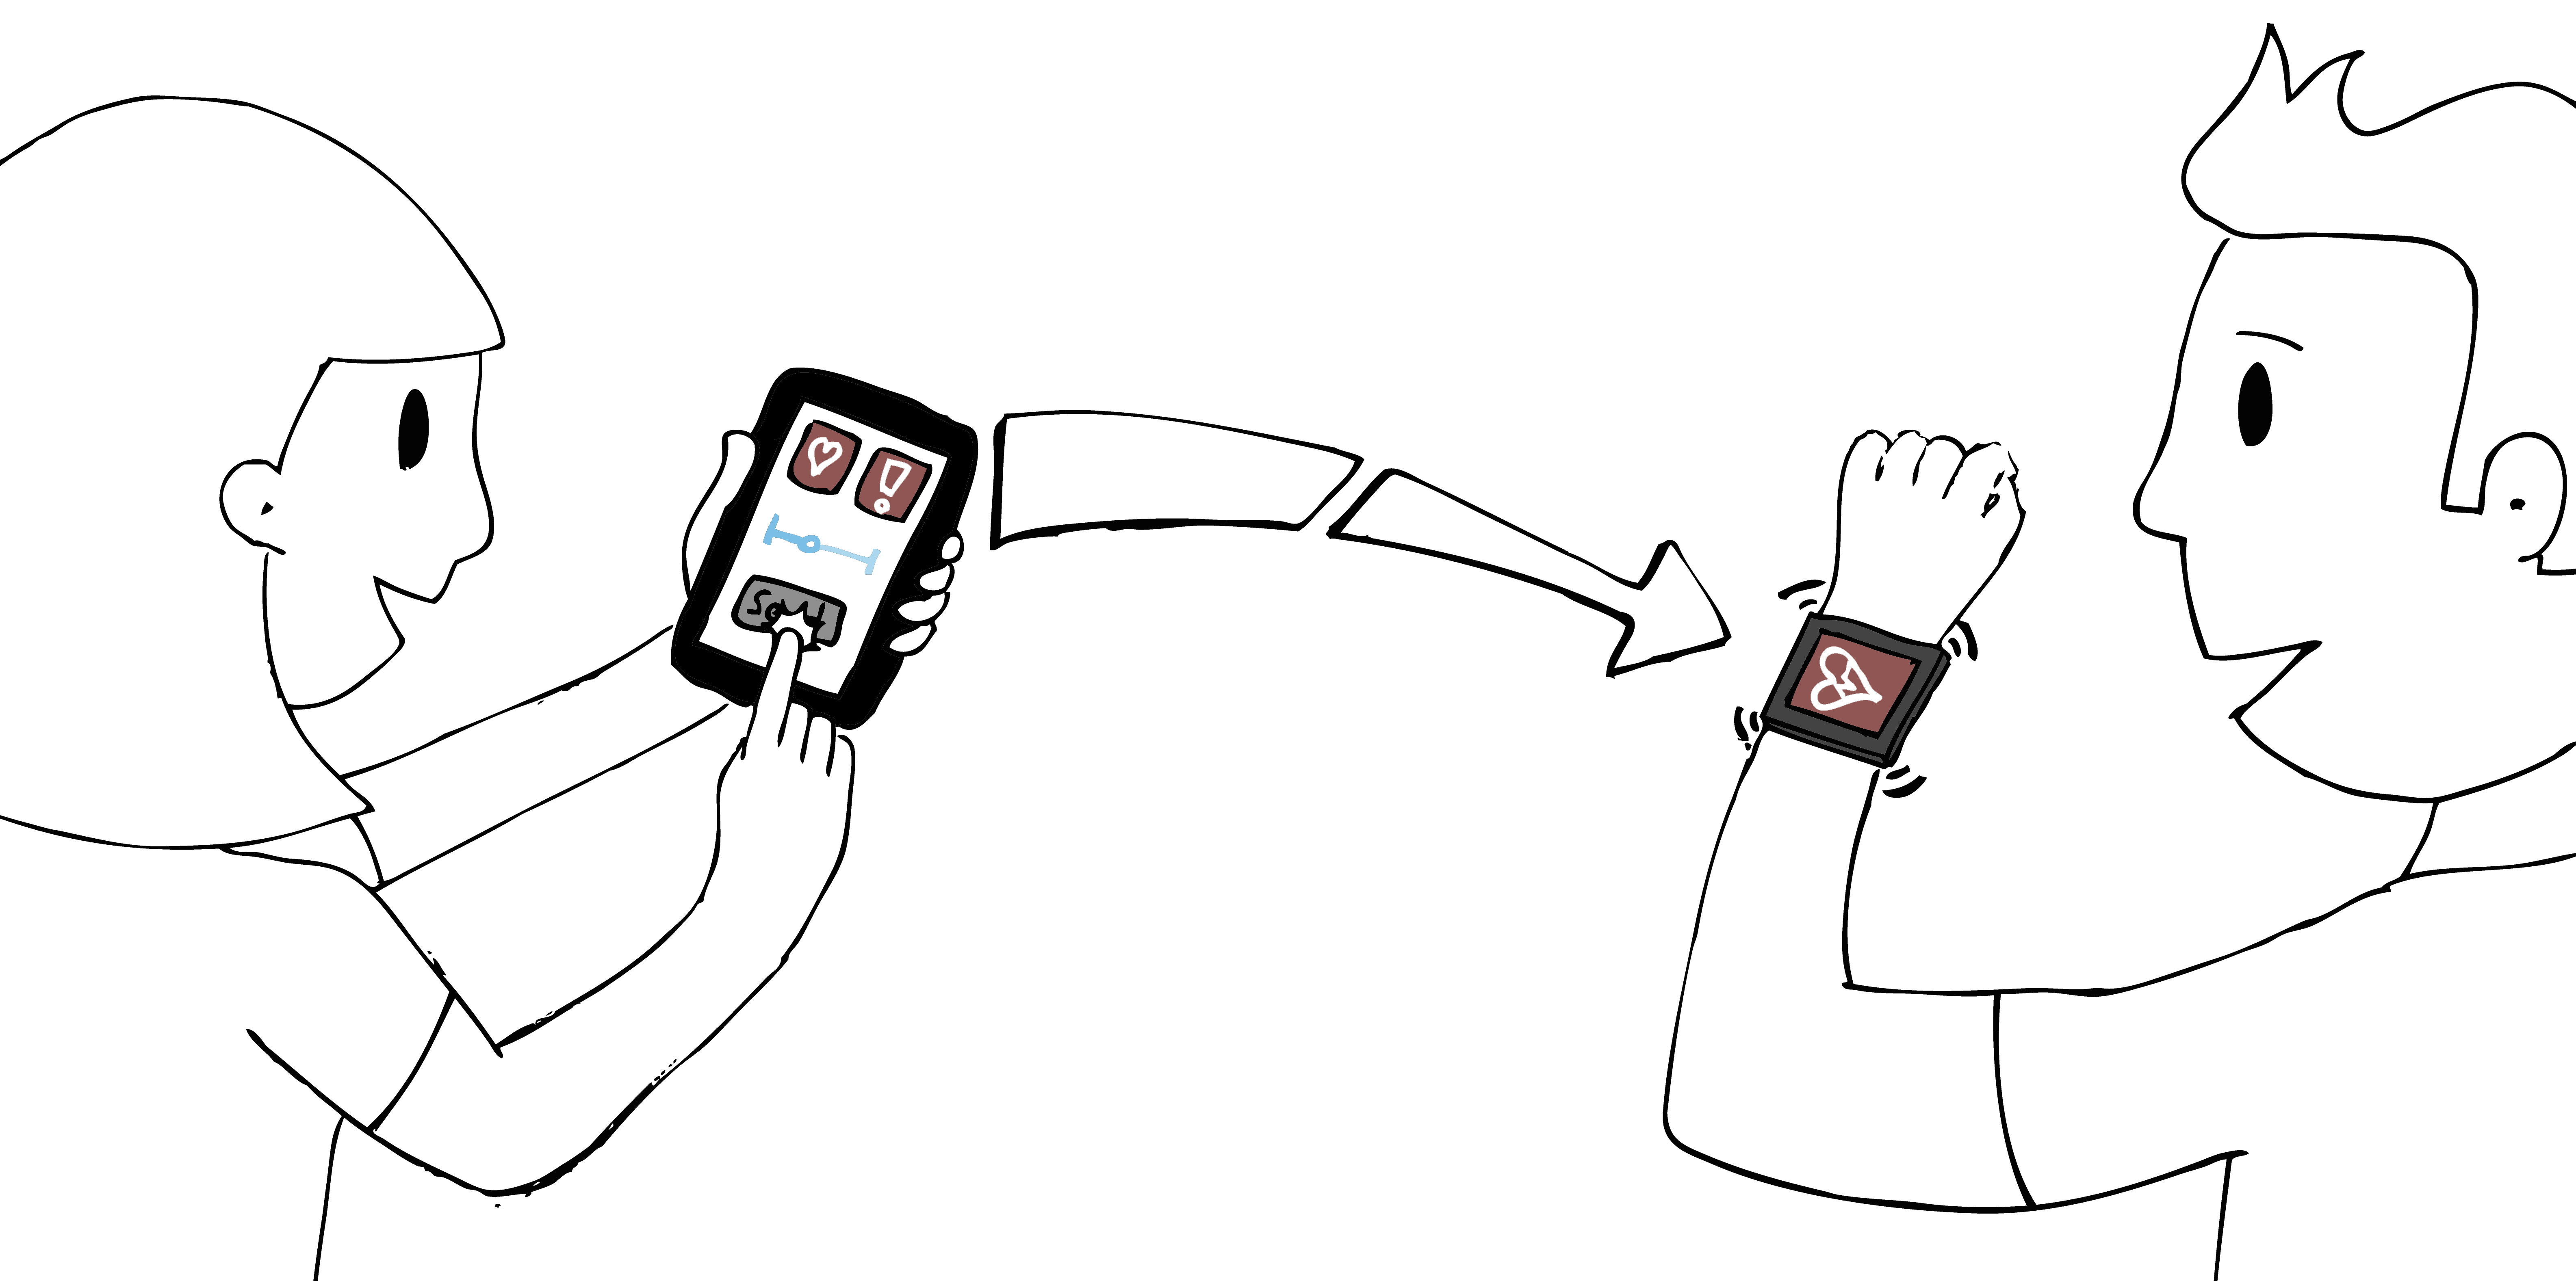
\includegraphics[width=\textwidth]{feelmessenger/Figure1} 
   \caption{Users exchanging expressive haptic messages on consumer embedded devices.}
   \label{fig:feelmessenger:fig1}
\end{figure}



\section{Feel Messenger: Expressive Effects with Commodity Systems}
\label{sec:applications:feelmessenger}
\noindent
In \autoref{sec:applications:feelcraft}, we designed expressive spatial VT Feel Effects using existing infrastructure, using a plugin architecture to link desktop applications to new VT hardware.
In \autoref{sec:applications:feelmessenger}, we look at the expressiveness of existing infrastructure and actuation methods with Android smartphones for customizable VT effects by implementing customizable VT emojis in a chat program, Feel Messenger.
As illustrated previously by \autoref{fig:vib:lofidesign} in \autoref{ch:hapturk}, APIs for vibrotactile feedback are currently limited to a series of pulses.
With Feel Messenger, we were able to produce expressive VT icons for emojis using the built-in Android API, including customizable effects like a heartbeat that varies in both rate and intensity.
We found VT icons were effective when they had an engaging visual icon to frame the vibration, \eg, a cat emoji helped the user understand purring vibration was a purr.
\autoref{fig:feelmessenger:fig1} presents a concept sketch.

%Touch is particularly significant in interpersonal communication [3].
%Ranging from mutual user interactions, such as handshakes and hugs, to directing a user's attention by poking or tapping on the shoulder; the channel of touch has also been used in children games in which one child draws patterns on another child's body usin ga finger, and the recipient child guesses what is drawn on the body [7].
%Many authors have explored the haptic channel to artificially communicate, enhance and augment interactions on custom-made handheld and wearable devices [3, 4, 5, 16]. This paper explores the use of haptic feedback in social interactions, such as instant messaging, social networking and everyday social use on embedded mobile devices.
%
%Current consumer devices, such as mobile devices, watches and hand controllers, are equipped with a single vibrotactile (VT) motor that usually alerts users for incoming calls or messages, and/or for text entry and ?clicks? [8]. These actuators are popular due to low cost and power requirements, small size and weight, convenient packaging and simple control electronics. The challenge is to create meaningful, expressive and interactive haptic feedback in-between users using only a single low-bandwidth VT motor and with limited computational resources in embedded devices.
%
%Recently, Israr and colleagues [9] have demonstrated that a class of haptic patterns, called feel effects (FEs), could be defined in a parametric structure, called a family. By tuning parameters of these families, users control the semantic interpretation of haptic patterns using the same logic as they would use in normal language. This interpretation of haptic patterns not only allows users to communicate more expressive haptic content, but also to personalize the right haptic pattern for social and interpersonal communication. Such feel effects have also shown to improve early reading comprehension scores in [18].
%
%In this paper, we implement Feel Messenger, a social and instant messaging (IM) application that allows users to share, express and communicate haptic patterns in a structured and economical way on current consumer devices (i.e., using the embedded VT motor). We introduce ?feelbits? and ?feelgits?, haptic structures that allow succinct and eloquent network communication and reduce bandwidth and latency between devices. By allowing users to share and personalize haptic content, we hope to extend the capabilities of handheld and wearable devices for more interactive use among consumers.
%
%This paper is organized as follows: After a brief background, we present the Feel Messenger application. Next, we explore the vocabulary of haptic patterns and present a pilot study to evaluate the usability of the application.
%
%\subsection{Background}
%The idea of haptic feedback for instant messaging and social networking has been demonstrated in the past, however, previous work lacked expressive and meaningful haptic interactions connected to a semantic language. In these studies, user gestures, pre- programmed tactile patterns and ?feels? were transmitted using custom devices and through multiple actuators [2, 11-14, 17].
%
%Force feedback devices are not applicable for mobile applications, as they need to be coupled with the ground. Shape-changing features and vibratory grids have been explored to convey emotions, textures and directional cues on handheld devices [6, 8]. A few commercial libraries and APIs are also available to add haptics experiences in current mobile devices [1].
%
%These libraries allow programmers to select from a predefined list of haptic patterns and embed them in their application. All patterns are stored in the device?s memory and users have limited flexibility in personalizing haptic patterns for rich and expressive communication. Recently, Seifi and colleagues [15] have shown that participants preferred customization of VT patterns in social settings, and did not prefer predefined patterns.
%
%Therefore, we present a compact and expressive haptic authoring and sharing protocol and implement it on a typical mobile device. The protocol can be extended for other social networking apps, such as twitter, emails, etc., running on tablets, watches, controllers and other embedded devices.
%

\subsection{Feel Messenger Application}
In this section, we present the architecture (backend) and user interface (frontend) of a messenger application that allows users to create and share haptic content through a network connection. The critical components of the application are shown in Figure 2.

\inlineHeading{Architecture}
To account for the limited computation, storage and communication capabilities of a simple microcontroller unit, we introduce feelbits and feelgits. Feelgits (short from ``feel widgets") are installed piece of software that define parametric compositions of a set of haptic patterns (called a family). Feelbits are parametric settings of a feelgit to produce a particular haptic pattern (called a feel effect \cite{Israr2014}). For example, the feelgit of pulse is defined as two successive onsets of vibration, separated by a timing parameter. The feelbits are timing and intensity of onset parameters. Therefore, by varying feelbits, a user can personalize the haptic effect to be calm (low intensity, long temporal separation) or racing (high intensity, short temporal separation) heartbeat.

A library of haptic patterns is stored as parametric models (feelgits) with preset parameters (feelbits). New feelgits and feelbits can be downloaded, personalized and saved. The haptic engine idly waits for incoming haptic messages and renders haptic patterns on demand. Once the message is received, the corresponding feelgit is executed with parameters defined as feelbits. Once the pattern is completely rendered, the engine waits idly for the next message.

Additionally, the response characteristics of the VT motor are also stored in the memory. These characteristics are generally represented by simple first-order functions relating the digital value (such as data byte) to the perceived intensity judged by users \cite{Jones2008tactors}, which could be used to maintain the quality of experience across wide variety of mobile phones and hardware technologies.

Finally, we introduce a communication protocol that shares feelgits and feelbits along with text messages. For example, the frontend application sends a function playpattern(``pulse", p1, p2) to play the feelgit pulse with parameters defined as feelbits p1 and p2; or playpulse(``soft") plays a predefine soft pulse. Note that in order for the device to play a haptic pattern, the corresponding feelgit must be stored in the device; the communication packet includes feelbits and the name or id of the corresponding feelgit.


%\begin{figure}[htbp] %  figure placement: here, top, bottom, or page
%   \centering
%   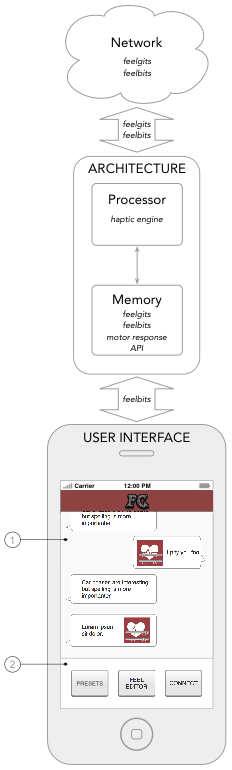
\includegraphics[width=0.5\textwidth]{feelmessenger/fig2} 
%   \caption{The backend software architecture and the frontend user interface of the Feel Messenger app.}
%   \label{fig:feelmessenger:fig2}
%\end{figure}


%
%\inlineHeading{User Interface}
%The frontend of the application is shown in Figure 2. In addition to conventional text and image entries, the Feel Messenger interface allows users to play, personalize and share haptic patterns. The components of the interface are explained below.

%\inlineHeading{Messenger Interface}
%The message interface, Figure 2 (1), is kept almost the same as a typical IM interface on current devices. However, this can be easily adapted to emails, Twitter feeds or other social media timelines. Aligned to the left are received messages and those aligned to the right are the sent or entered messages. Along with the message is an icon indicating that a haptic effect has been attached to the message. Once the message is received, the application triggers the haptic engine to play the haptic pattern. The user can replay the message by clicking on the message or the accompanying icon. Multiple patterns can also be embedded in a single message. Simultaneous effects are sent by using ?|? (vertical bar) between two icons, otherwise the effects are played in the same order as the icons in the message.
%
%Below the message interface are three icons buttons, shown in Figure 2 (2). The leftmost icon allows users to attach a predefined FE (Figure 3A). The center icon opens a Feel Editor display (Figure 3B), and the right most buttons connects to the users (Figure 3C).

\inlineHeading{Predefined Patterns}
The predefined patterns allow users to quickly attach a haptic pattern to the IM. These patterns can be stored from incoming messages or created by using stored haptic families. Each pattern is defined by a set of feelbits that plays when the corresponding feelgit is executed. These presets can be shown as text, images or emotion icons.

\inlineHeading{Authoring interface}
The Feel Editor displays available FE families (feelgits) and allows users to personalize, play, save and share haptic patterns.
%(Figure 3B).
By clicking a FE icon, sliders corresponding to parameters (feelbits) are enabled. These sliders may have labels corresponding to physical parameters, such as amplitude or duration of vibration; however, we have used semantic labeling that may correspond to single or multiple parameters. Once the sliders are adjusted, the user can play, save or attach the haptic pattern to the IM.


%\begin{figure}[htbp] %  figure placement: here, top, bottom, or page
%   \centering
%   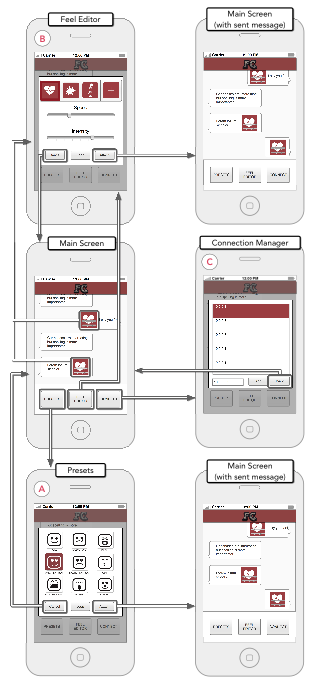
\includegraphics[width=\textwidth]{feelmessenger/fig3} 
%   \caption{Program flow diagram of the Feel Messenger application.}
%   \label{fig:feelmessenger:fig3}
%\end{figure}
%


\subsection{Haptic Vocabulary}
The vocabulary of haptic effect is critical for expressive and precise communication between users. In this preliminary implementation, we explore three types of haptic vocabularies. Type 1 is adapted from feel effects defined in \cite{Israr2014}, where haptic patterns are semantically characterize by a phrase. Type 2 is change in physical parameters as in \cite{Brewster2004,MacLean2003} but can also be simultaneously played with feel effects. Type 3 predefined coded patterns.
\autoref{fig:feelmessenger:fig4} shows the icons for haptic language. Note, that the two feel effects cannot be simultaneously played. This will result in overflow of the user's bandwidth, especially with a low-fidelity VT actuator.


\begin{figure}[htbp] %  figure placement: here, top, bottom, or page
   \centering
   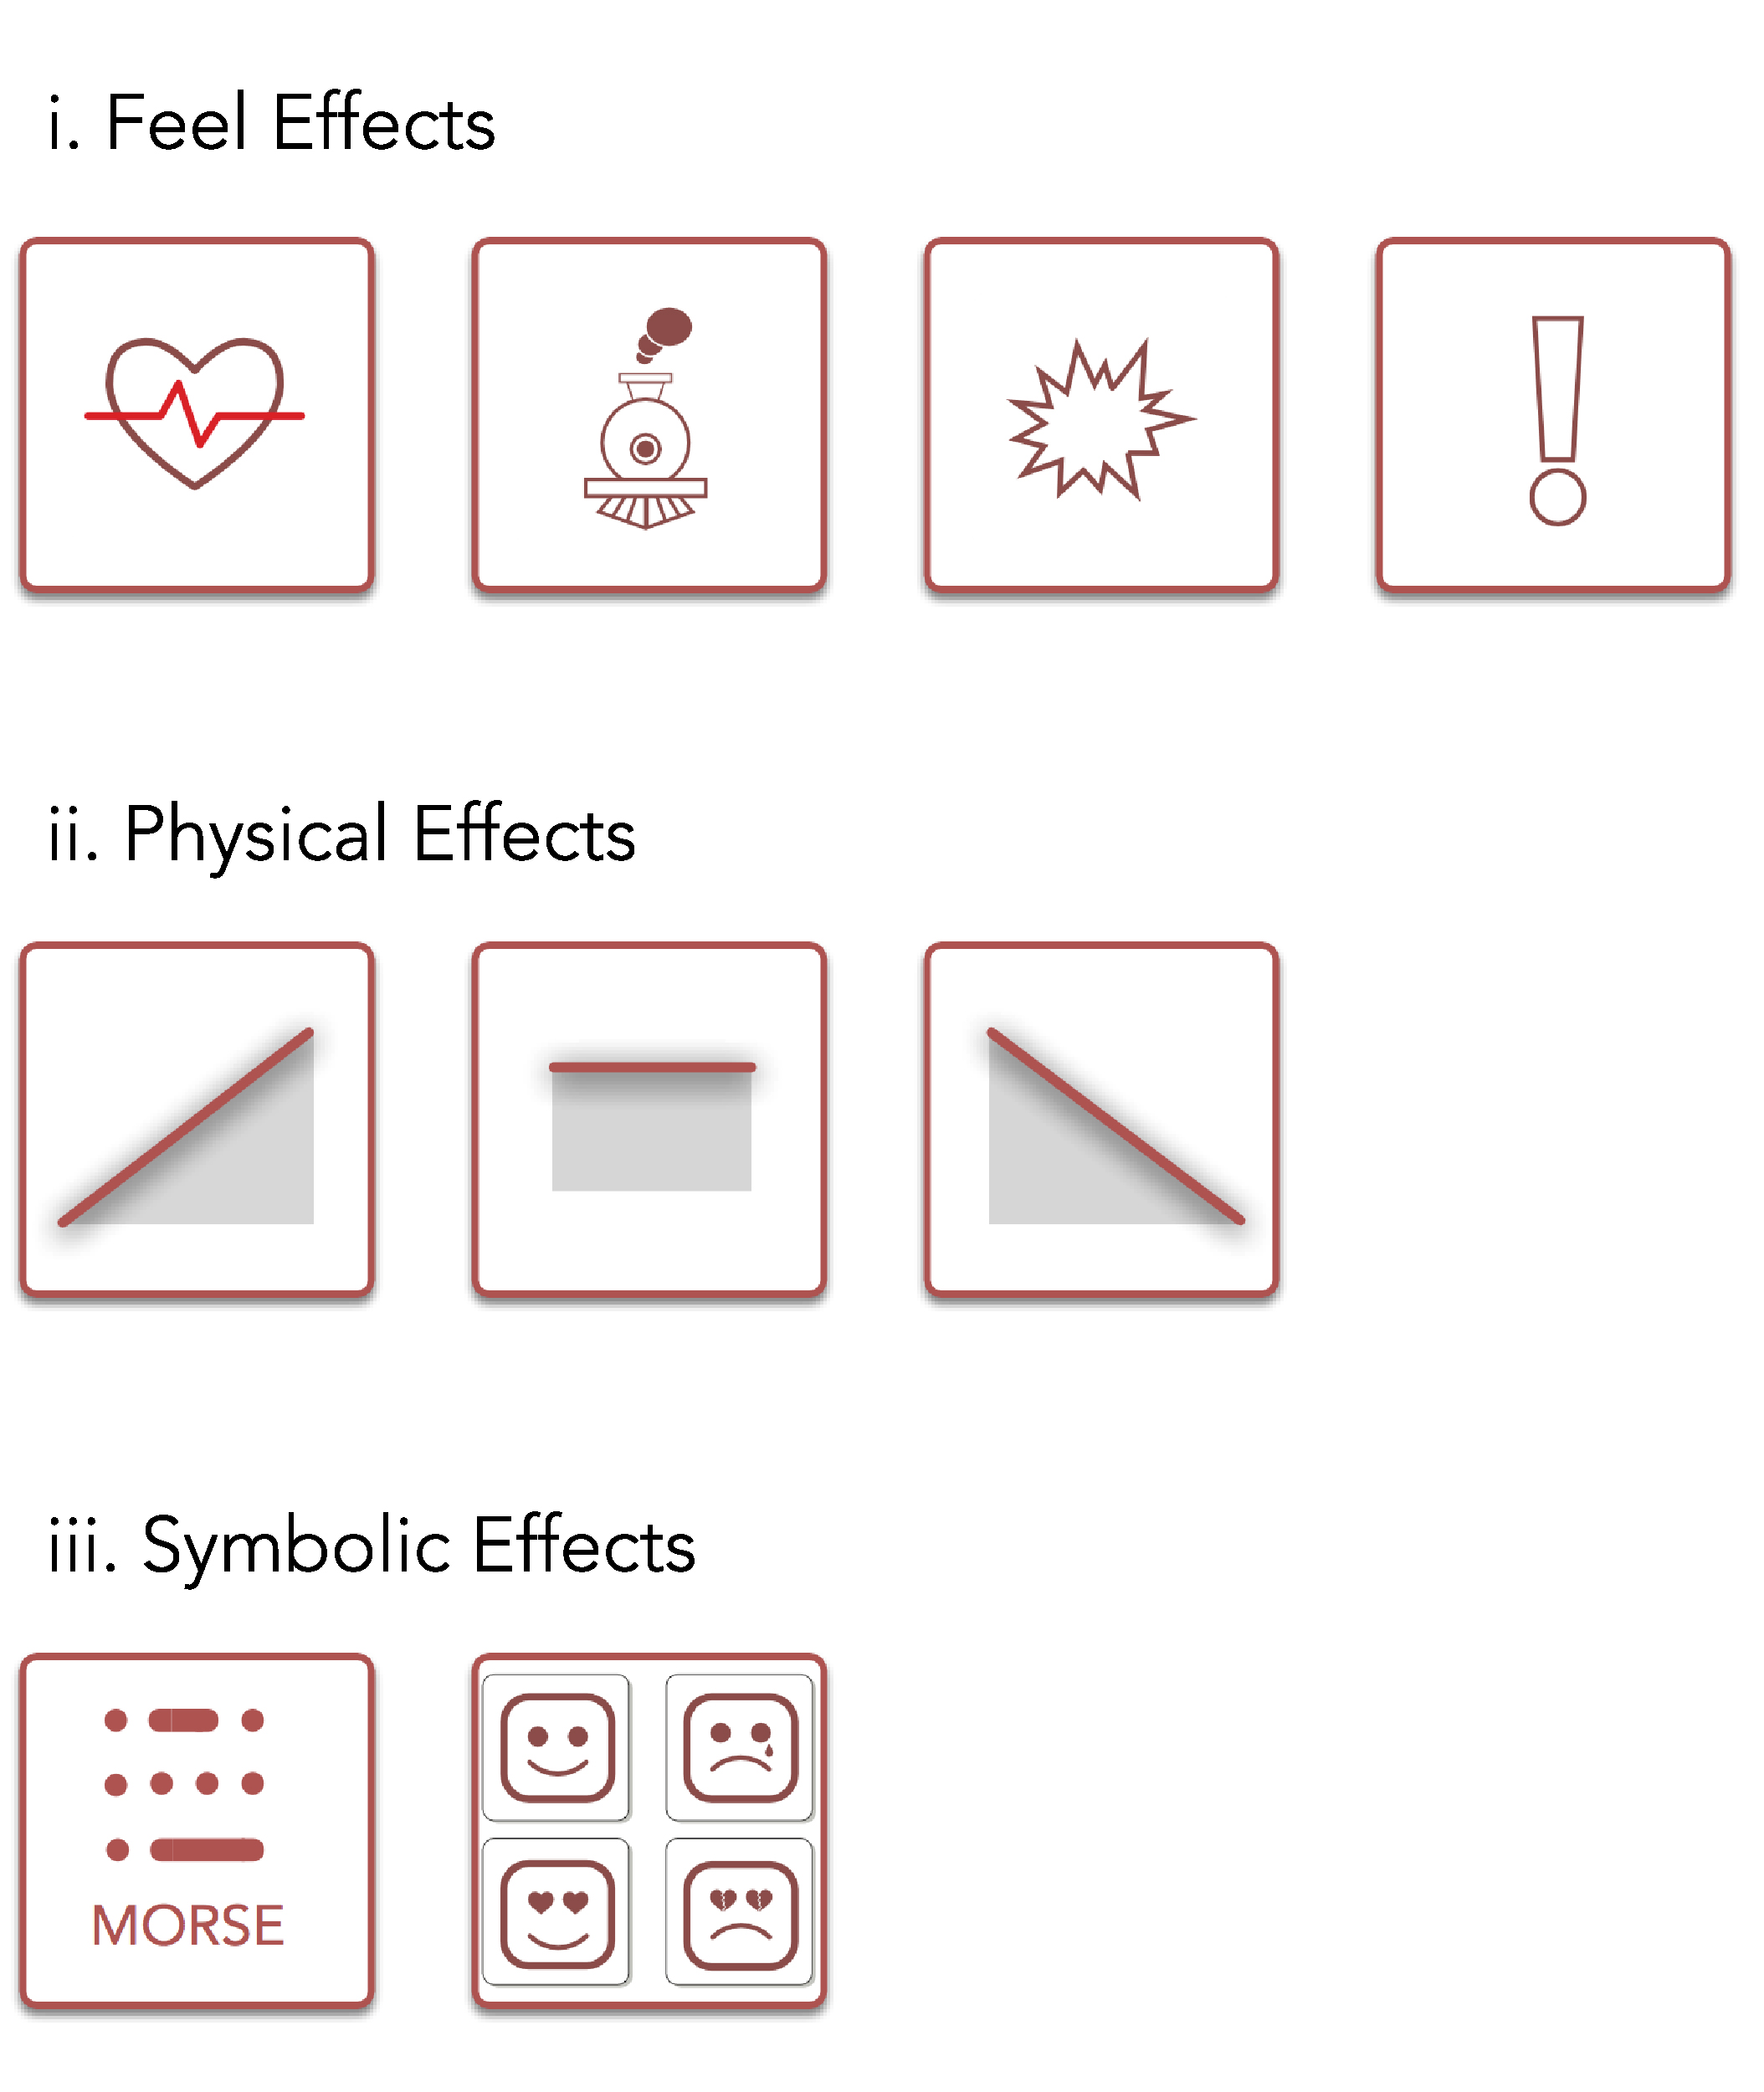
\includegraphics[width=0.6\textwidth]{feelmessenger/fig4} 
   \caption{Graphical representation of haptic vocabularies and icons.}
   \label{fig:feelmessenger:fig4}
\end{figure}


\begin{figure}[htbp] %  figure placement: here, top, bottom, or page
   \centering
   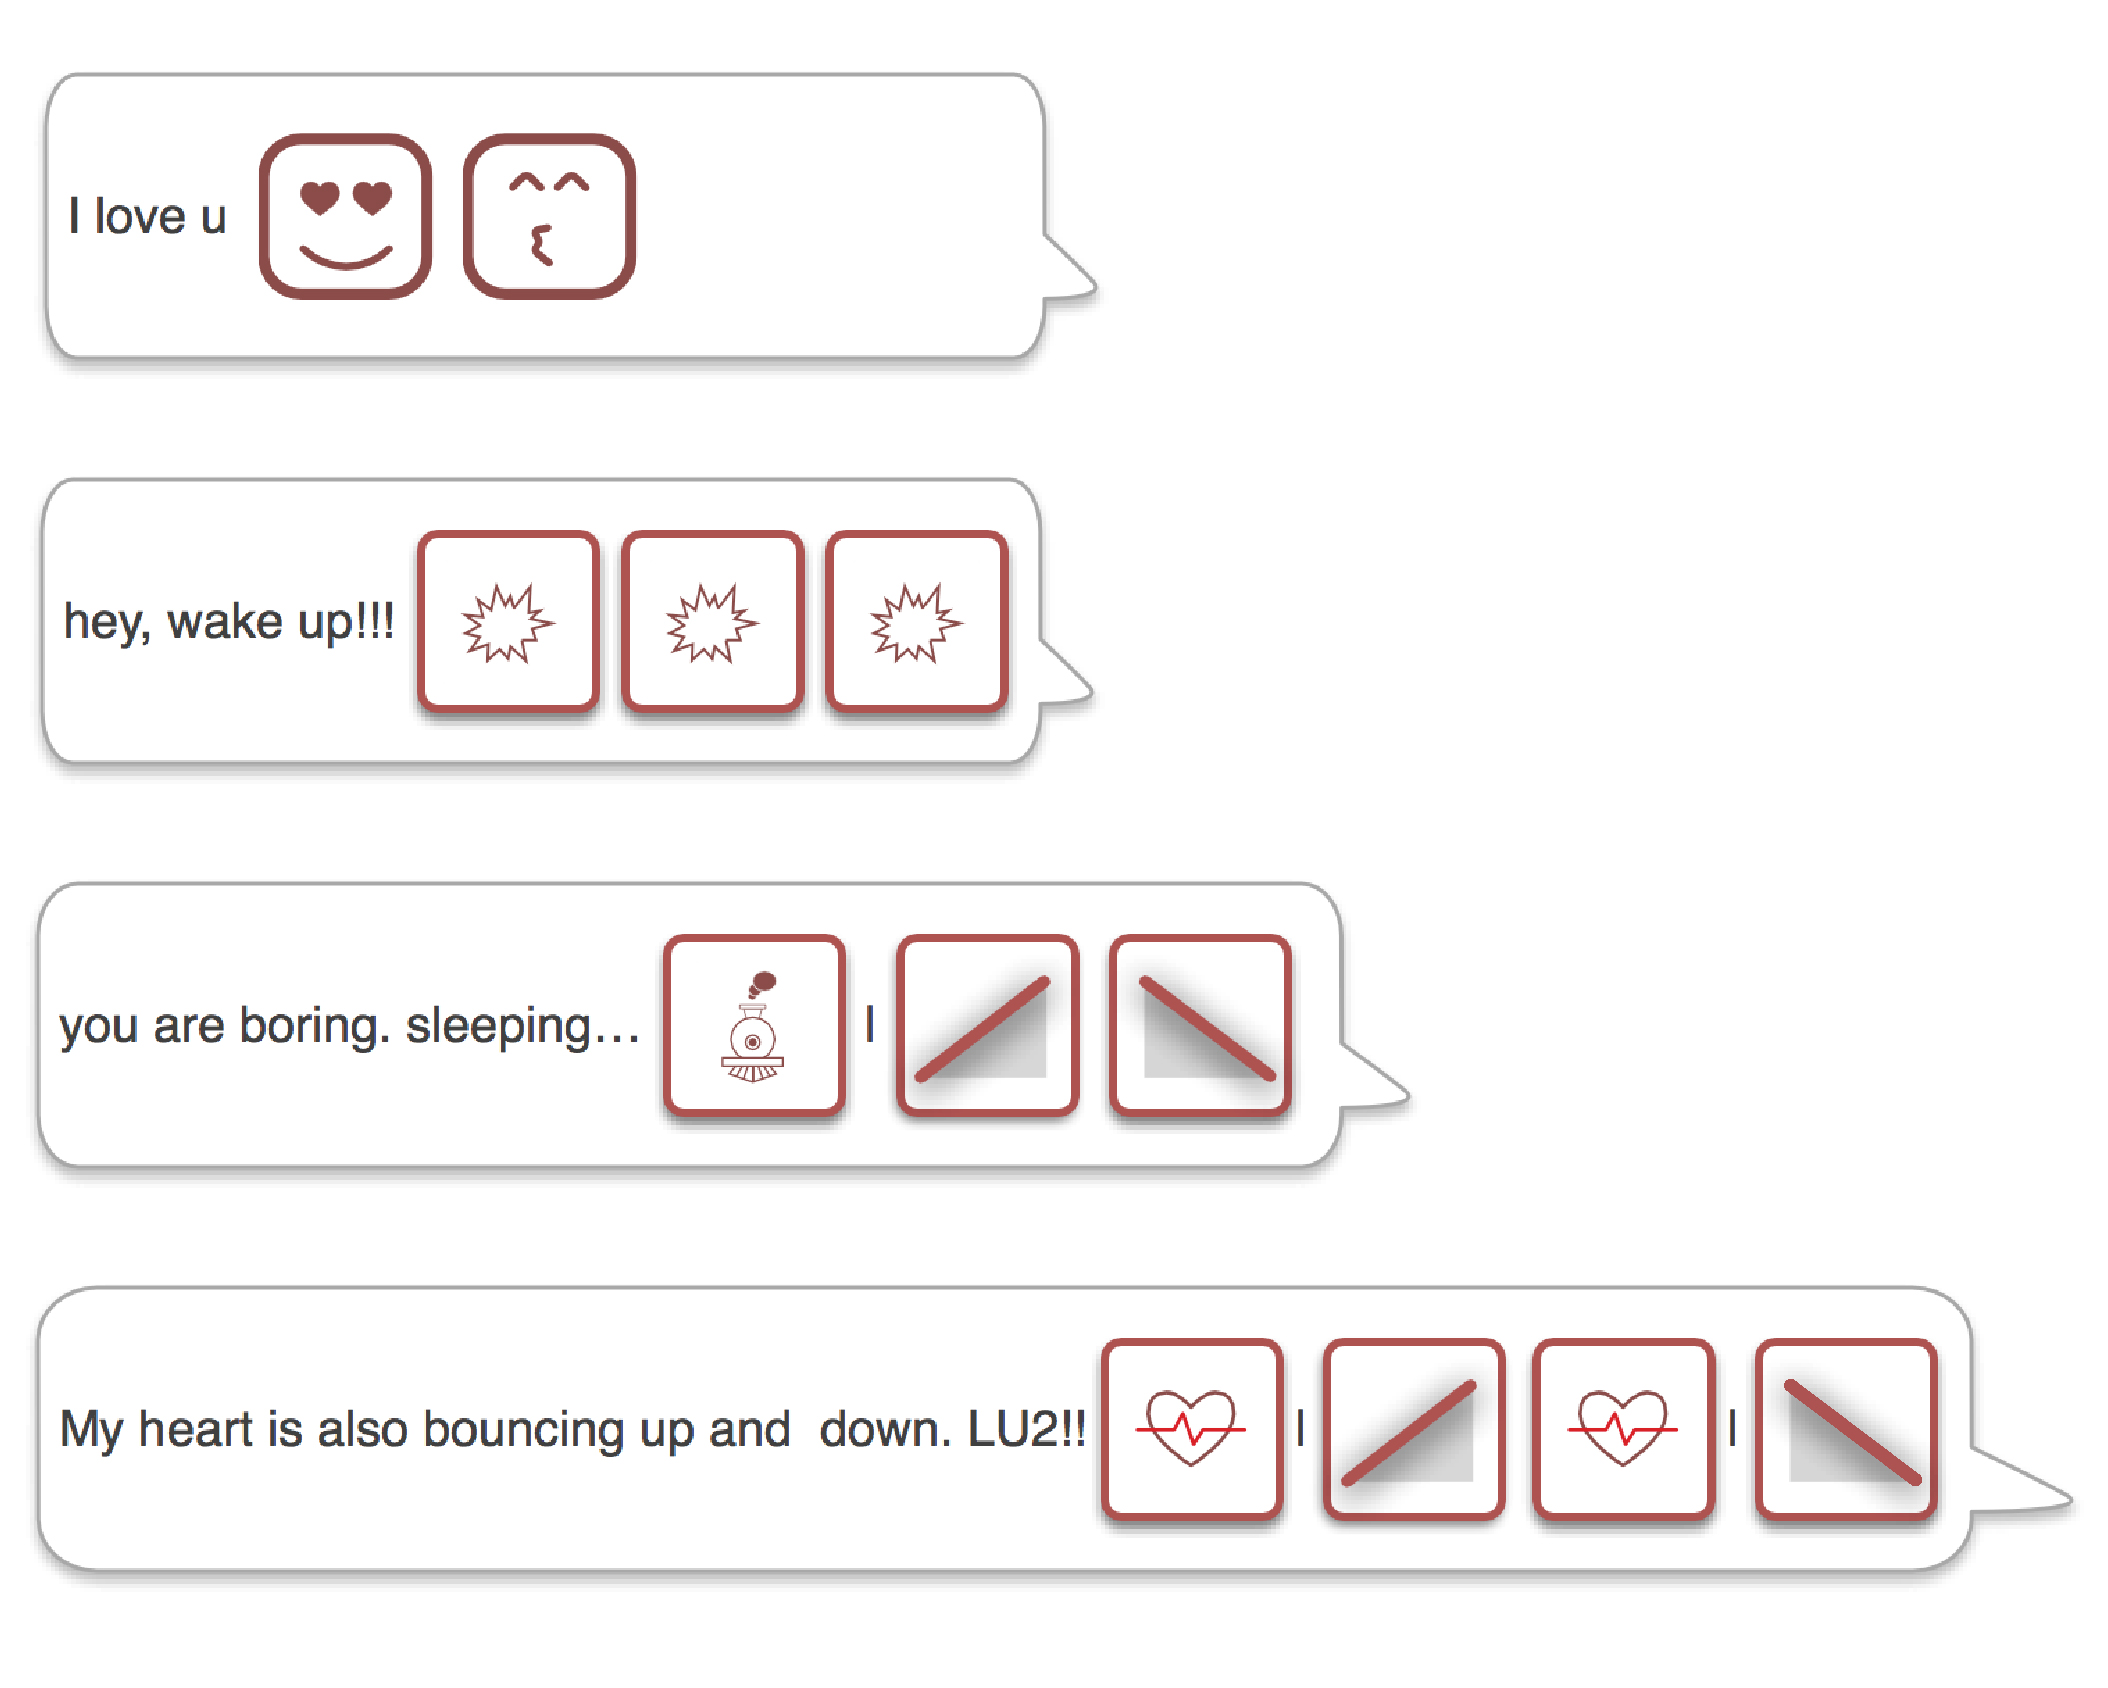
\includegraphics[width=0.6\textwidth]{feelmessenger/fig5} 
   \caption{Some examples of expressive haptic messages embedded with normal text messages.}
   \label{fig:feelmessenger:fig5}
\end{figure}


\inlineHeading{Type 1: Feel Effects}
A set of feel effects is defined that delivers emotional, attentional and contextual effects. They are:
\begin{description}
	\item[Pulse:] Two successive onsets of vibration; speed (slow/fast) and intensity (weak/strong). Used as pulsation and heartbeat (calm/racing).
	\item[Motor:] A 4-second modulated vibration; intensity (soft/loud) and speed (slow/fast) are parameters. Used as snoring, breathing, purring, engine rumble, etc.
	\item[Strike:] A single onset of vibration; duration (short/long) and intensity of vibration are parameters. Used for tap, poke, jab and punch.
	\item[Urgency:] a burst of vibrations; intensity (weak/strong) and temporal separation between pulses (low/high urgency) are parameters. Used for alerting users and expressing urgency.
\end{description}

\inlineHeading{Type 2: Physical Effects}
These effects are associated with direct variation in tactile patterns. Previous studies (\eg, \cite{Brewster2004,MacLean2003}) have used variation in amplitude, duration as typical variation. Our library includes:

\begin{description}
	\item[Ramp-up:] gradual increase in intensity; parameters are peak intensity and the rate of increase.
	\item[Ramp-down:] gradual decrease in intensity; parameters are peak intensity and the rate of decrease.
	\item[Spacer:] keeps steady intensity; parameters are intensity and duration. This can be used for putting a delay (or spaces) between two haptic effects.
\end{description}

These effects create new haptic effects and can also be combined with feel effects. Such as the message Ramp-up | Motor followed by Ramp-down creates a new pattern that gradually increases the rumbling and then decays linearly as shown in \autoref{fig:feelmessenger:fig5}.

\inlineHeading{Type 3: Coded Effects}
This type demonstrates symbolic vocabularies, such as one adapted from International Morse Code that consists of pre-stored pulses of dots and dashes. Other examples can be vibratese language \cite{Tan1997}, emoticon, and input from peripheral sensors.



\begin{figure}[htbp] %  figure placement: here, top, bottom, or page
   \centering
   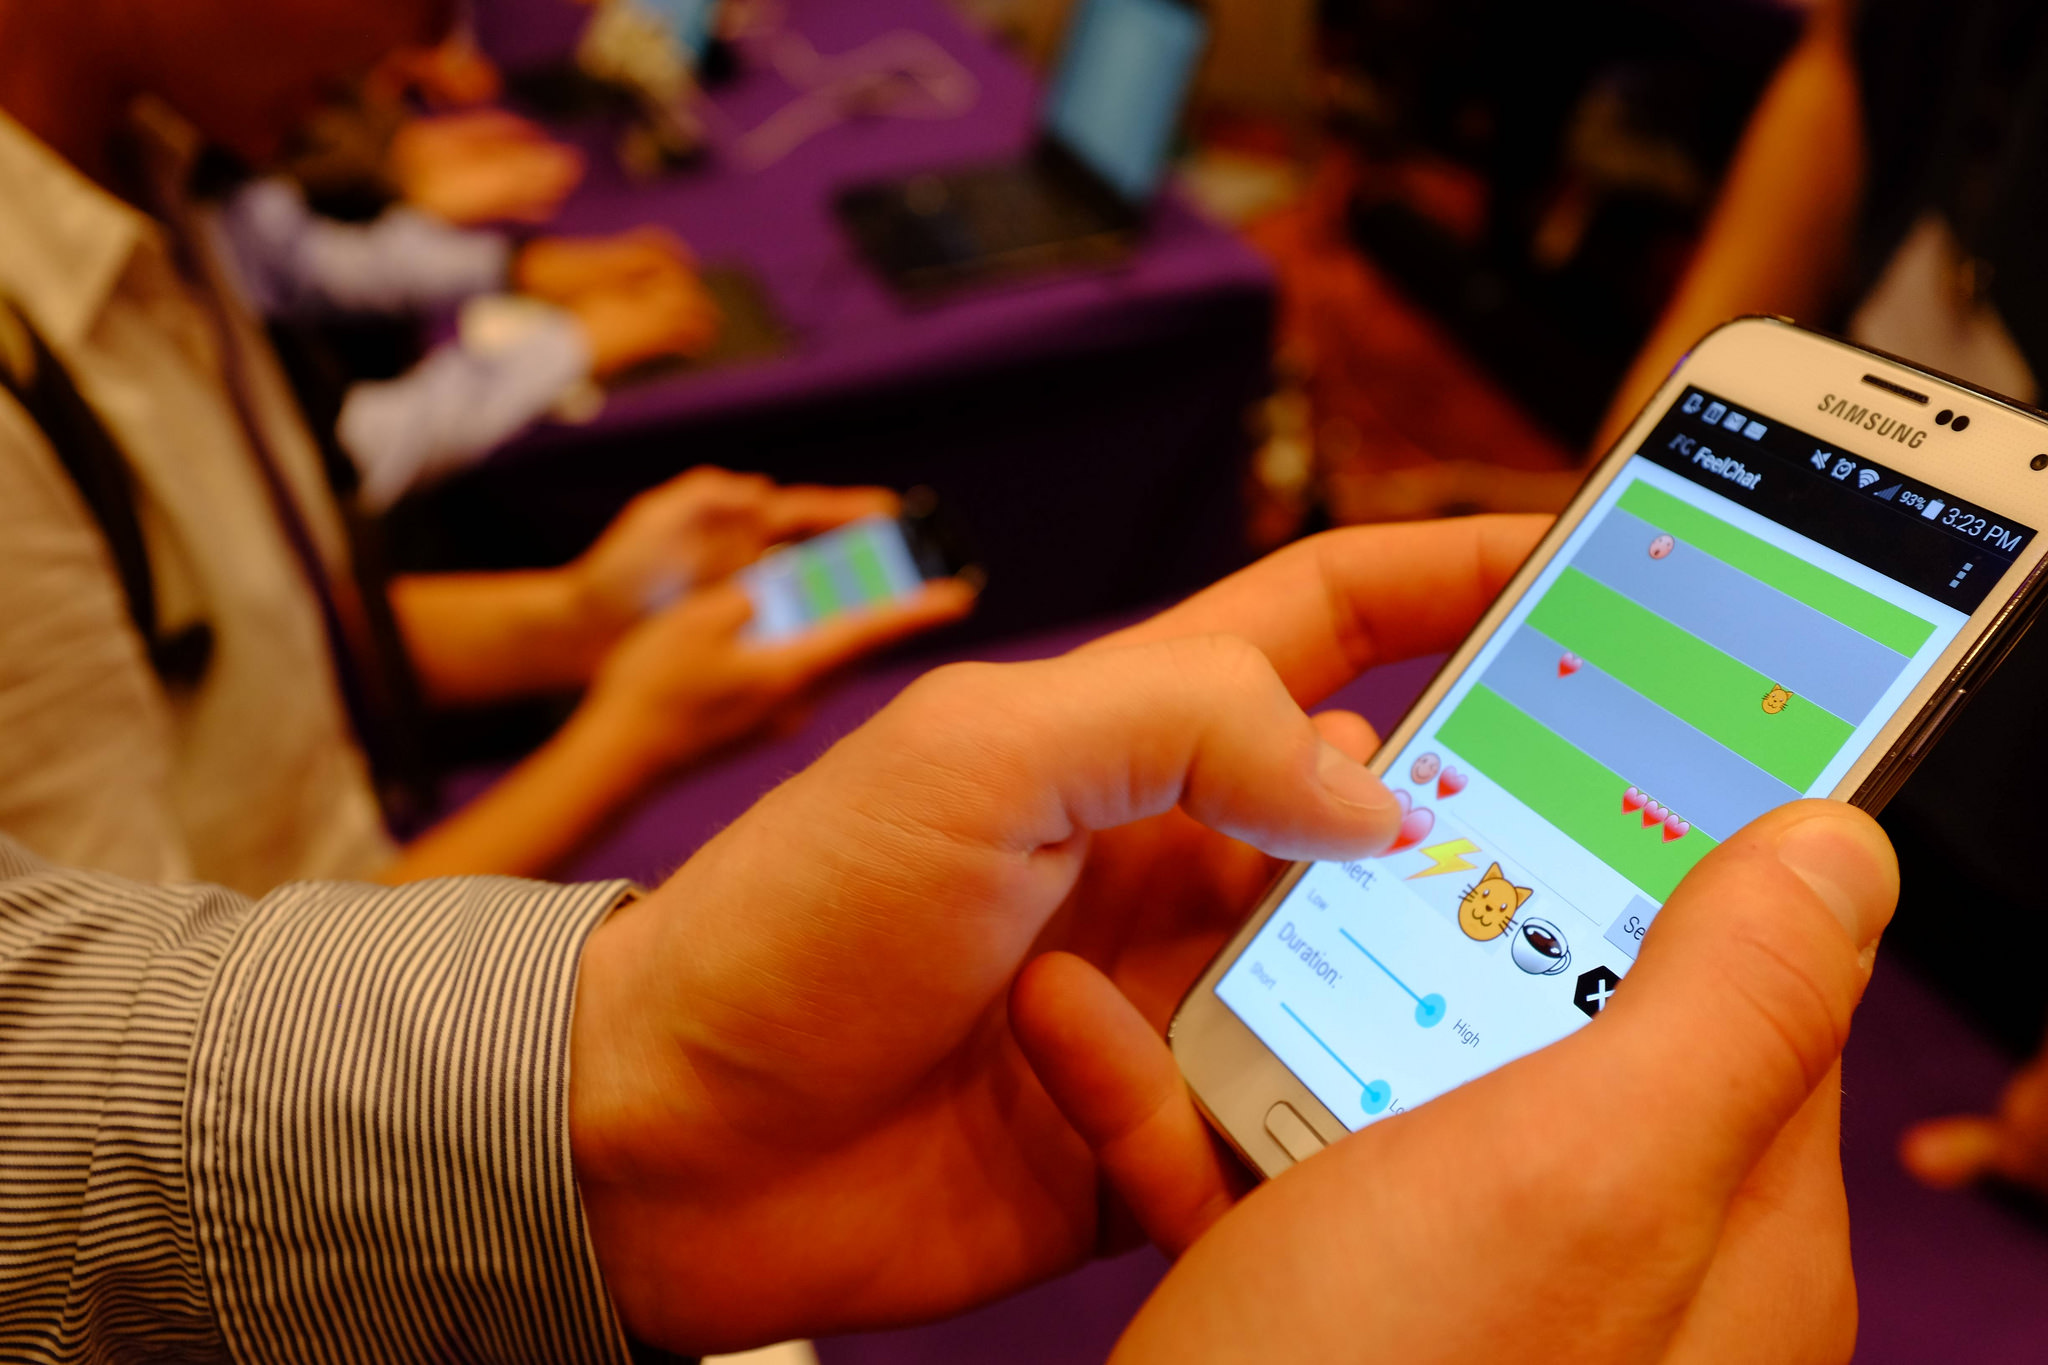
\includegraphics[width=\textwidth]{feelmessenger/FeelMessenger-WHC15} 
   \caption{Implemented Feel Messenger demo at World Haptics 2015.}
   \label{fig:feelmessenger:demo}
\end{figure}

\subsection{Demo}
We developed an Android application on a two Samsung S5 smartphones running Android 4.4.2.
The Android API allows ON/OFF control of the embedded VT motor.
A rough relationship between duty cycle and perceived intensity was determined to create effects.

In this prototype, we explored both predefined effects and Type 1 icons (Feel Effects).
Our predefined effects were designed with 6 emoji.
Our four Type 1 FEs were:
Heartbeat (Pulse FE),
Lightning (Strike FE),
Cat Purr (Motor FE), and
Coffee (Urgency FE).
These VT emoji could be embedded in chat messages, sent between two Android phones using UDP.
VT effects are felt when editing, when received, and when the user taps a message.
All effects were implemented using built-in Android APIs.


\section{RoughSketch: Designing for an Alternative Modality}
\label{sec:applications:roughsketch}

FeelCraft (\autoref{sec:applications:feelcraft}) and Feel Messenger (\autoref{sec:applications:feelmessenger}) used existing infrastructure to conduct VT design, but how do other types of feedback vary?
In Sections \ref{sec:applications:roughsketch} to \ref{sec:applications:cuddlebit}, we investigate other modalities in other applications: programmable friction for touchscreen drawing, force-feedback for education, and affective robots for emotional expression.
Here, in \autoref{sec:applications:roughsketch}, we describe RoughSketch, a drawing application for the TPad Phone.

The TPad Phone (www.thetpadphone.com) is a programmable friction display mounted on an Android phone.
It uses piezo-actuated mechanical vibration to create a cushion of air, reducing friction \cite{Winfield2007}.
As part of the World Haptics 2015 Student Innovation Challenge, we built RoughSketch, a mobile drawing application to explore friction displays for digital mark-making.
We looked at several mark-making interaction techniques including:
\begin{itemize}
    \item \textit{Paintbrush}, where you feel paint leaving your finger,
    \item \textit{Pen and eraser}, based on real-world writing utensils,
    \item \textit{Spray paint}, where you feel the roughness of paint on the screen as you spray,
    \item \textit{Pinch/zoom}, inspired by compressing and stretching rubber, and
    \item \textit{Feel finger}, the ability to feel your drawing on the paper.
\end{itemize}

\begin{figure}[htbp] %  figure placement: here, top, bottom, or page
   \centering
   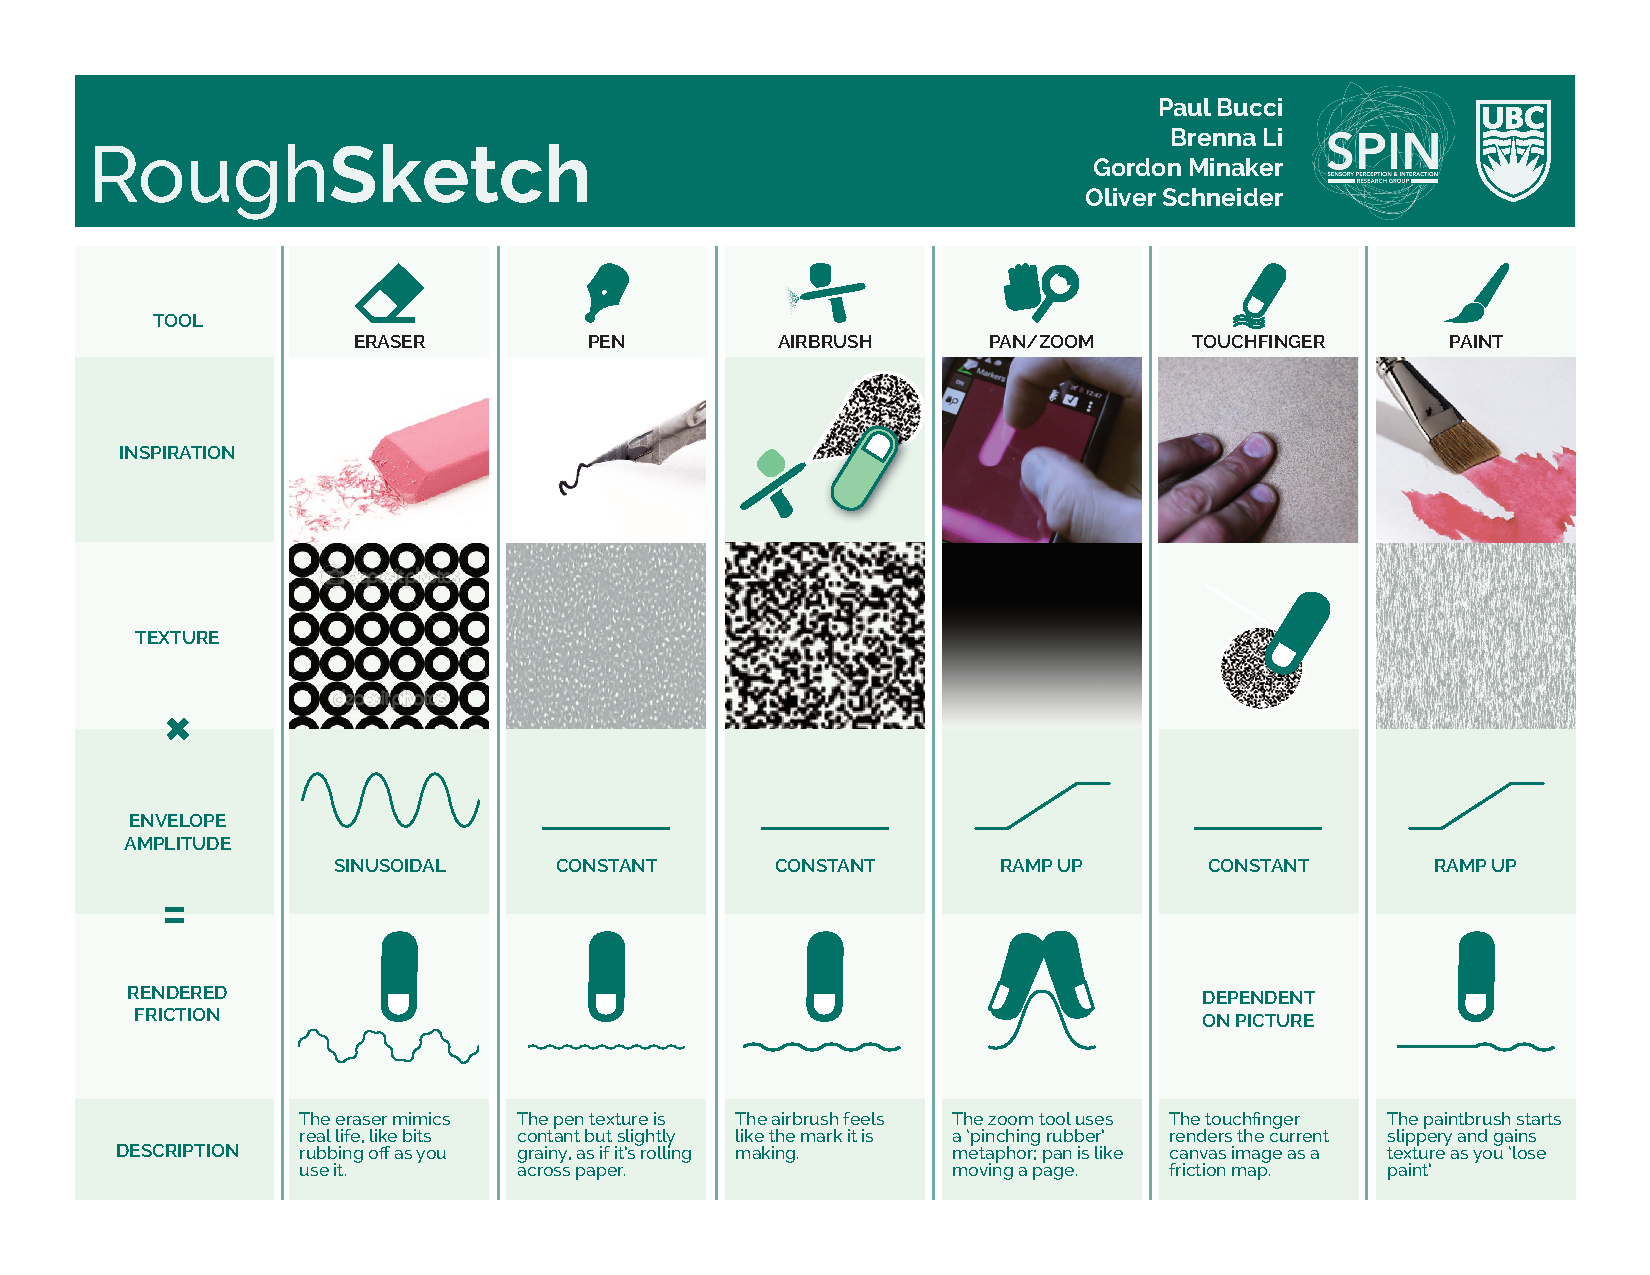
\includegraphics[width=\textwidth]{roughsketch/tpad_handout_final_color} 
   \caption{RoughSketch handout, illustrating interaction techniques an textures.}
   \label{fig:roughsketch:handout}
\end{figure}

\begin{figure}[htbp] %  figure placement: here, top, bottom, or page
   \centering
   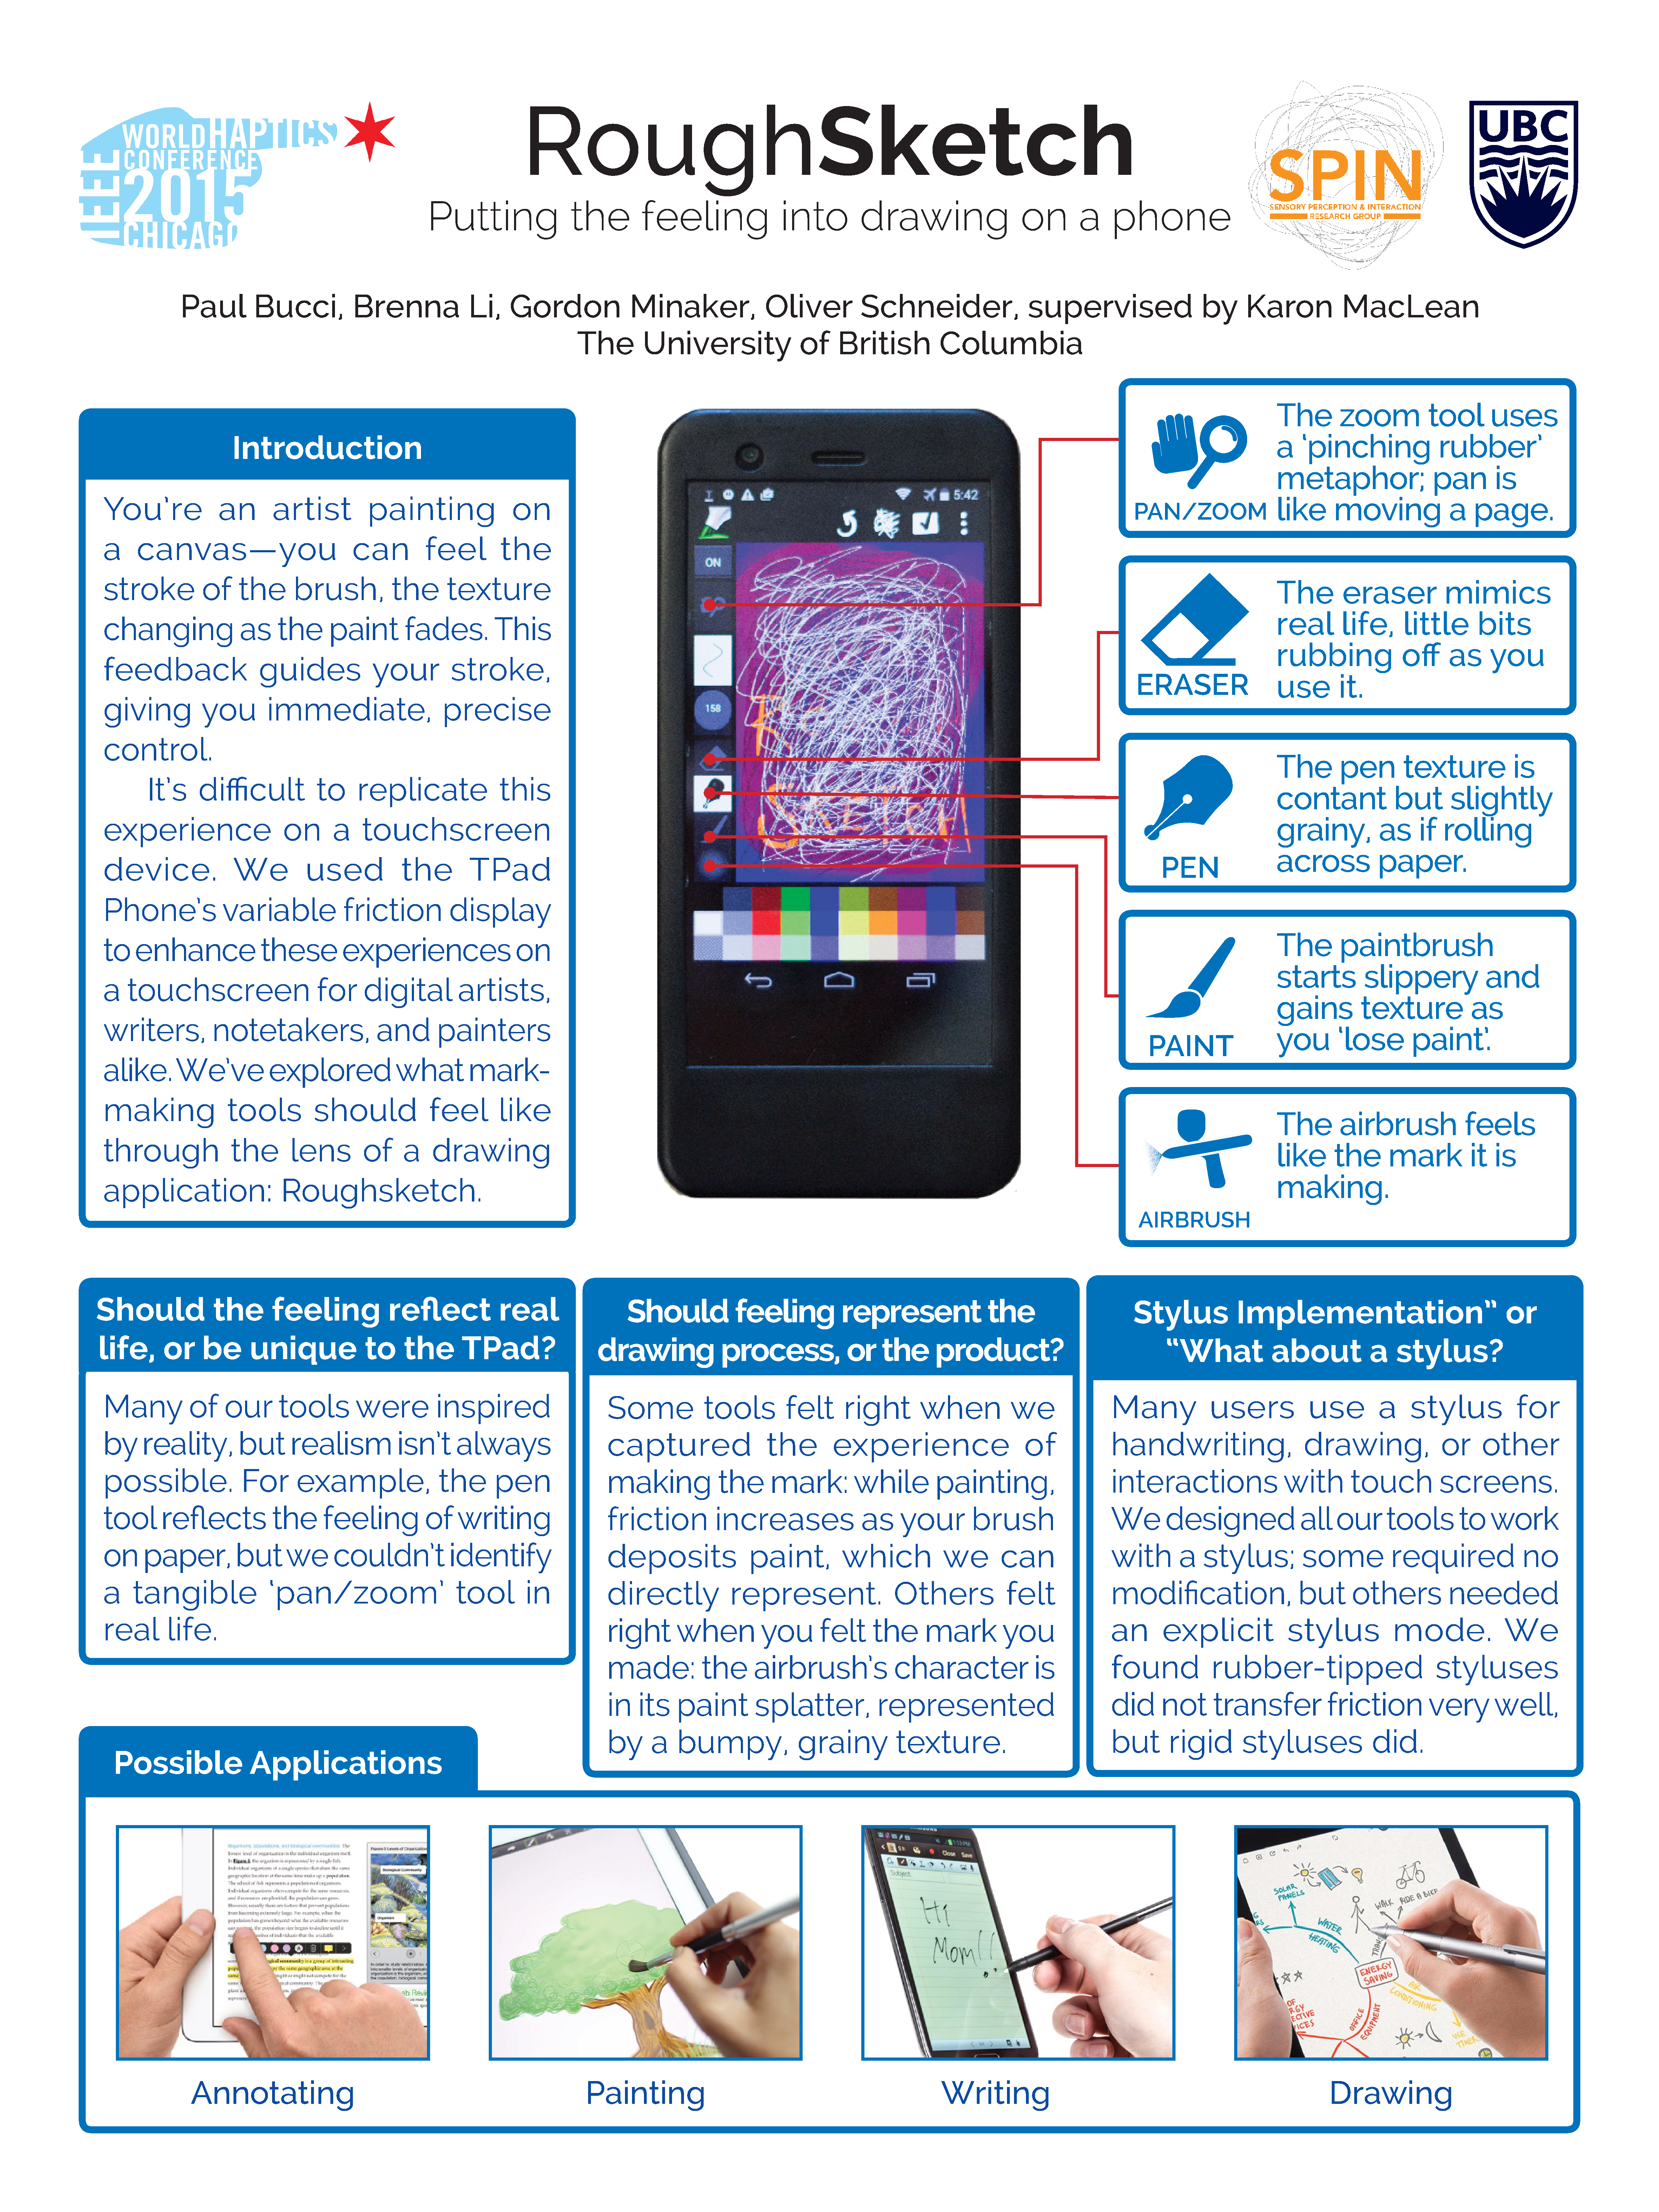
\includegraphics[width=\textwidth]{roughsketch/roughsketch-poster-draft2} 
   \caption{RoughSketch poster, describing interaction techniques and high-level findings.}
   \label{fig:roughsketch:poster}
\end{figure}

\noindent
To implement RoughSketch, we adapted an open-source Android drawing application, Markers (\url{https://github.com/dsandler/markers}) and used the TPad Phone API to control friction using two methods:
static textures defined by bitmaps, and
temporal envelopes that programmatically adapt friction based on input values or time.
We used a variety of real-world metaphors to inspire our designs; these are
illustrated in \autoref{fig:roughsketch:handout}.
While designing and developing RoughSketch, we exposed a design space, finding conflicts for our metaphors, specifically, should TPad sensations feel like their real-world equivalent, or are they unique to the TPad; and 
should rendered textures represent the drawing process, or the finished product?
%We also explored how they would be adapted if the user interacted with RoughSketch using an app rather than their finger.

Our findings are outlined in \autoref{fig:roughsketch:poster}.
In addition to developing different effects, we informally compared haptic feedback to non haptic feedback by including a toggle to friction feedback.
Although some effects were subtle, once disabled, users immediately noticed the difference and preferred to have haptic feedback.
We also explored stylus use, finding that a rubber tip would barely transmit any sensation, while a more rigid tip would propagate the (dampened) effect.




\section{HandsOn: Designing Force-Feedback for Education}
\label{sec:applications:handson}

\begin{figure} [bt]
  \centering
  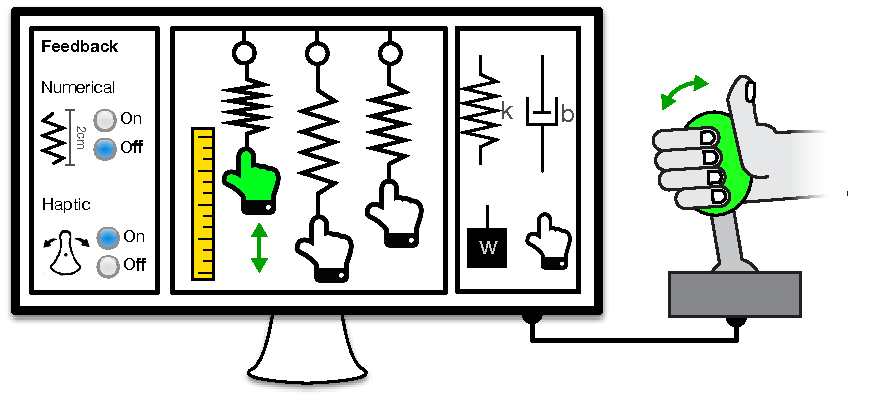
\includegraphics[width=0.7\textwidth]{handson/CyberHap-ConceptualModel-page1_PB_crop}
  \caption{Students, teachers, and researchers can explore science, technology, engineering, and math (STEM) abstractions through low-fidelity haptics, incorporating elements into system designs.}
  % \caption{HandsOn conceptual model:  students, teachers, and researchers can incorporate low-fidelity haptics to learn or design.} 
  % at different levels of exploration.}
  \label{fig:conceptOverview}
\end{figure}

%\inlineHeading{Preface}
In \autoref{sec:applications:handson}, we investigate creative control of 1-degree of freedom (DOF) force-feedback display for education.
Force-feedback is interactive, with output dependent on input, but also controllable when the user holds their hand stationary, unlike programmable friction feedback explored in \autoref{sec:applications:roughsketch}.
The application area, science education, offers important design constraints: feedback must enhance learning without distraction, and in this project, enable creative exploration for students.
We thus both design haptic feedback and enable students to design while they learn.
To manage this, we model feedback as a system of springs, easy to adjust and design, but scalable to more complex tasks by combining multiple springs in series or parallel.


%\subsection{Abstract}
%Embodied, physical interaction can improve learning by making abstractions concrete, 
%while 
%online courses and interactive lesson plans have increased education access and versatility. 
%Haptic technology could integrate these benefits, but requires both low-cost hardware (recently enabled by low-cost DIY devices) and accessible software that enables students to creatively explore haptic environments without writing code.
%To investigate haptic e-learning without user programming, 
%we developed \HandsOn, a conceptual model for exploratory, embodied STEM education software; and implemented it with the \SpringSim interface and a task battery for high school students. 
%%structure graphically presented STEM educational lessons, conveyed through affordable, self-assembled force feedback devices.
%%limits the latter; as such, e-learning haptics has never been evaluated.
%%puts haptic exploration out of reach for most schools or self-learners.
%%We provide this missing \HandsOn, a conceptual model on which we can structure graphically presented STEM educational lessons, conveyed through affordable, self-assembled force feedback devices.
%%
%%a need to write code.
%In two studies, we confirm that low-cost devices can render haptics adequately for this purpose, 
%find qualitative impact of \SpringSim on student strategies and curiosity,
%and identify directions for tool improvement and extension.
%



%Recognition of the value of a hands-on, embodied approach to learning dates to 1907, when
%Maria Montessori opened a school where she used \emph{manipulatives} to teach a wide array of concepts ranging from mathematics to reading, e.g., by introducing the alphabet through children tracing their finger along large, cut-out letters~\cite{Montessori1917}.
%Constructivist learning theories posit that well-designed manipulatives can assist understanding by grounding abstract concepts in concrete representations ~\cite{papert1980,piaget_science_1970},
%%Their use today is 
%and are an accepted core principle in early math and science education, confirmed empirically~\cite{Carbonneau2013}. 
%
%More recently, digital technologies are radically altering learning environments.
%Massive Open Online Courses (MOOCs) expand access, games motivate, and with graphical simulations (e.g., PhET~\cite{wieman_phet:_2008}), students can interact with abstractions to develop their understanding.
%However, these experiences are disembodied. Indirect contact via keyboard, mouse and screen introduces a barrier of abstraction that undermines the connection and path to understanding. 
%% that the interaction aims to promote. 
%
%
%Haptic (touch-based) technology should bring %able to bring
% benefits of physicality and embodied learning~\cite{dourish_where_2004} to interactive virtual environments. 
%It adds a sensory channel as another route to understanding~\cite{calvert_crossmodal_1998}; when deployed appropriately, active exploration can improve understanding~\cite{martin_physically_2005} and memory~\cite{glenberg_activity_2004} of new concepts. 
%Haptic tools have already shown promising results in many specializations, demographics and age groups, both
%to enhance lesson fidelity 
%% (e.g., physics and medical simulations)  -- don't have room for citations!
%and to increase engagement and motivation through tangibility and interactivity; e.g., with devices like Geomagic Touch\footnote{Prev. Sensable Phantom \url{www.geomagic.com/en/products/phantom-omni/overview}}~\cite{williams_implementation_2004} and SPIDAR-G~\cite{sato_haptic_2008}.
%
%Unfortunately, %t
%%These 
%%Sadly, 
%existing approaches have %suffer from 
%both hardware and software limitations.
%Actuated learning tools introduce physical issues of cost, storage, and breakage;
%devices are  too bulky, complex, or expensive for schools or self-learners.
%For software, it is hard for users to construct and explore their own haptic environments. Typically, users load a virtual system to interact with it haptically. This sidelines the rich learning potential of involving users with model construction~\cite{papert1980}.
%We address hardware with the HapKit~\cite{Martinez2016}, a \$50, simple, low-fidelity device constructed from 3d printed materials.  
%
%Our focus here is on software, with a new learning environment that lets users both construct and explore haptic systems. Until now, the only way for a user to construct a haptic system was by programming it herself. Our approach, inspired by Logo ~\cite{papert1980} and Scratch ~\cite{maloney2010}, is to ultimately % KM notes: currently we don't provide much power compared to programming. But it's planned for.
%provide much of the power of a programming language while hiding distracting complexity. 
%
%
%% The rise of open-sourced DIY methods are enabling low-cost, compact, simple designs (e.g., the HapKit \cite{Martinez2016}) which can mitigate these factors, but at the cost of rendering fidelity. 
%% Requirements for display resolution and accuracy are imposed by lessons' perceptual demands, e.g., comparisons needed to assess a hypothesis.
%
%
%
%% \subsubsection{Challenges of Haptic Technology in the Classroom:}
%%
%%  Actuated learning tools introduce obvious physical issues of cost, storage, and breakage. 
%% Devices are often too bulky, complex, or expensive for either schools or self-learners.
%
%% The rise of open-sourced DIY methods are enabling low-cost, compact, simple designs (e.g., the HapKit \cite{Martinez2016}) which can mitigate these factors, but at the cost of rendering fidelity. 
%% Requirements for display resolution and accuracy are imposed by lessons' perceptual demands, e.g., comparisons needed to assess a hypothesis.
%% hypothesis examination and problem solving.
%
%%Unfortunately, hardware is just one layer of the learning experience. 
%%The HapKit, for example, is controlled through an 
%%Arduino\footnote{\url{https://www.arduino.cc}} development environment (IDE). 
%% The problem is not just that 
%%Programming a haptic virtual model is beyond most students in an introductory physics class and thus a massive distraction; worse, procedural programming % , particularly procedural styles, 
%%is a highly abstracted activity that removes  students from the direct-interaction, embodied aspects of the learning environment. 
%
%% Current software that accompanies haptic devices in an educational context can be restrictive \todo{RD: CITE}. An educational haptic-enabled interface must be suitable for immediate interactive use by a broad range of lessons and learners, while supporting engaging educational tasks. %
%% More engaging activities will be creative and design-oriented \rdC{1cite} , building upon more structured introductory exercises; but the coding this eventually entails must remain direct and object-based -- as exemplified by Papert's Logo~\cite{papert1980} and the Scratch visual programming environment~\cite{maloney2010}.
%%
%%Lessons (structured or open-ended) must scale to conventional class sizes, which will be delivered and perhaps designed by teachers themselves non-expert in haptics or programming. 
%
%% \paragraph{Requirements:}  % Note - there's another "requirements" under Apparatus.
%\subsubsection{Approach and Present Objectives:}
\subsection{Introduction}
Recognition of the value of a hands-on, embodied approach to learning dates to 1907, when
Maria Montessori opened a school where she used \emph{manipulatives} to teach a wide array of concepts ranging from mathematics to reading, e.g., by introducing the alphabet through children tracing their finger along large, cut-out letters~\cite{Montessori1917}.
Constructivist learning theories posit that well-designed manipulatives can assist understanding by grounding abstract concepts in concrete representations ~\cite{Papert1980,piaget_science_1970},
%Their use today is 
and are an accepted core principle in early math and science education, confirmed empirically~\cite{Carbonneau2013}. 
More recently, digital technologies are radically altering learning environments.
Massive Open Online Courses (MOOCs) expand access, games motivate, and with graphical simulations (e.g., PhET~\cite{wieman_phet:_2008}), students can interact with abstractions to develop their understanding.
However, these experiences are disembodied. Indirect contact via keyboard, mouse and screen introduces a barrier of abstraction that undermines the connection and path to understanding. 
% that the interaction aims to promote. 


Haptic (touch-based) technology should bring %able to bring
 benefits of physicality and embodied learning~\cite{dourish_where_2004} to interactive virtual environments. 
It adds a sensory channel as another route to understanding~\cite{calvert_crossmodal_1998}; when deployed appropriately, active exploration can improve understanding~\cite{martin_physically_2005} and memory~\cite{glenberg_activity_2004} of new concepts. 
Haptic tools have already shown promising results in many specializations, demographics and age groups, both
to enhance lesson fidelity 
% (e.g., physics and medical simulations)  -- don't have room for citations!
and to increase engagement and motivation through tangibility and interactivity; e.g., with devices like Geomagic Touch\footnote{Prev. Sensable Phantom \url{www.geomagic.com/en/products/phantom-omni/overview}}~\cite{williams_implementation_2004} and SPIDAR-G~\cite{sato_haptic_2008}.

Unfortunately, %t
%These 
%Sadly, 
existing approaches have %suffer from 
both hardware and software limitations.
Actuated learning tools introduce physical issues of cost, storage, and breakage;
devices are  too bulky, complex, or expensive for schools or self-learners.
For software, it is hard for users to construct and explore their own haptic environments. Typically, users load a virtual system to interact with it haptically. This sidelines the rich learning potential of involving users with model construction~\cite{Papert1980}.
We address hardware with the HapKit~\cite{Martinez2016}, a \$50, simple, low-fidelity device constructed from 3d printed materials.  

Our focus here is on software, with a new learning environment that lets users both construct and explore haptic systems. Until now, the only way for a user to construct a haptic system was by programming it herself. Our approach, inspired by Logo ~\cite{Papert1980} and Scratch ~\cite{maloney2010}, is to ultimately % KM notes: currently we don't provide much power compared to programming. But it's planned for.
provide much of the power of a programming language while hiding distracting complexity. 


% The rise of open-sourced DIY methods are enabling low-cost, compact, simple designs (e.g., the HapKit \cite{Martinez2016}) which can mitigate these factors, but at the cost of rendering fidelity. 
% Requirements for display resolution and accuracy are imposed by lessons' perceptual demands, e.g., comparisons needed to assess a hypothesis.



% \subsubsection{Challenges of Haptic Technology in the Classroom:}
%
%  Actuated learning tools introduce obvious physical issues of cost, storage, and breakage. 
% Devices are often too bulky, complex, or expensive for either schools or self-learners.

% The rise of open-sourced DIY methods are enabling low-cost, compact, simple designs (e.g., the HapKit \cite{Martinez2016}) which can mitigate these factors, but at the cost of rendering fidelity. 
% Requirements for display resolution and accuracy are imposed by lessons' perceptual demands, e.g., comparisons needed to assess a hypothesis.
% hypothesis examination and problem solving.

%Unfortunately, hardware is just one layer of the learning experience. 
%The HapKit, for example, is controlled through an 
%Arduino\footnote{\url{https://www.arduino.cc}} development environment (IDE). 
% The problem is not just that 
%Programming a haptic virtual model is beyond most students in an introductory physics class and thus a massive distraction; worse, procedural programming % , particularly procedural styles, 
%is a highly abstracted activity that removes  students from the direct-interaction, embodied aspects of the learning environment. 

% Current software that accompanies haptic devices in an educational context can be restrictive \todo{RD: CITE}. An educational haptic-enabled interface must be suitable for immediate interactive use by a broad range of lessons and learners, while supporting engaging educational tasks. %
% More engaging activities will be creative and design-oriented \rdC{1cite} , building upon more structured introductory exercises; but the coding this eventually entails must remain direct and object-based -- as exemplified by Papert's Logo~\cite{papert1980} and the Scratch visual programming environment~\cite{maloney2010}.
%
%Lessons (structured or open-ended) must scale to conventional class sizes, which will be delivered and perhaps designed by teachers themselves non-expert in haptics or programming. 

% \paragraph{Requirements:}  % Note - there's another "requirements" under Apparatus.
\subsubsection{Approach and Present Objectives:}
To study \textit{how} to unlock the potential of hapticized virtual environments in STEM education, we need a viable front-end.
%
% Here, we take the first step towards these requirements with a graphical learning interface which presents a \textit{single} lesson as an evaluation instrument with several purposes. It must allow us to 
%
To this end, we first established a \textit{conceptual model} (\HandsOn):
central interface concepts, supported operations and language  \cite{johnson_conceptual_2002} that can be employed in a broad range of lessons involving physical exploration and design. 

Next, we implemented the \HandsOn conceptual model (CM) in \SpringSim, a first-generation learning interface prototype narrowly focused in a module on mechanical springs and targeted at high school physics students.
To render forces we used the HapKit, a simple device with a 3D-printable handle providing affordable, self-assembled 1 DOF force-feedback for about \$50 USD.
%
As an evaluation instrument, this single-lesson implementation allows us to 
(a) measure a given hardware platform's fidelity for a representative perceptual task; 
(b) attain insight into the kinds of lessons such a system can  leverage; and
(c) assess its learning-outcome efficacy relative to conventional methods.
With these answers, we will be able to design a more powerful tool.

We report results from two user studies: 
(1) the HapKit's ability to display differentiable springs with and without graphical reinforcement, and 
(2) a qualitative evaluation of \SpringSim for a carefully designed set of  educational tasks.
We confirm that the \SpringSim interface and its conceptual model \HandsOnCM %substantively supported physical feedback in these tasks, 
%We confirmed that the \SpringSim interface and its conceptual skeleton  \HandsOnCM incorporate physical forces substantively into these tasks, 
%and \osE{compared input device use (mouse vs. HapKit)}.
%investigated the comparative use of mouse versus Hapkit as input devices. 
are understandable and usable, 
%We report our findings on participants' comprehension of the CM, 
describe the role of haptics compared to mouse input, and
%Finally, we 
provide %guidance and
recommendations
for future evaluation, lesson and tool design.

% ============================================
\subsection{Tool Development: Conceptual Model and Interface}
Our goal was to find a software model to use and evaluate low-cost force feedback in an educational setting.
We began by choosing a device, establishing requirements, and exploring capabilities through use cases and prototypes.
From this, we defined %a conceptual model, 
\HandsOn.
We then implemented  essential features in a medium-fidelity prototype, \SpringSim, for our user studies.

% % \subsubsection{Overview:}
% We developed \HandsOn as a conceptual framework for educational software tools providing a flexible, exploratory front-end to an accessible, 1-DOF haptic device such as the Hapkit. 

% We followed the following design process.
% Requirements gathered from educators and students fed extensive iteration on a extensible underlying conceptual model (CM -- the core concepts and operations supported by the tool, and their representation to the user), around which we implemented a medium fidelity prototype. 
% % \springSim's CM is capable of supporting educational lesson plans beyond its current implementation. 
% Currently, \SpringSim includes one lesson module in which students can explore properties of springs and spring systems.
% In future implementations, its comprehensive CM can support more complex and abstract education topics, such as lessons on electrical circuits or trigonometry.


\subsubsection{Initial design (requirements):}
We established six guiding requirements. % for our model.
%Early piloting motivated and suggested an approach for an exploratory interface structured within a lesson plan. 
First, we developed initial prototypes with HapKit 2.0
through two pilot studies with middle school students (described in \cite{Martinez2016}).
These highlighted two aspects of a practical, accessible approach for junior students: 1) no programming; instead 2) a graphical implementation of an exploratory interface within a lesson plan.
%These established 1) a confirmation that programming provided significant barriers to students, and 2) that graphical interfaces were most practical as an exploratory interface within a lesson plan.
%While we first planned for open-ended design tasks to promote engagement, we here realized that a single structured lesson focused on a small number of tangible concepts was more appropriate for future comparative evaluation of the haptic feedback's educational utility. 
We also needed to build on known benefits of traditional classroom practices, and enable learning-outcome comparison.
% came from previous interfaces and features of using a haptics.
We must 3) 
support the same \textit{types} of traditional education tasks, e.g., let students  compare and assemble spring networks as easily as in a hands-on physics lab; 
but also 4) \textit{extend} them, to leverage the flexibility offered by a manipulative that is also virtual.
Similarly, to support future formal comparisons, %to pursue inquiry into the learning benefit of haptics,
%, we need to assess the learning benefit added by rendered forces to an educational simulation over the  graphics-based status quo. 
our model needs to 5) support both haptic and non-haptic (mouse) inputs.
Finally, to ensure generality we also needed to 6) support diverse STEM topics, like physics, biology, and mathematics.
Further design yielded a model that addressed these requirements: \HandsOn.
% This model had to work both with Hapkit, and without it. 
% Subsequent low-fidelity prototyping around these constraints yielded a conceptual model based on exploration: \HandsOn.

% From this we established initial requirements:
% We assessed interface requirements during pilot studies and classroom visits in collaboration with education researchers  and
% iteratively with low-fidelity prototyping (paper and software mockups) which were evaluated informally both with team members and representative students, % GM, for the students I'm thinking the middle school studies. Legit to say this?
% This culminated in a CM and then a medium fidelity prototype of the spring simulation element. \SpringSim with HapKit (fully functional but minimally featured, with simply rendered but carefully planned screen elements) was piloted with volunteers, and iterated once more prior to formal evaluation.
%to conduct comparative studies that more closely investigate Hapkit's utility. 
% Our initial evaluation-platform lesson had to expose insight into user preferences for and strategies in using haptic support in an education task.

% \paragraph{Process:}
% Tool design was preceded by and then intertwined with educational task design, both taking input from education researchers. We considered and even prototyped a broad set of candidate domains, learning goals and task style (e.g., structured versus open-ended) before  realizing that a first ``studyable'' lesson must be relatively simple and structured, and focusing on spring simulation. 



% -----------------------------
\subsubsection{Conceptual Model:}%: \HandsOn.}

%02.07 BEGIN NEW CM SECTION
%Our conceptual model (CM) is primarily based on our first two requirements (R1 \& R2):
%\gmC{Noticing that we don't go through all of R1-R6 in this section. Not sure if its necessary?}
\HandsOn is a programming-free (R1) graphical interface supporting learner exploration (R2), with a number of key \emph{concepts}: \textit{Interactive Playground}, \textit{Hands}, \textit{Design Palette}, \textit{Objects}, \textit{Properties}, \textit{Haptic} and \textit{Visual Controls}.
Exploration is supported at various levels (Figure~\ref{fig:conceptObjects}).

\begin{figure} [b]
  \centering
  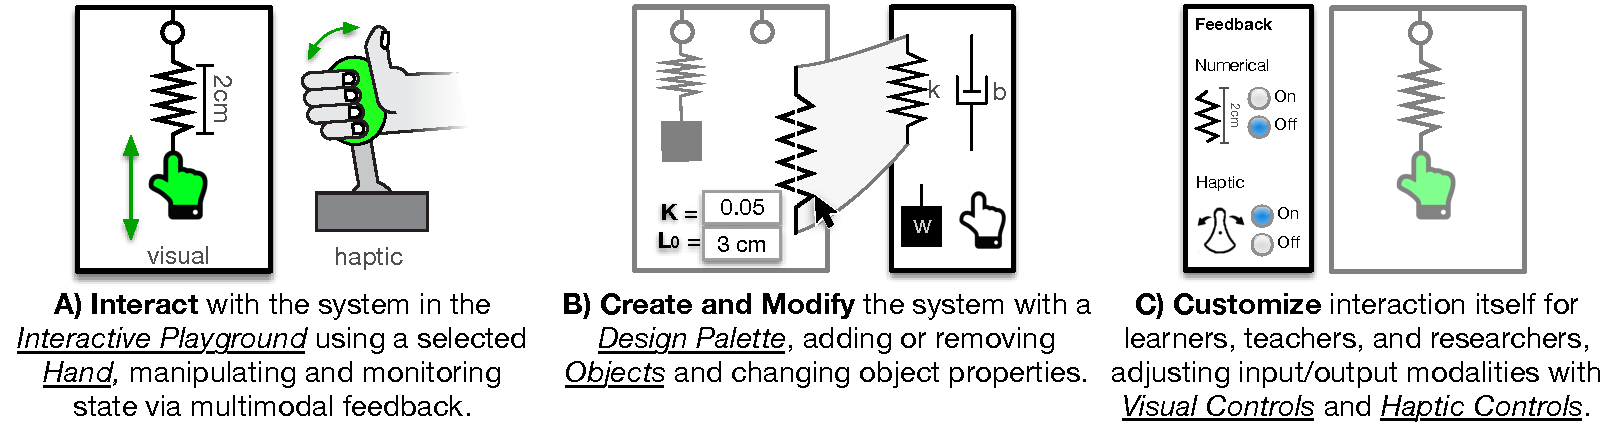
\includegraphics[width=\textwidth]{handson/CyberHap-ConceptualModel-2016-02-08b}
  \caption{The \HandsOn CM enables three kinds of exploration based on requirements.}
  \label{fig:conceptObjects}
\end{figure}

%``How does it feel to interact with a spring-mass-damper system?''
The \emph{Interactive Playground} provides a virtual sandbox where
users can interact with virtual environments (VE). % using \emph{Hands}. 
\emph{Hands} allow users to select, move, and manipulate components in the Interactive Playground. %The \emph{Hands} can be
Control occurs with either the mouse or a haptic device to receive force-feedback (Figure~\ref{fig:conceptObjects}A) (R5). In the design and modification phase, users can add or remove \emph{objects} like springs, masses, gears, or electrons by dragging them to and from a \emph{Design Palette} (R3). Once added to the scene, users can modify their physical properties (e.g., a spring constant k) and make changes to the VE (Figure~\ref{fig:conceptObjects}B). After construction, the user can customize their interaction with their VE by adjusting \emph{Visual Controls} and \emph{Haptic Controls} options that extend interactions in new ways afforded by haptics (R4) (Figure~\ref{fig:conceptObjects}C). Because of the flexibility afforded by having multiple \emph{objects} in the playground with multiple \emph{Hands} for interaction points, and customization of interaction and feedback, \HandsOn can support different STEM topics (R6), from biology to mathematics.
To confirm the viability of this approach, we built an initial prototype with essential features: \SpringSim.


%Most essentially, users simply interact with a virtual system in the \emph{Interactive Playground}, receiving feedback, e.g., from manipulating a spring-mass-damper system and feeling and seeing state like output forces (Figure~\ref{fig:conceptObjects}A). %``How does it feel to interact with a spring-mass-damper system?''
%A \emph{Hand} is the boundary between real and virtual spaces (what the user is currently feeling and manipulating).
%\emph{Hands} allowing users to interact with different parts of a system by being \underline{selected}, \underline{moved} (e.g., stretched), \underline{connected} \osC{?} and the result \underline{measured} -- e.g., in the context of a lesson plan, a learner can use a ruler object to  measure spring displacement to understand stiffness.
%Based on previous educational interfaces (R3), we also include the ability to add  or remove \emph{objects} to a structure to create new scenarios, and modify properties, e.g., adding a new mass to a system.
%This is analogous to students trying different spring systems in a physics lab, or modifying simulations in PhET \cite{wieman_phet:_2008}.
%In \HandsOn, this is done through a \emph{design palette}, a set of possible objects and operations to modify them (Figure~\ref{fig:conceptObjects}B).

%To understand how to extend possible interaction in new ways afforded by haptics (R4), we include customization controls for interaction feedback: \textit{Visual Controls} and \textit{Haptic Controls} (Figure~\ref{fig:conceptObjects}C).
%Learners, teachers, and researchers can change
%``How does it feel when you add a spring to a mass, and change the mass/spring ratio?''
%Finally, they can customize
%\textit{how} interaction happens, e.g., toggling display modalities or increasing force gain.
%This also enables comparison between haptic and non-hapti
%c controls (R5), possible through \emph{Hands}, which can be represent a 1-DOF force-feedback device or a standard computer mouse.
%Because of the flexibility afforded by having multiple \emph{objects} in the playground with multiple \emph{Hands} for interaction points, and customization of interaction and feedback, \HandsOn can support different STEM topics (R6), from biology to mathematics.
%To confirm the viability of this approach, we built an initial prototype with essential features: \SpringSim.

%We included interaction customization for experiment control, but later realized this feature has learning uses. 


% You can 
% 1) Interact with model: manipulate its state, i.e. providing input and receiving feedback (stretch spring, feel its force, drag ruler to measure the springs). Objects: Hand, Springs, Ruler,  - the hand.
% 2) Modify model: edit/design the model (which springs, how connected, their K-constants)
% 3) Modify interaction itself - e.g., mapping from input to output, gain of haptic feedback (including off), what parameters you can see visually. Originally for development purposes, may be useful for teachers or even students later (ind. differences).


% \HandsOn includes a small number of key  \textit{concepts}. 
% A selected \textit{Hand} is the boundary between real and virtual spaces (what the user is currently feeling and manipulating).  
% \textit{Objects} (e.g., virtual springs and masses, and measurement tools)   have \textit{Object Properties} (e.g., stiffness constant and weight).
% In an \textit{Interactive Playground}, \textit{Objects} can be (via the active \textit{Hand}) \underline{selected}, \underline{moved} (e.g., stretched), \underline{connected} and the result \underline{measured} -- e.g., in the context of a lesson plan, a learner can use a ruler object to  measure spring displacement to understand stiffness. 
% When the object attachment is moved with the \textit{Hand}, the virtual model is recomputed and the resultant model force at that point displayed through the haptic device, if present and turned on.
% % A \textit{Design Palette} provides these operations (e.g., with an object creator and/or a property editor).
% A \textit{Design Palette} is a source of new objects for the playground and editing mechanisms for existing objects. 
% % The graphic and haptic objects have a small number of low-level parameters accessible through the \textit{Visual Controls} and \textit{HapKit Controls} boxes.

% %This exploration is meant to happen within 
% The \HandsOn model extends naturally to many complex lesson domains explored in prototyping, including physical systems, chemistry, and biology.


%
% 02.07 BEGIN OLD CM SECTION
%
% At the highest level, our CM supports exploration at varying levels of initiative (Figure~\ref{fig:conceptObjects}). 
% Most essentially, users simply interact with a model, receiving feedback: ``How does it feel to interact with a spring-mass-damper system?''
% Next, they can add  objects to a structure to create new scenarios, and modify properties: 
% ``How does it feel when you add a spring to a mass, and change the mass/spring ratio?''
% Finally, they can customize \textit{how} interaction happens, by enabling or adjusting input and output (e.g., control/display  or  force gain).
% We included interaction customization for experiment control, but later realized this feature has learning uses. 

% \begin{figure} [b]
%   \centering
%   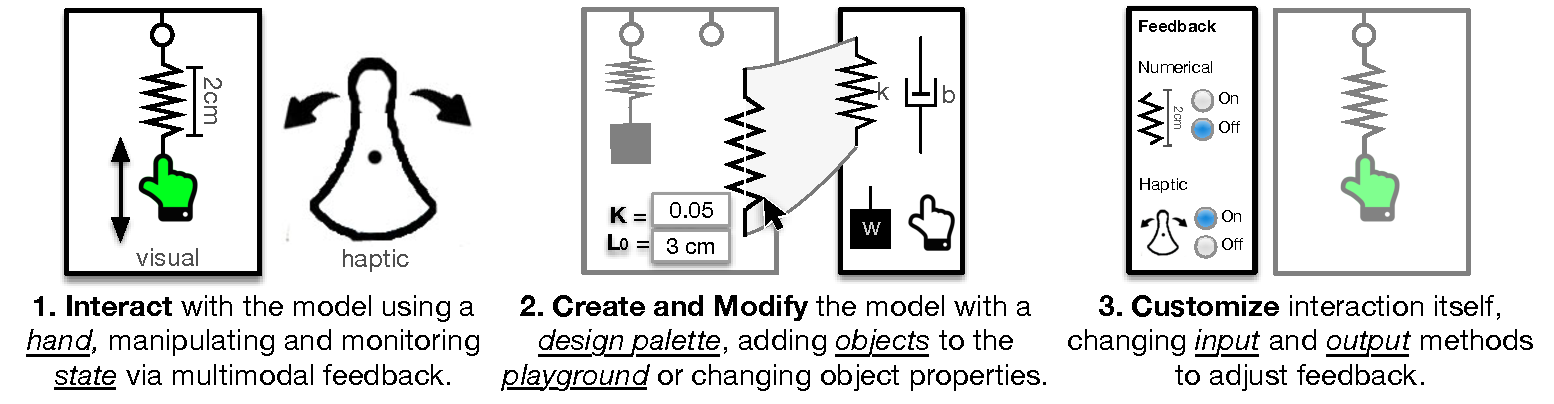
\includegraphics[width=1.05\textwidth]{CyberHap-ConceptualModel-sketch}
%   \caption{HandsOn conceptual model.}
%   \label{fig:conceptObjects}
% \end{figure}
% % You can 
% % 1) Interact with model: manipulate its state, i.e. providing input and receiving feedback (stretch spring, feel its force, drag ruler to measure the springs). Objects: Hand, Springs, Ruler,  - the hand.
% % 2) Modify model: edit/design the model (which springs, how connected, their K-constants)
% % 3) Modify interaction itself - e.g., mapping from input to output, gain of haptic feedback (including off), what parameters you can see visually. Originally for development purposes, may be useful for teachers or even students later (ind. differences).


% \HandsOn includes a small number of key  \textit{concepts}. 
% A selected \textit{Hand} is the boundary between real and virtual spaces (what the user is currently feeling and manipulating).  
% \textit{Objects} (e.g., virtual springs and masses, and measurement tools)   have \textit{Object Properties} (e.g., stiffness constant and weight).
% In an \textit{Interactive Playground}, \textit{Objects} can be (via the active \textit{Hand}) \underline{selected}, \underline{moved} (e.g., stretched), \underline{connected} and the result \underline{measured} -- e.g., in the context of a lesson plan, a learner can use a ruler object to  measure spring displacement to understand stiffness. 
% When the object attachment is moved with the \textit{Hand}, the virtual model is recomputed and the resultant model force at that point displayed through the haptic device, if present and turned on.
% % A \textit{Design Palette} provides these operations (e.g., with an object creator and/or a property editor).
% A \textit{Design Palette} is a source of new objects for the playground and editing mechanisms for existing objects. 
% % The graphic and haptic objects have a small number of low-level parameters accessible through the \textit{Visual Controls} and \textit{HapKit Controls} boxes.

% %This exploration is meant to happen within 
% The \HandsOn model extends naturally to many complex lesson domains explored in prototyping, including physical systems, chemistry, and biology.

%
% 02.06 END OLD CM section
%


% Spring generator is PART of the design palette (only part for SpringSim) \\
% Design palette includes both spring generator (right) spring properties (left) and deletion. Modfy AND design -


% Possible \textit{operations} on these object are revealed by key screen elements (Figure~\ref{fig:conceptOperations}): 

%
% \begin{figure} [bt]
%   \centering
%   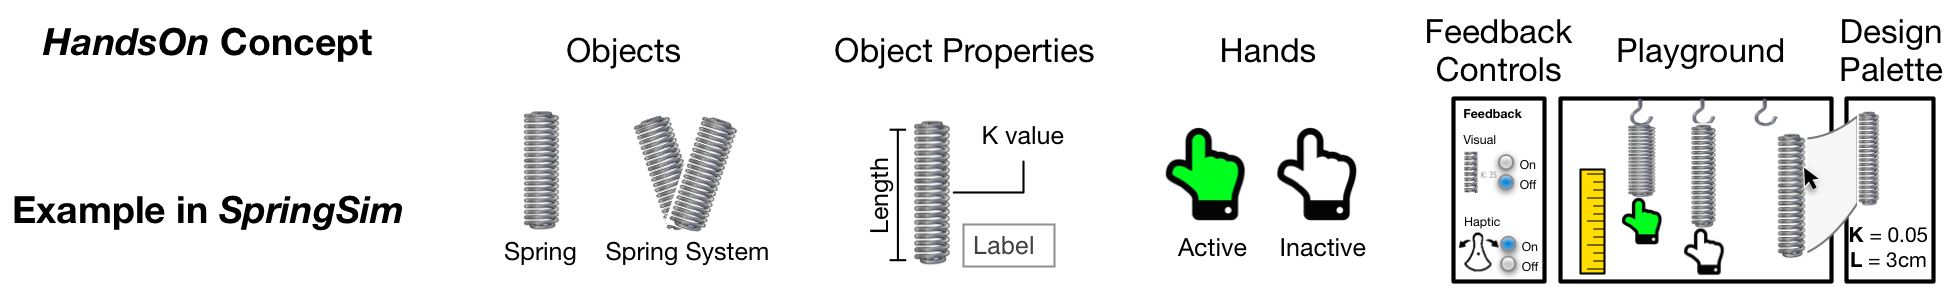
\includegraphics[width=\textwidth]{CyberHap-CM-2}
%   \caption{\todo{add caption}}
%   \label{fig:conceptObjects}
% \end{figure}
% %
% \begin{figure} [bt]
%   \centering
%   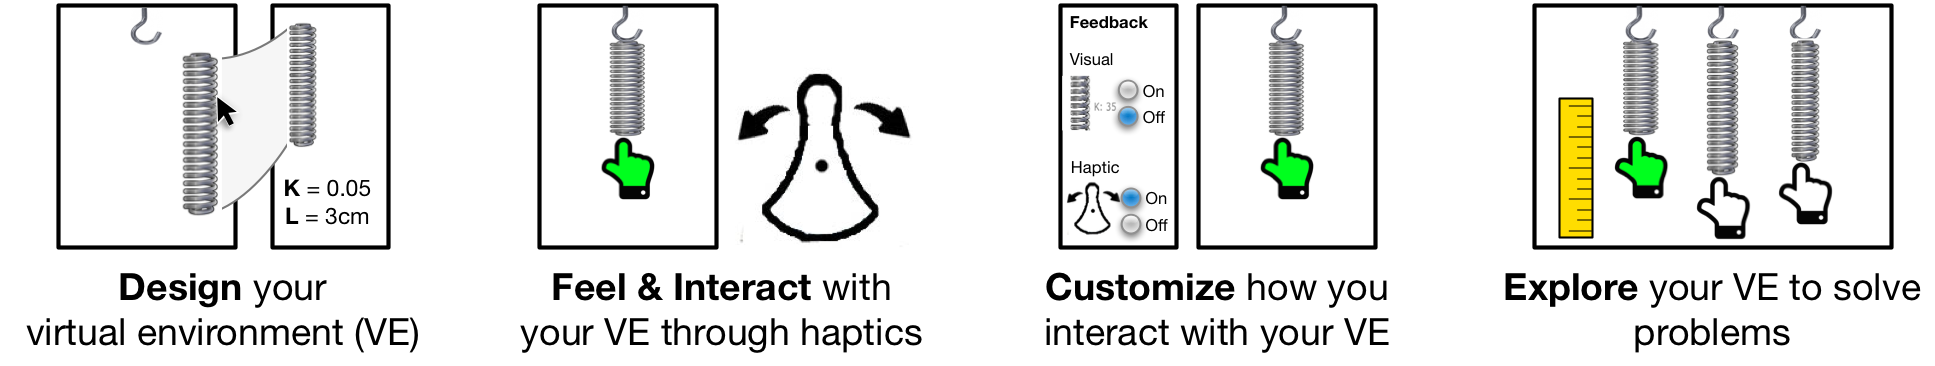
\includegraphics[width=\textwidth]{CyberHap-CM-1}
%   \caption{\todo{add caption}}
%   \label{fig:conceptOperations}
% \end{figure}


% \paragraph{SpringSim Prototype Implementation}
% In this first instantiation, \SpringSim is a principally a tool for education researchers to compare novel educational strategies and utility to conventional alternatives. We therefore technically support both HapKit and mouse as input devices. 
% This model had to work both with Hapkit, and without it. 
% Note: GM says this version has amplified screen controls - for experimenter use. E.g. turning hapkit on/off, but it might also be helpful for students exploration, and/or teachers. 

% -----------------------------
\subsubsection{Implemented Prototype: }
Our first \HandsOn interface is \SpringSim
(Figure~\ref{fig:springsim}),
%We chose springs systems for our proof-of-concept implementation 
which supports  a spring lesson -- spring systems are natural as a virtual environment of
 easily-controlled complexity. 
%(from single springs to a serial or parallel assembly), 
%allowing the user to create and
%interact with a wide variety of
%configurations.
%for scalable task difficulty; a set of tasks of escalating challenge can be built around them; and they
%
%
%
%
%
\begin{figure} [bt]
   \centering
   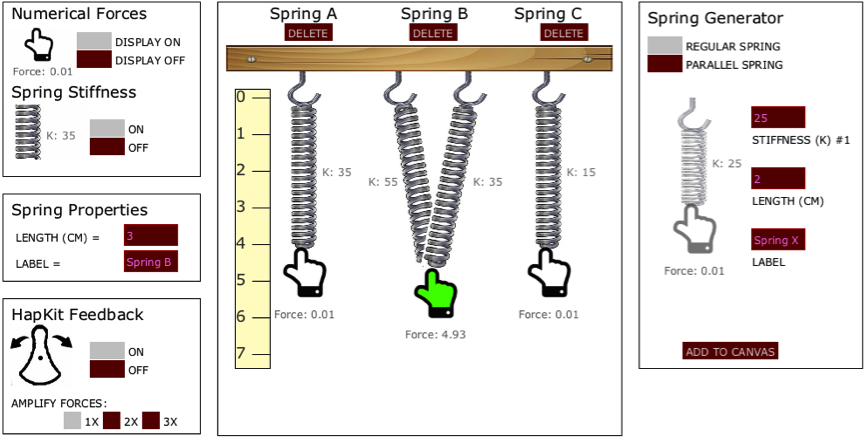
\includegraphics[width=0.9\textwidth]{handson/SpringSim-cropped}
   \caption{\SpringSim interface, a \HandsOn sandbox for a single lesson module on springs.}
   \label{fig:springsim}
\end{figure}
In \SpringSim, \emph{objects} include single springs and parallel spring systems, with properties
%In \SpringSim, 
% users can choose a single spring or build a parallel spring system, and for each element, specify a stiffness value (N/m), rest length (cm) and label.
%users interact with spring \textit{Objects} using \textit{Hands} in the \textit{Interactive Playground},
%and can update
spring rest length (cm), stiffness (N/m) and label.
The \emph{Design Palette} includes the \textit{Spring Properties} and \textit{Spring Generator} UI components.
Implemented \emph{Visual Controls} are toggling numerical displays of spring stiffness and force; \emph{Haptic Controls}  toggle HapKit feedback and output amplification. The open-source repository for SpringSim is available at https://github.com/gminaker/SpringSim.
%They can add, combine (into parallel assemblies), delete and measure springs at rest or deflected.
%
 %Adjusting haptic feedback gain, and which information is displayed in a visual format (e.g., spring constants, and numerical value of the force exerted by the \textit{Hands}) are additional ways to observe spring dynamics.





% \begin{itemize}
%     \item Task 1: Rank three springs in order from least to most stiff
%     \item Task 2: Plot the relationship between displacement and force for two springs.
%     \item Task 3: Estimate the stiffness of an unknown spring, given two reference springs with known stiffness value. 
%     \item Task 4: Predict the behaviour of springs in parallel. 
%     \item Task 5: Design a parallel spring system that uses two springs to behave like an individual spring of stiffness 55 n/m.
%     \item Task 6: Predict the behaviour of springs in series. 
%     \item Task 7: Describe any relationships you have noticed between spring force, displacement, and stiffness.
% \end{itemize}

% \section{Evaluation of SpringSim for Perceptual Transparency and Usability}

% We conduct two studies of our medium fidelity \SpringSim\ prototype. 
% First, we conduct a perceptual study to characterize the perceptibility of SpringSim and Hapkit; specifically designed to validate a students’ ability to distinguish between pre-selected springs that would be used in our second user study. Current literature does provided some insight on perceptual properties of computer-controlled actuators \cite{jones_1990}, however, the perceptual properties of springs rendered virtually on the HapKit have yet to be fully characterized. Additionally, current literature describes the human ability to resolve force and compliance of springs (\gmC{TODO: CITE}), however, we were unable to find literature that considers both the virtual rendering and visualization of springs, as is the case with SpringSim and Hapkit.

% Following the completion of our perceptual study, user studies were conducted on students to investigate (a) the usability of SpringSim, (b) the effectiveness of our designed educational tasks for investigating haptics-based educational intervention studies in future work, and (c) provide preliminary insights into the effect of Hapkit on students’ educational strategies. 

\subsection{Study 1: Perceptual Transparency}
Before evaluating \SpringSim, we needed to confirm that the HapKit could render spring values sufficiently for our qualitative analysis.
%Our goal was to identify spring values that were distinguishable to ensure our Study 2 results were not overwhelmed by perceptual failures of the device.

\subsubsection{Methods:}

14 non-STEM undergraduate students (8 females) participated in a two-alternative, forced choice test with two counterbalanced within-subject conditions:
%Participants completed an entrance survey before being presented with pre-selected spring pairs across two counterbalanced conditions:
\textit{HapKit + Dynamic Graphics}, and \textit{HapKit + Static Graphics} (Figure \ref{fig:study1-hapkit}).
%In the \textit{HapKit + Static Graphics} condition, a static graphical rendering indicated which spring was being rendered on the Hapkit (Figure \ref{fig:conceptOverview}).
%In contrast, the \textit{HapKit + Dynamic Graphics} condition displayed a dynamic graphical representation of a spring in addition to the spring being rendered on the Hapkit.
Three spring pairs (15/35, 35/55 and 55/75 N/m) were each presented five times per condition, in random order.
For each  pair, participants %were asked to %interact with the springs at their will,
indicated which spring felt more stiff, and rated task difficulty %of distinction using
on a 20-point scale. % on a paper response sheet.
Following each condition, participants rated overall condition difficulty, mental demand, effort, and frustration on 20-point scales % using a paper response form. These questions were also
derived from the NASA TLX~\cite{hart_1988}.
Following the completion of both conditions, a semi-structured interview was conducted to address any critical incidents. %perceptible sources of confusion and difficulty during the task. 
Each session lasted 20-30 minutes.


%
\subsubsection{Results:}
%We recruited 14 non-STEM university undergraduates with only 1st year physics training (8 female) for study 1.
% We report results  for Accuracy, Task Time, and Difficulty Rating.
All tests used a 5\% level of significance and passed test assumptions.
%\todo{GM: Did we analyze condition difficulty?}

\paragraph{Accuracy:}
A logistical regression model was trained on task accuracy with spring-pair and condition as factors. %\todo{OS assumption tests.}
No interaction was detected; spring-pair was the only significant factor.
Post-hoc analysis revealed that spring-pair \#1 (15/35 N/m) was significantly less accurate than spring-pair \#2 (35/55; p=0.0467). %  no other differences were significant.
Performance averaged 88.57\% (15/35), 96.49\% (35/55), and 94.45\% (55/75). 


\paragraph{Time:}
Task time ranged from 3-160s (median 117s, mean 96.41s, sd 47.57s).
In a 3-way ANOVA (participant, spring-pair, and visualization condition) 
%on task time failed to reject assumptions (Shapiro-Wilk W=0.97936 p=1.079e-05, but Q-Q norm test revealed no major non-normality; Levene’s Test F(83, 336)=1.0203, p = 0.4401). 
% detected no interactions; 
only participant was significant  ($F(13,336)= 4.17$ $p=1.947e-06$).


\paragraph{Difficulty rating:}
A 3-way ANOVA (factors: participant, spring-pair, and visualization condition) %on difficulty rating failed to reject assumptions (Shapiro-Wilk W=0.99324 p=0.05638, Levene’s Test F(83, 336)=0.6369, p = 0.9928).
detected one two-way interaction between participant and spring pair ($F(26,336)= 2.10$, $p=0.00165$).
%, visualization condition had no effect. 


% \subsubsection{Summary}
% Overall, visualization condition (haptics-only vs haptics+graphics) had no effect on any metric. Thus, visualizations are not significantly influence accuracy. Individual differences were found for two metrics: difficulty rating and task time. For difficulty rating, it depended on the participant and the spring pair; task time only depended on the participant. Accuracy only depended on the spring pair, with spring-pair #1 found as less accurate than spring-pair #2.

\begin{figure} [tb]
  \centering
  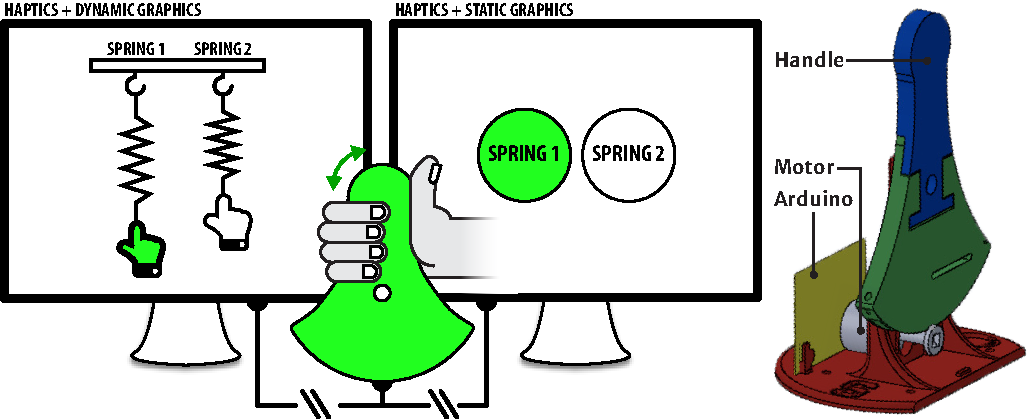
\includegraphics[width=0.7\textwidth]{handson/cyberhap-interface_pb}
  \caption{In the \textit{Hapkit+Dynamic Graphics} condition, graphical springs responded to input (left); static images were rendered in the \textit{Hapkit+Static Graphics} condition (right); in both, HapKit 3.0\cite{Martinez2016} was used as an input/force-feedback device (far right).}
  \label{fig:study1-hapkit}
\end{figure}

\subsubsection{Discussion:}
Study 1 revealed that (a) for stiffness intervals 15/35/55/75 N/m, the HapKit  provides  distinguishability equivalent to  dynamic graphics.
%, lending promise to the hapkit’s use even without visual reinforcement. 
Individual differences influenced difficulty and speed, 
%adding to the literature on individual differences for haptic perception and 
 suggesting that learning interfaces may need to accommodate this variability. % in user responses. 
(b) Accuracy was not dependent on individual differences, suggesting that learning interfaces can consider task time and perceived difficulty separately from accuracy when using the HapKit (at least, for these force ranges).
%We also found 
(c) Performance was mostly above 90\%, and confidence intervals for our small sample size estimate no lower than 82\% accuracy at the lowest (15/35). 
%Although the low value for spring pair 1 was initially unexpected (Weber’s law (cite?) predicts that spring pairs 2 and 3 should be more difficult because of a lower proportional difference), 
We speculate that the HapKit's natural dynamics are more pronounced at lower rendered forces, and may interfere with perceptibility. 
%This is a targeted area for future improvement.
%
\subsection{Study 2: Tool Usability and Educational Insights}

%
\subsubsection{Methods:}
%\paragraph{Participants}
10 non-STEM participants (1st and 2nd year university undergrads with up to first year  physics training, 6 female, 17-20 years) volunteered for 45-60 minute sessions.
%\paragraph{Protocol}
After an introductory survey, participants were randomly assigned to one of two conditions, \textit{Mouse} (4 participants, M1-4) or \textit{Hapkit} (H1-6).
%The assigned condition determined the input device used to manipulate virtual springs in SpringSim.
HapKit 3.0 was calibrated for force consistency between participants.
After allowing participants to freely explore \SpringSim, % for several minutes, 
a survey assessed % participant's 
understanding and usability of various \SpringSim interface components;
misunderstood components were clarified.
%The facilitator conducted a debrief following the survey to avoid the interference of usability issues while assessing learning strategies and use cases of HapKit 3.0 during the education tasks.
%Participants then worked through 7 education-based tasks on springs and spring properties,
%each followed by a brief interview. 
Three exit surveys elicited 
value of \SpringSim components on 7-point Likert scales, 
cognitive load~\cite{jones_1990}, understanding, and curiosity on 20-point scales,
and preferred learning modality~\cite{vark}, respectively.

%Interview followed each task; after the last task, three exit surveys were conducted:
%one evaluating value of \SpringSim components,
%one cognitive load \cite{jones_1990},
%the last preferred learning modality \cite{vark}
%the first of which assessed the value of \HandsOn components. This assessment of conceptual components, as opposed to interface components, was possible due to the usability debrief that reasonably removed the interface implementation as a confound to the value of \HandsOn components. The following exit surveys assessed cognitive load \cite{jones_1990} and preferred learning modality (CITE VARK), respectively
%A closing, semi-structured interview fielded information on HapKit 3.0, SpringSim, and participant insights during the
%Sessions lasted 45-60 minute session.

\subsubsection{Learning Tasks:}
We iteratively designed and piloted a task battery of escalating learning-goal sophistication~\cite{bloom1969taxonomy} to
 %; when carried out, they must
expose strategies for force feedback use and general problem-solving (Table~\ref{tab:SpringTasks}).
Tasks did not require physics knowledge,
 % more generally.
% As with \SpringSim, they
and were suitable for both mouse and HapKit input.
%as input device, without overtly favoring either one.
%Participants in Study 2 were asked to sequentially carry out the tasks in .

%\todo{OS: how do you use both 'c' and 'p' in tabular?}
% https://en.wikibooks.org/wiki/LaTeX/Tables
%\osC{slc}
%02.07 OS: I don't think you can use c and p. You can achieve finer control by using multirows and multicolumns, but it gets trick.
\begin{table}[tb] \footnotesize
    \begin{tabular}{|p{0.40in}|p{1.00in}|p{3.3in}|}
    \hline
    \textbf{Task} & \textbf{Bloom} &  \textbf{Description} \\ \hline
    1    & Understand (2) &  Rank three springs in order from least to most stiff  \\ \hline
    2    & Understand (2) & Plot the relationship between displacement and force for two springs. \\    \hline
    3    & Apply (3) & Estimate the stiffness of an unknown spring, given two reference springs with known stiffness value \\ \hline
    4    & Analyze (4) & Predict the behaviour of springs in parallel. \\ \hline
    5    & Create (6) & Design a parallel spring system that uses two springs to behave like an individual spring of stiffness 55 N/m. \\ \hline
    6    & Apply (3)  & Predict the behaviour of springs in series. \\ \hline
    7    & Evaluate (5) & Describe any relationships you have noticed between spring force, displacement, and stiffness. \\ \hline
    \end{tabular}
    
    
    \caption{Learning tasks used with \SpringSim in Study 2. \textit{Bloom} level is a measure of learning goal sophistication \cite{bloom1969taxonomy} %, \textit{Input} = anticipated input device, Mouse/HapKit.
%        \caption{Learning tasks used with \SpringSim in Study 2. Diff $=$ relative difficulty, Input = anticipated input device, M = mouse, H = hapkit.}
%    \kmC{Impt: Table needs to list ''Bloom level (a measure of task sophistication [CITE]'')} 
 %   \gmC{Karon, can do, but do we feel it is important, valuable enough to replace the current difficulty column? Explaining blooms will take some space...}
   % \kmC{(1) I believe Bloom is better to list. I hope this description in caption is sufficient.}  
   % \kmC{(2) want to drop  input type?} (was impt at one point) 
   }
   % GM: yes, dropping input. was impt when we were considering adding tasks that favored one condition over another. we never did move forward with that. 
   
    \label{tab:SpringTasks}
\end{table}

%
\subsubsection{Analysis:}
%Through both quantitative and qualitative analyses, common themes have been identified.
We conducted t-tests on self-reported understanding, cognitive load, engagement, understanding, curiosity; and on objective metrics of time-on-task and number of spring interactions.
Qualitative analysis of video and interview data used grounded theory methods of memoing and open \& closed coding \cite{Corbin2008}.
Together, these  yielded insight into the usability of \SpringSim and the \HandsOn CM, and several themes %(reflecting the \HandsOn conceptual model).several themes
describing the role of haptics in our tasks. Two participants were excluded from analysis of Task 1 due to technical failure. %\osC{GM, put reason in comments please} \gmC{slc}
% GM: The participant either misunderstood, or I forgot to instruct them to turn the 'stiffness display' off, which spoiled the question.
%OS: Thanks. Leaving here for posterity.


%\kmC{Some left out of analysis??} % later you reference 'participants included in analysis'.
%, observations about our tasks,

%First we present the major findings that provide initial insight into the use of a haptic-enabled interface for education tasks. Later, we outline the effectiveness of the educational task set and present usability results of \SpringSim and its conceptual model \HandsOn. 

 %Paired t-tests were performed to analyze changes in participants' self-reported understanding throughout educational tasks. Two-sample t-tests were performed to determine effects of condition (Hapkit or Mouse) on self-reported cognitive load metrics, engagement, understanding, curiosity, time spent exploring, and spring interactions. Qualitative methods included analyzing screen recordings, video data, and interviews using grounded theory methods; primarily memoing, open, and closed coding techniques (CITE). \gmC{OS, we should perhaps have brief discussion to ensure this is being described appropriately.} 
 
 
\subsubsection{Results - Usability:}
%\paragraph{\SpringSim \& \HandsOn provided robust learning environment}
%\SpringSim and its conceptual counterpart \HandsOn provided a platform on which students were able to successfully attempt all presented tasks in both HapKit and Mouse conditions with few. 
%
%Following the completion of free, exploratory interaction with \SpringSim, participants were asked to indicate wether or not they understood the intended functionality of each
%\kmC{?? SLC} % what is the 100\%? are these # of respondents, binary response? clarify. Consider reporting out of x/n instead of %.}

After free exploration of \SpringSim, participants rated their understanding of CM objects (yes/no) and their ease-of-use [1-7]:
\emph{Ruler} (10/10, 7.0),
\emph{Numerical Force Display} (10/10, 6.5),
\emph{Playground} (10/10, 6.0), 
\emph{Hand} (9/10, 6.0),
\emph{Spring Properties} (9/10, 6.0), 
\emph{Spring Generator} (\textbf{\textbf{7/10}, 5.0}),  
\emph{HapKit} (6/6, \textbf{4.5}), and
\emph{Haptic Feedback Controls} (5/6, \textbf{4.5}). 
%
While generally usability was good, interface clarity needed improvement in highlighted cases. 
Participants specifically noted confusion on radio button affordances, %color scheme of %\kmC{??} 
%ControlP5 radio buttons, where lighter shades of red counter-intuitively indicated an active selection
and \emph{Spring Generator} input fields (due to redundant availability in \emph{Spring properties}).

%After free exploration of \SpringSim, \kmE{most??} participants reported understanding most CM objects:
% % \SpringSim components: 
%\emph{ Force Display} (100\%), \emph{Playground} (100\%), \emph{Ruler} (100\%), \emph{HapKit} (100\%), \emph{Spring Properties} (90\%), and \emph{Hand} (88\%).
%% Less understood were
%\kmE{More had difficulty with} \emph{Haptic Feedback Controls} (83\%) and \emph{Spring Generator} (70\%).
%% Participants rated 
%Ease-of-use ratings [1-7] yielded median scores $>=6$ % or higher 
%% for Force Display (6.5), Playground (6.0), Ruler, (7.0), Hapkit (7.0), Spring Properties (6.0), and Hand (6.0).
%Median scores were lower for the Spring Generator (5.0) and HapKit Feedback (4.5).
%Participants noted confusion on color scheme of ControlP5 radio buttons and input fields in the `spring generator' (also available in the `spring properties' component).

%who made it unclear to some which selection was currently active. Sentiments such as "I'm not getting the colors" (H1) were commonly expressed.
%Furthermore, some participants displayed confusion about what the text input fields in the `spring generator' would affect. 
%This was likely due to having presented spring properties in two places: both in the ‘spring generator’ and ‘spring properties’. Future iterations should provide a better mapping of spring properties to existing springs, and settings in the spring generator to springs being designed. 

%Once all visual and haptic feedback displays were enabled, no participants were observed manipulating either Numerical Forces or Hapkit Feedback.
%attempting to turn off hapkit or numerical feedback displays, nor adjusting the gain of the hapkit device. 
%Occasionally, participants would attempt an unpredicted exploratory behaviour that was not supported by \SpringSim. M2
%, in his initial exploration of the system,
%attempted to design a spring with K=10000 N/m.
%In its current implementation, the software was capable of handling this value, however, the hapkit was not. \osC{not really sure what do about this factoid} \gmC{I added clarification, try now} \kmC{SpringSim did support it - don't say it didn't. SpringSim is not HapKit.}
%type of exploration, however, what should  a K-constant of 10000 N/m feel like on the hapkit? To render such a force is unrealistic, and without limits in place, there is risk of damaging the HapKit hardware, or providing inaccurate feedback.

\subsubsection{Results - Task Suitability for Haptic Research:}

%\kmC{Is this section about task suitability? SLC}. % Suitability for what? In any case it's not about what they learned, which is what heading seems to suggest. but I'm not sure it will support a conclusion about suitability. Data describes that they're possible to do, and likely balanced between mouse/hapkit input. does not reveal engagement, too easy, relation to learning goals etc.

Regardless of prior physics knowledge, all participants were able to complete education tasks 1-6 (Table \ref{tab:SpringTasks}) in the allotted 60 minutes. 
%Further, all participants were able to attempt the tasks, regardless of their prior physics knowledge. 
%Tasks intended to support multiple workflows (1,3) did so, and participants found an answer irrespective of condition. 
%\kmC{?? SLC} % clarify. you say additional workflows were OBSERVED (not designed?) then imply 'other than these observations, none were DESIGNED.
We found no evidence that any task favoured %Besides additional workflows having been observed in the HapKit condition, no tasks was designed to favor
one condition over another.
When participants in the mouse condition were asked how their workflow would change %have changed
with physical springs, participants weren't sure: ``I don't know if that would've given me more information" (M4). 
%``... I don't think that would make a difference... But, 
%you know,
%the last question, 
%if it was two springs [in series], it would be easier to answer that question." (M3).
%However, no participants in either condition had access to a serial spring system \gmE{to answer the question referenced by M3, which was intended to be elicit predictions.}% \kmC{Why relevant?} \gmC{try now}
 
\subsubsection{Results - Haptics \& Learning Strategies:}
We observed several themes relating to the influence of force feedback % haptics 
on a student's learning strategy. %, elaborated below.

%(1) Forces increased a participant's possible strategies, and \kmE{sometimes ?}created} \kmC{?? predominating?} new strategies.  % KM - I don't understand "created predominating new strategies".
%(2) Haptic interactions with springs were impressionable and persuasive. 
%(3) Participants in the haptics condition reported increases in curiosity & understanding throughout the lesson. 
%(4) The issue of perceptual resolution in haptic devices for education.

%\paragraph{Haptics changes and provides additional workflows}
\paragraph{Haptics creates new, dominating strategies.} %\kmC{?? FIX, SLC} % i don't understand this sentence at all, nor 'predominating new strategies' in earlier statement. Not english.
%
Learning strategies used by participants %were employed between participants
in the HapKit condition (H1-6) were more diverse than those in the mouse condition (M1-4).
In Task 1, M1-4 all followed the same strategy, displacing all 3 springs the same distance and comparing the numerical force required to displace them. They then correctly inferred that higher forces are associated with stiffer springs (the \textit{displace-and-compare} strategy).

By contrast, all 5 H participants included in analyses (H2 excluded due to technical failure) used force-feedback as part of their  approach to Task 1. 
H1 describes applying the same force to the HapKit across all 3 springs, recording displacement to solve the task, while
H5 described looking at the speed at which the HapKit was able to move back-and-forth in making his determination of stiffness, rather than through direct force-feedback of the device. Only H6 indicated that he ``looked at the numbers for a sec", but no participant fully used the \textit{displace-and-compare} strategy we observed for M participants. 

%OS 02.08 make sure KM's comment below is handled in discussion.
%\kmC{The single M strategy worked well. Why is diversity a benefit?}
While the single-strategy approach worked for easy tasks, it was linked to errors and dead-ends in at least one instance in the mouse condition.
In Task 5, M2-4 used  \textit{displace-and-compare}  to validate their newly designed spring; M1 did not seek verification of his design.
In contrast, H1,2,5,6 used haptic feedback to verify their designs. % of a parallel spring system.
They did this by comparing how stiff their parallel spring system felt to a target reference spring. 
H4 guessed at an answer without verification.
H3 used the \textit{displace-and-compare} strategy, checking that equal forces were required for equal displacement. %of each spring.


% GM IS REMOVING THIS AT HIS DISCRETION 02.08:

%\paragraph{Haptics allows students to test, revise hypotheses similarly to status-quo methods.}
%\osC{Do we want to say ``similarly to status-quo methods" in the results?}
%\osC{This section should go before "diverse workflows} \gmC{I'm not sure how valuable this is... RD, any opinions on keeping section:}
%We found participants in both conditions followed a very similar hypothesis-testing process for Task 5, beginning with a hypothesis of what the spring system's components should be, implementing it, and reading feedback using the numerical force display in the mouse condition (3/4) or used either numerical force display or force-feedback in the hapkit condition (5/6). In each condition, there was one participant who developed a hypothesis, implemented it, and did not seek to verify their result. 
%No significant differences were found between the number of iterations that participants performed for their design of a parallel spring system between HapKit and mouse conditions in Task 5. 

%\paragraph{Haptic interactions with springs are impressionable.}
\paragraph{Haptic impressions of springs are enduring and transferrable.}
%\kmC{Impressionable?? or 'haptic impressions of springs are enduring and transferrable'.}
HapKit participants were able to use their previous explorations to solve problems.
In Task 3, M1-4 interacted with all three springs to find a ratio between force and stiffness.
However, H participants interacted with springs fewer times (mean 1.5, sd 3.21) than M (6, sd 1) (p=0.018). %(t(6.5161)=3.1429; p=0.0179).
H2-4,6 did not interact with any springs,
%during the task,
and H1 interacted with only one.
This was because they had already 
%Participants in the hapkit condition who did not interact with springs cited having already
interacted with the springs in previous questions: 
%``it was just kind of intuitive" (H2);
``I remember spring C was less stiff" (H3).
%H1: "I used what I did for the first one... I knew it was pretty not stiff [sic]",.
 Further suggesting the strength of haptic impressions, % impressionability of haptics,
 %is futher highlighted by
 when H1 designed an inaccurate spring system for Task 5 (k=80N/m vs. expected k=55N/m), 
 she described the haptics as overriding the visual feedback: %``when I felt it, they just felt similar.
 ``they just felt similar.
 Even though the numbers weren't really relating to what I thought."
 Similarly, H2 arrived at an approximate result (k=40N/m), after using force-feedback and acknowledges ``... [it's] slightly less than the reference spring, but it's closer."
  %but seems to %acknowledge andignore the fact it remains inaccurate:
 %inaccurate but still a final answer: . \osC{could cut this last example if need be}
 %She appeared  to use both the force-feedback from the hapkit, in addition to the strategy of using numerical force feedback commonly seen in the mouse condition: “
 when I felt it, they just felt similar. Even though the numbers weren’t really relating to what I thought.”

%GM: I do feel that there is something here, but we're really starting to tread on grounds of educational utility, which I think we should steer clear from.
%\paragraph{Using haptics led to more approximate answers}
%A common pattern observed in the hapkit condition is a tendency for participants to arrive at at answers that they cite as being approximate. H4, Task 2: "the numbers are just kind of random", P9, Task 5 "they kind of matched"; H2, Task 5: "its slightly less than the reference spring, but its closer", H6, Task 5: "I can't really confirm its correct, but they both feel about the same". In task 3, participants in the mouse condition were seen interacting with springs in a productive manner as they worked towards a calculation. This was not observed in the hapkit condition, as previously mentioned. For task 5, 3/6 participants in the hapkit condition arose at answers that were not accurate. This is compared to 3/3 in the mouse condition who all provided accurate answers. 

\paragraph{Haptics associated with increases in self-reported curiosity and understanding.}
%\kmC{earlier said 7-point scale?? clarify earlier}
Participants' self-reported curiosity significantly increased over the course of HapKit sessions 
from a mean of 6.3 (sd 3.83) %median, sd, min, max =  5/ 3.83/ 2 /12)
to 10.8 (sd 3.92) in the Hapkit condition %t(5)=-2.7302; 
(p=0.041). %0.04127.
No significant changes in curiosity were detected in the mouse condition.
Participants' self-reported understanding significantly increased over the course of HapKit sessions from a mean of 3.67 (sd 4.03) to 11.83 (sd 3.19) (p=0.014). %(t(5)=-3.6914, p=0.0142).
No significant changes in understanding were detected in the mouse condition (before: 9.25, sd 5.32; after: 9.25, sd 5.32; p=0.77). % t(3)=0.31363; p=0.7743).
%We acknowledge the discrepancy between conditions in participants' self-reported understanding at the beginning of the session. \todo{include more in discussion} \osC{Is this last sentence worth mentioning? Do we already have it in discussion? I recommend cutting}

In interviews, participants commonly made references to how the HapKit influenced their understanding: ``I can use this thing for help if I really need some physical, real-world stimuli" (H5); % to help me solve questions on the sheet" (H5);  %``the question about parallel springs and regular springs and the stiffness, 
%``[when] we looked at it mathematically I could find the answer if I was given a formula, but I think just having the hapkit and just physically testing it out was really, really helpful"% and made it very clear what the answer should be”
%(H2).
``almost all of my thinking was based on how the spring [HapKit] ended up reacting to it" (H6).
%\osC{another quote in comment; not sure which is better}
%``Like, I wouldn't have figured out one of those tasks if I didn't have the spring [HapKit)]to test out if these two were similar or not" (H6).
M2, who had a stronger physics background than others (IB Physics),  was the only user to report a drop in curiosity and understanding over the course of the physics tasks, despite initial excitement:
%At first, M2 expresses his excitement and curiosity of the interface, which was presented in the mouse-only condition:
``the fun part is messing around with  [SpringSim]," he exclaimed near the beginning of the exploratory phase. 
%Throughout the lesson, he demonstrates a level of understanding about springs that was above other participants, and ponders several questions relating to the frequency of spring motion, the effect of angles on springs in parallel systems, and others [include concrete example] that SpringSim was never intended to support.

%\paragraph{The issue of perceptual resolution seen in HapKit.}

%\gmC{GM acknowledges a missing section presenting critical incidents of two separate participants that were 'misled' by the haptics due to its perceptual quality. Will insert data in am of 02.08. This data must have been inadvertantly cut in an edit}    


%
\subsection{Study 2 Discussion} 
%
% We discuss implications for design and implementation of haptics for e-learning tasks, including limitations and direction for future work. 
%
%Discussion:
%    - Hapkit 3.0 -> perhaps for exploration over accuracy. 
%        - discuss its impressionability, how that at times it appeared to suppress alternate workflows that would lead to a more accurate results than by feel alone.  
%        - present it as a design challenge: students still have access to the tools and workflows that would help them arrive at a correct answer, but it currently seems to be suppressed. 

%    -Why approximate answers -> impressionability and resolution of the hapkit together, create a situation where students are empowered to use haptics in their problem-solving, but are limited to the accuracy and resolution of their solution. This could have design considerations, and 
    
%    - Design consideration: "zooming in on haptics" -> solve limits on perceptual ability through recommending haptic "gain" or "zooming in on haptics".

% ----------------------
\subsubsection{Tool and Tasks: Suitability for Learning and as Study Platform}
% -----
\paragraph{Adequacy and comprehensibility of underlying model:} Overall,  \HandsOn  concepts proved an effective and comprehensible skeleton for \SpringSim. 
% Concepts that shone through the interface were well received by participants. 
Specific implementations rather than concepts themselves 
 % There were no concepts, but rather specific implementations, that 
 appeared to be the source of the reported confusions, and 
 we observed that \HandsOn should be extended % needs to be modified slightly  to support the future incorporation of 
 with additional measurement tools (e.g., protractors, scales, calculators, etc). 
 % Here we briefly discuss the performance and limitations of \SpringSim.

% -----
\paragraph{\SpringSim performance:} %performance and limitations:} 
This \SpringSim implementation adequately supported most students in finishing learning tasks; 
extending available objects, properties and tasks will support advanced students as well.
Future iterations should 
%
% resolve some concerns from participants; including 
more clearly map \textit{Design Palette} elements to the objects they support, 
% Spring Properties to the Springs, moving 
increasing rendering fidelity and reconsider colors to avoid straightforward affordance issues.
% (eg, participants were confused by the color scheme of the radio buttons). 
While participants did not heavily use haptic and visual controls, we anticipate these will be important  for instructor and researcher use. 

% -----
\paragraph{Learning task suitability:}
The learning tasks used here were fairly robust to time constraints of user-study conditions, did not require previous physics knowledge, avoided bias % contamination 
from standardized physics lessons, and exposed haptics utilization strategies without penalizing non-haptic controls. 
Currently, the task set ends 
% with a cliff-hanger for participants, 
by asking students to predict a serial system's behavior; some students found predicting new configurations a large jump.  % Gordon: is this because it was intrinsicly harder than parallel systems, or because they couldn't try it out?
% \gmC{because its an instrically harder problem. It was a prediction question, so wasn't made more difficult by not being able to try it out - although that would've helped, too}
%\kmC{GM: Does below capture?}
% This seemed to be a much more difficult and less-intuitive problem for participants to think so, 
% It would be beneficial for future iterations if
Future task-set iterations could support integrative, prediction-type questions with interface elements that are successively exposed to allow prediction testing.
% Am picturing a system that only lets them try out serial assemblies after they've thought about it and mcommitted to a guess. 

% such leaps with an interface implementation to allow them to explore behavior.
% should support more object-connection possibilities, to gather  such functionality to elicit further information about the use of haptics over an even greater range of task difficulty. 


% ----------------------
\subsubsection{Evidence of the Role of Force Feedback in Learning}

% -----
\paragraph{Curiosity and understanding leading to exploration:}
Self-reported curiosity and understanding increased when forces were present. 
%GM: In mouse condition, no significant increase was found for curiosity. However, participants in mouse condition started with a much higher self-reported curiosity than in hapkit condition. so we can't conclude that haptics increased curiosity while mouse did not... 
 %KM: This is a statistical anomaly right? at start, an unbiased sample should have given same response to self-reported curiosity, or did the condition have a chance to influence this?
%GM: Yes, a random number generator assigned conditions - statistical anomaly (... and exact same protocol in both conditions leading up to their responding to initial curiosity question)  
%
%
% Due to the informal and self-reported nature of evaluating participant understanding, we leave any indication of significance to future research. 
While these trends must be verified, curiosity is of interest since it can lead to more meaningful and self-driven interactions.
% the observed increases in curiosity is an interesting finding with implications of its own. 
%
Iterations on both tasks and tool should support this urge with an interface and framing that supports curiosity-driven exploration.

% -----
\paragraph{Alternative strategies enabled by force feedback:}
%
The HapKit's additional feedback modality enabled alternative task workflows, e.g., %by providing another modality with which to receive feedback. 
% (Table \ref{tab:SpringTasks}), 
 estimations of force appeared to supplant mathematical strategies for stiffness estimation.
% Perceived forces dominated several participants' strategies, % and seemed to provide non-specific feedback in participants' hypothesis testing. 
While possibly risky as a crutch, force assessments might be a useful step for students not ready for technical approaches (e.g., M3/Task 3 when  stalled in attempting cross-multiplication).
Future task-set iterations could encourage more \textit{balanced} strategy use, e.g. mathematical \textit{and} perceptual rather than primarily perceptual.

%\kmC{GM: this might not be a BETTER strategy. comment? ``Future task-set iterations could more strongly encourage equal use of multiple strategies, e.g. mathematical \textit{and} perceptual rather than primarily just perceptual.}



% -----
\paragraph{HapKit salience, resolution \& implications:}
Overall, HapKit 3.0's fidelity was enough to assist participants verify a correct hypothesis. 
% It could point a \textit{direction} to revise one that proved to be incorrect, but 
% While the feedback was helpful in guiding students towards a more accurate hypothesis, 
%its rendering resolution and accuracy did not suffice to lead them all the way to an accurate result. Overall, 
However, those who started with an \textit{incorrect} hypothesis and used only HapKit to test it generally arrived at solutions that improved but were still inaccurate. 
Given the confidence that forces instilled, % impressionability of haptics that was observed, 
this is an important consideration.
%
 A formal device characterization will allow us to keep tasks within viable limits; 
 % to inform future design; 
  we can also consider using low-fidelity forces more for reinforcement and exploratory scenarios. % or encouraging its use in accompaniment with other strategies.
 % to avoid scenarios previously described (H1), in which a student over-rules her observation of what visual feedback is telling her, in favor of haptic feedback, which proves inaccurate.

 
% -----
%\paragraph{Is tool ready for a learning study?}

% - Explain the kind of study it is currently suitable for (or not suitable for).
 
% - two parts: (a) good so far (right direction); 
% (b) does it need to be extended, more complex/engaging?


% ----------------------
\subsubsection{Limitations and Next Steps:}

% -----
% \paragraph{Limitations:}
Our studies were small and used non-STEM university students as a proxy for high-school learners.
Despite both limitations, they were useful for our current needs (rich, initial feedback establishing suitability and usability for \HandsOn through \SpringSim);  % but suggest future elaboration with larger, more targeted participants.
%We feel this proxy sufficed for physics knowledge but
but may overestimate general academic ability and maturity.
%. This compromise served our purpose insofar as
%eliciting feedback on tool suitability and haptics-enabled exploration strategies; a test that \SpringSim has largely passed.
As we we move into evaluation of learning outcome impact, larger and more targeted studies are imperative.

% but as we we move into evaluation of learning outcome impact, larger and more targeted studies will be imperative.}
 
% -----
% \paragraph{Future Use and Development:}

 % This study largely validates \SpringSim for learning outcome assessment contains the components and task set that would support more comprehensive educational studies that should be carried out.
%Beyond details noted above, 
Future interfaces can both increase physical model complexity and breadth (e.g., complex mass-spring-damper systems), and extend \HandsOn for more abstract education topics, such as trigonometry. 
 We also plan to extend the \textit{Playground} to support more engaging, open-ended student design challenges, such as obstacle courses using trigonometry concepts; this in turn requires new measurement tools and tasks that are more exploratory and open-ended.
 % such as a protractors and grid rulers. A c
% Accompanying challenge tasks must encompass exploratory and open-ended styles.
 % and follow the requirements of the current task set to further support the study of haptic-enabled educational interfaces.
 
 %Iterations of \SpringSim and its task set should implement the aforementioned usability modifications, include support for serial spring systems for a greater range of task difficulty, take into greater consideration the perceptual qualities of the HapKit, and better account for a student's desire to explore beyond the renderable range of haptic feedback devices. 

% -----
%\paragraph{Planned Interface Evolution} 
%- future complexity; talk about how our CM can handle a very different interface (design playground to build, for example, obstacle courses, contests between friends, etc. New measurement and assessment tools.





% -----
%KM: \paragraph{Middleware to support flexible, dynamic haptic models} Very briefly allude %to need for new programming support for reconfigurable handles. No detail.
%GM: moved to FW for now, until I find a relevant place in discussion





% =========================================
\subsection{Conclusions}
%

% We have presented initial insights into the influence of haptics in e-learning tasks. 
Haptic feedback's potential in STEM education use can only be accessed with a comprehensible, extendable, and transparent front-end. 
We present \HandsOn, a conceptual skeleton for interfaces incorporating virtual forces into learning tasks,
%to access the posited benefits of tangibility with the accessibility, power and flexibility of virtual environments.
and assess its first implementation, \SpringSim and task set. 
Our findings (on interface usability, task effectiveness, and impact of haptic feedback on learning strategies, understanding and curiosity) underscore this approach's promise, as we proceed to study haptic influence on learning outcomes themselves.




\section{CuddleBit Design Tools: Sketching and Refining Affective Robot Behaviours}
\label{sec:applications:cuddlebit}
In \autoref{sec:applications:cuddlebit}, we explore a third non-vibrotactile modality - furry, affective, breathing robots called CuddleBits (\autoref{fig:cuddlebits}).
These robots are multimodal: they visibly move, and their breathing can be felt.
Their form factor and affordances can vary; for example, they can be flexible (\autoref{fig:flexibit}) or rigid (\autoref{fig:ribbit}).
We use the CuddleBits as a rich design problem - supporting engaging, emotional, lifelike behaviour design - and as a means to explore the interplay between two design tools, each supporting different activities: \emph{sketching} and \emph{refining}.

As robots begin to take a larger role in our lives, they require natural ways of interacting with people.
Notably, they need to communicate affectively with humans, recognizing and expressing emotion, or behaving with a \osE{believable} personality.
This is important for both everyday interactions with robots, and targeted health applications: robot-based therapy can measurably relax people by breathing \cite{Sefidgar2016}.



\begin{figure}[htbp] %  figure placement: here, top, bottom, or page
   \centering
      \begin{subfigure}{0.5\textwidth}
   	   \includegraphics[height=1.6in]{cuddlebit/flexibit} 
	      \caption{``FlexiBit", a furry, flexible CuddleBit.}
	      \label{fig:flexibit}
   \end{subfigure}
   \qquad
   \begin{subfigure}{0.4\textwidth}
   	   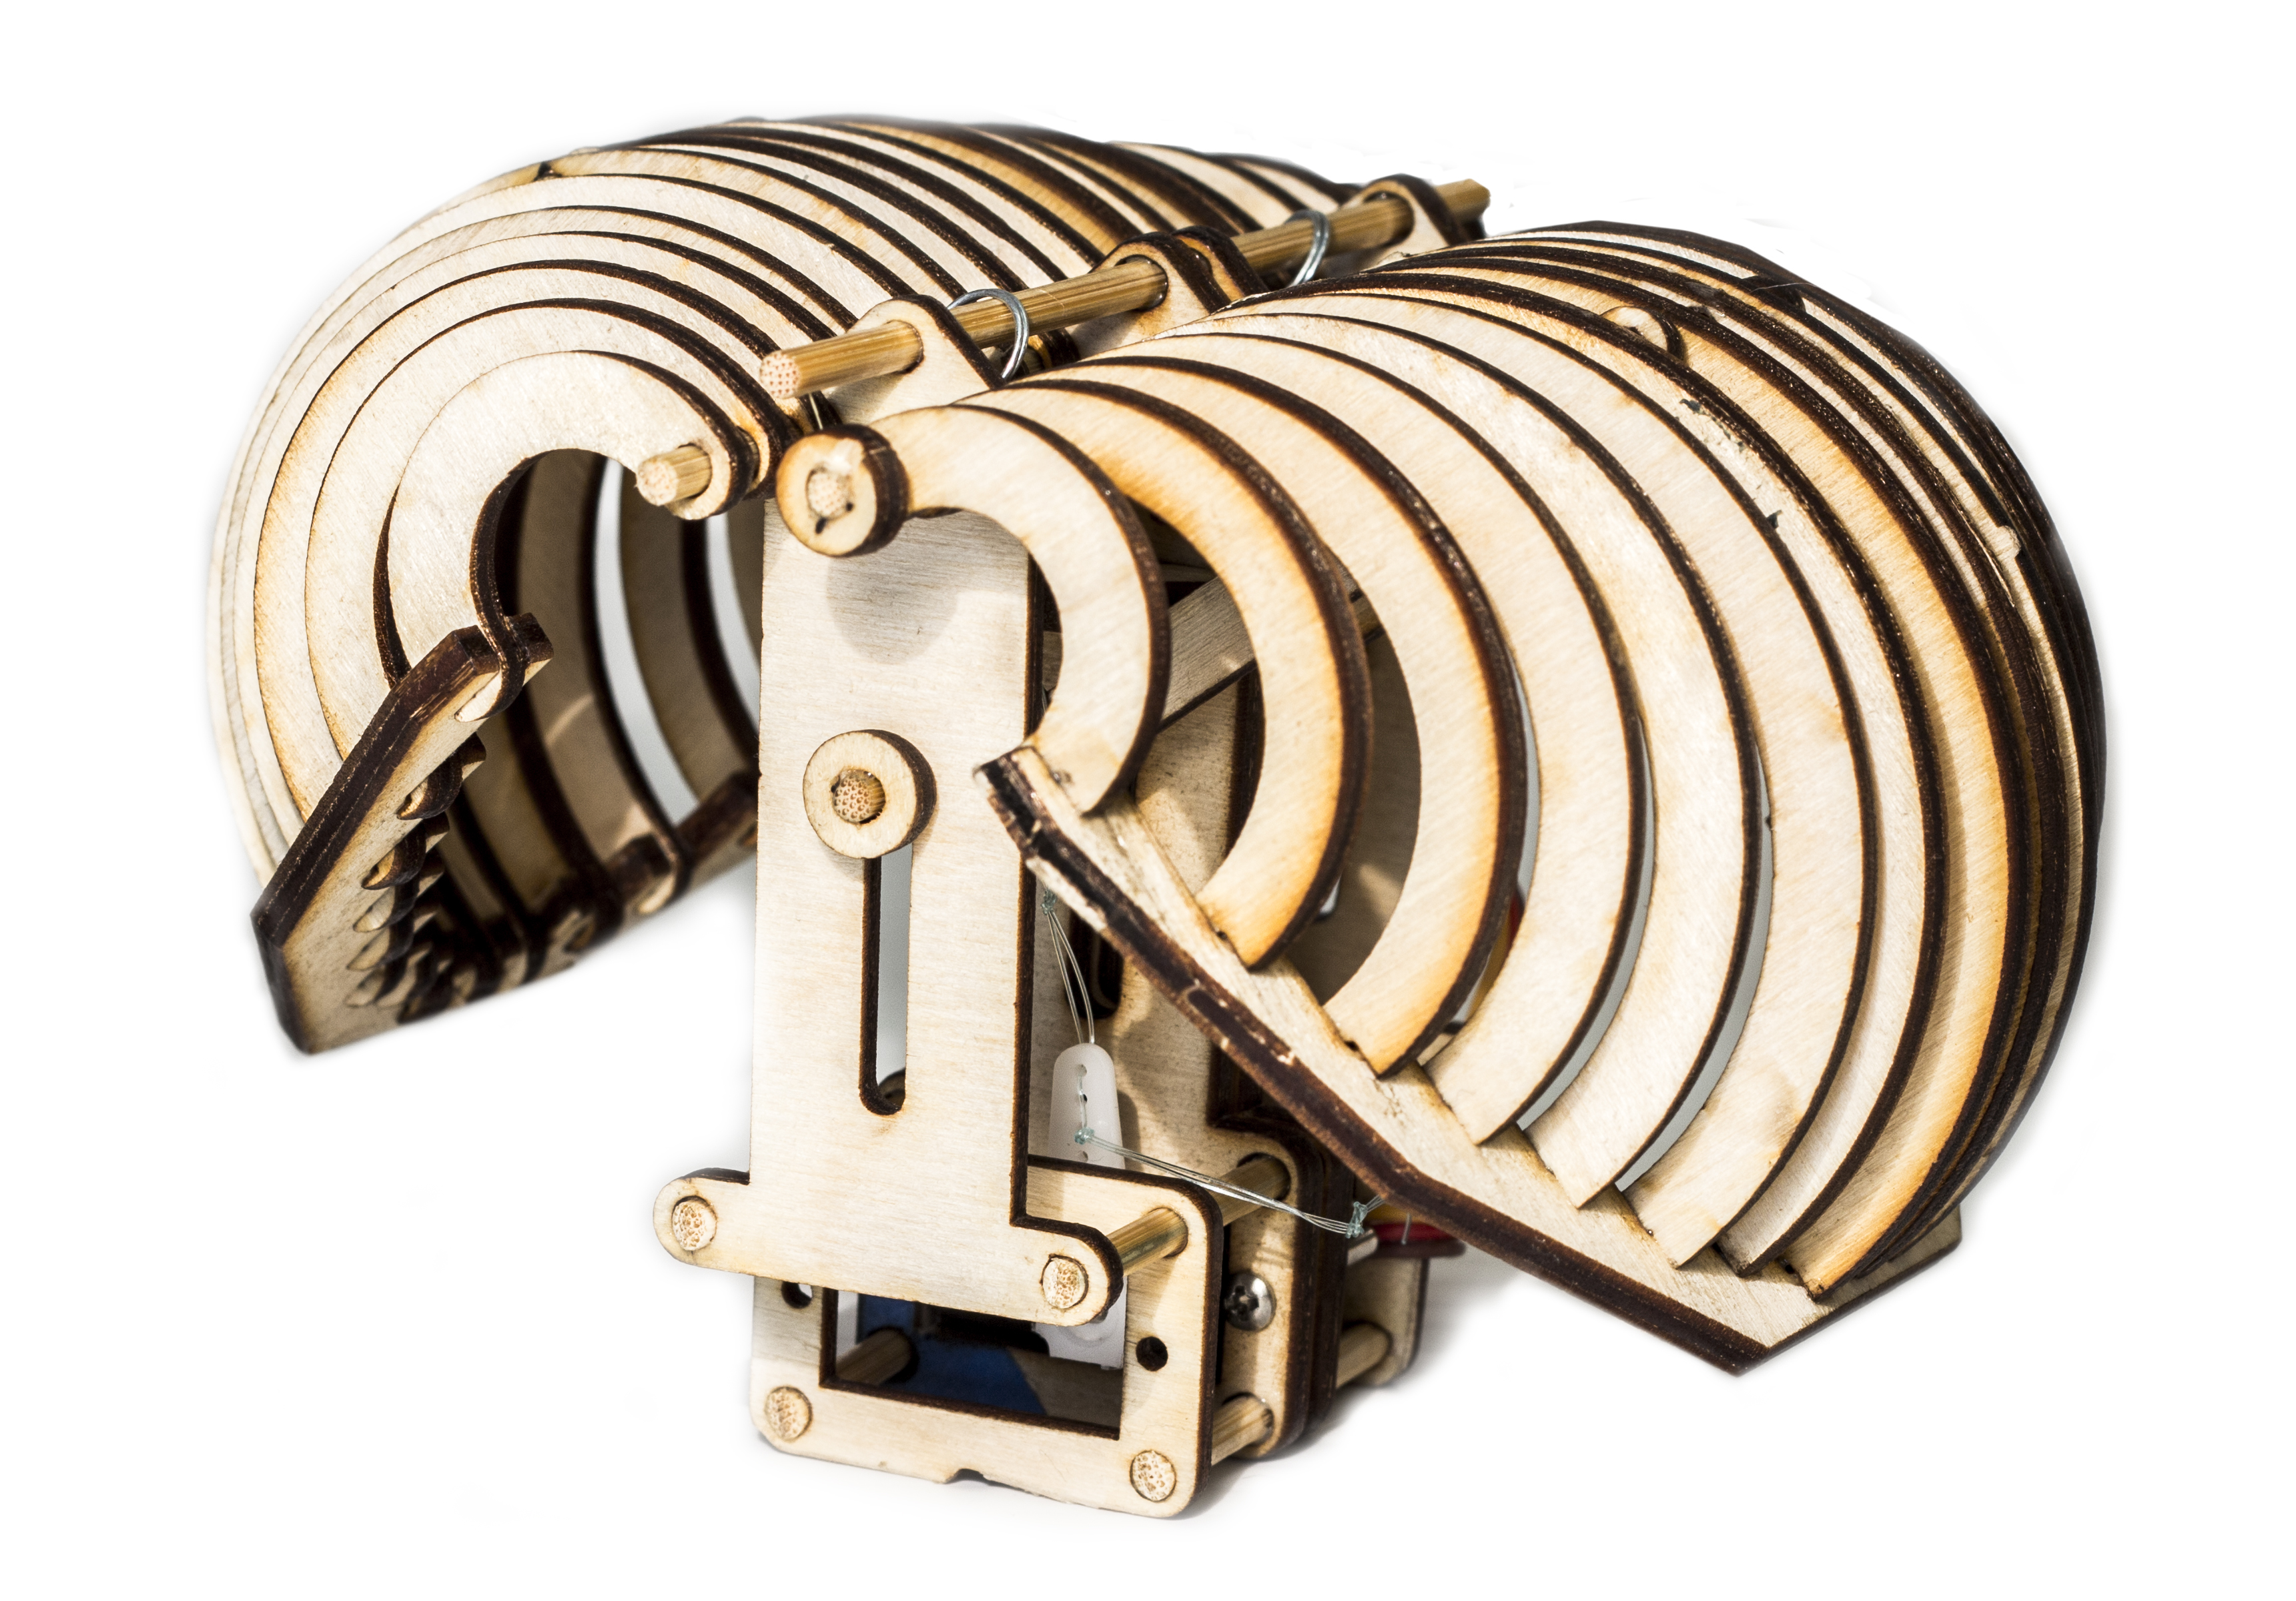
\includegraphics[height=1.6in]{cuddlebit/ribbit-open} 
	      \caption{``RibBit", a rigid CuddleBit.}
	      \label{fig:ribbit}
   \end{subfigure}
   \caption{Two examples of CuddleBits, simple DIY haptic robots.}
   \label{fig:cuddlebits}
\end{figure}



The Haptic Creature project \cite{Yohanan2011affectdisplay,Yohanan2011affectivetouch} explores the role of touch-based interactions with furry, zoomorphic robots.
However, an early prototype of a multi-DoF haptic robot, the CuddleBit, suffers from slow iteration for both hardware form-factor and software behaviours.
To explore these concepts more thoroughly, we developed the CuddleBits \cite{cang2015cuddlebits}: simple, affective robot pals built with a rapid prototyping (sketching) ethic.
To control CuddleBit behaviour and inform \haxd support tools in this complex domain, we developed two software design tools: Voodle and MacaronBit (\autoref{fig:cuddlebitdesigntools}).

\begin{figure}[htbp] %  figure placement: here, top, bottom, or page
   \centering
      \begin{subfigure}{\textwidth}
   	   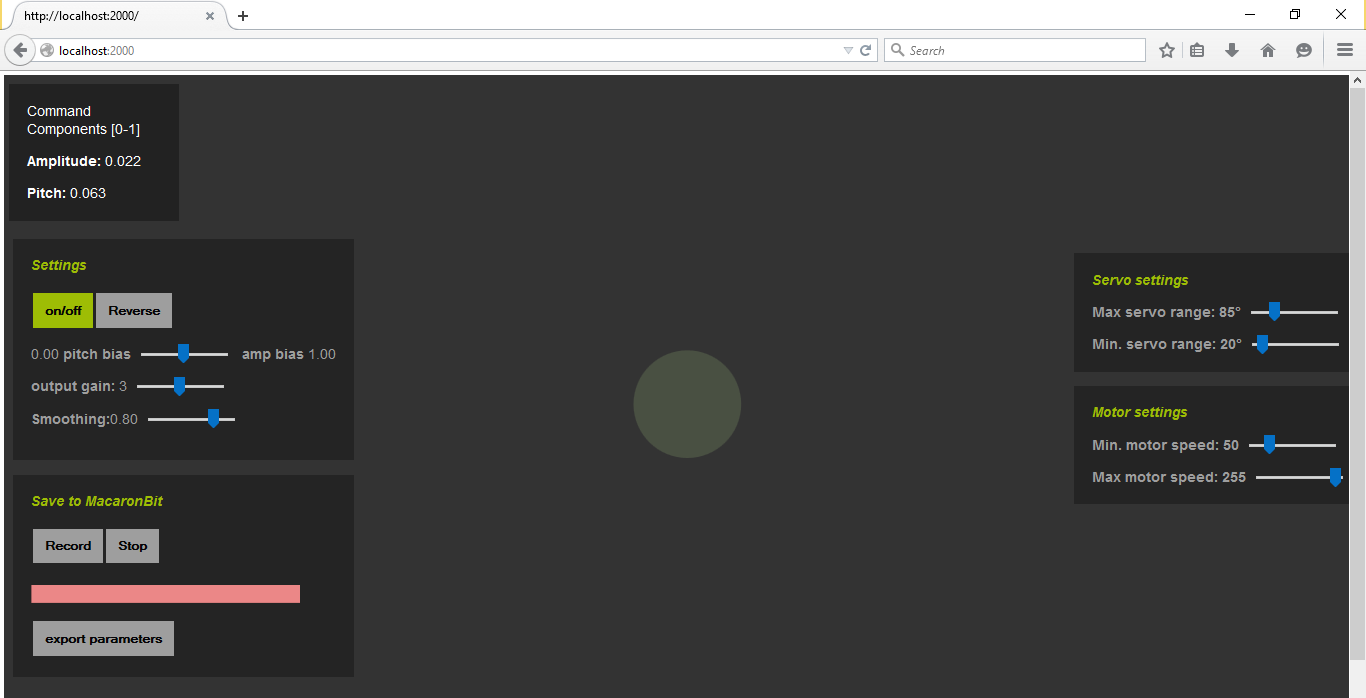
\includegraphics[width=\textwidth]{cuddlebit/VoodleScreenshot} 
	      \caption{Voodle, a vocal doodling interface that uses voice to control the CuddleBit. The circle in the middle visualizes the CuddleBit's movement on-screen, while  additional controls adjust algorithms for vocal processing.}
	      \label{fig:voodle}
   \end{subfigure}
   \qquad
   \begin{subfigure}{\textwidth}
   	   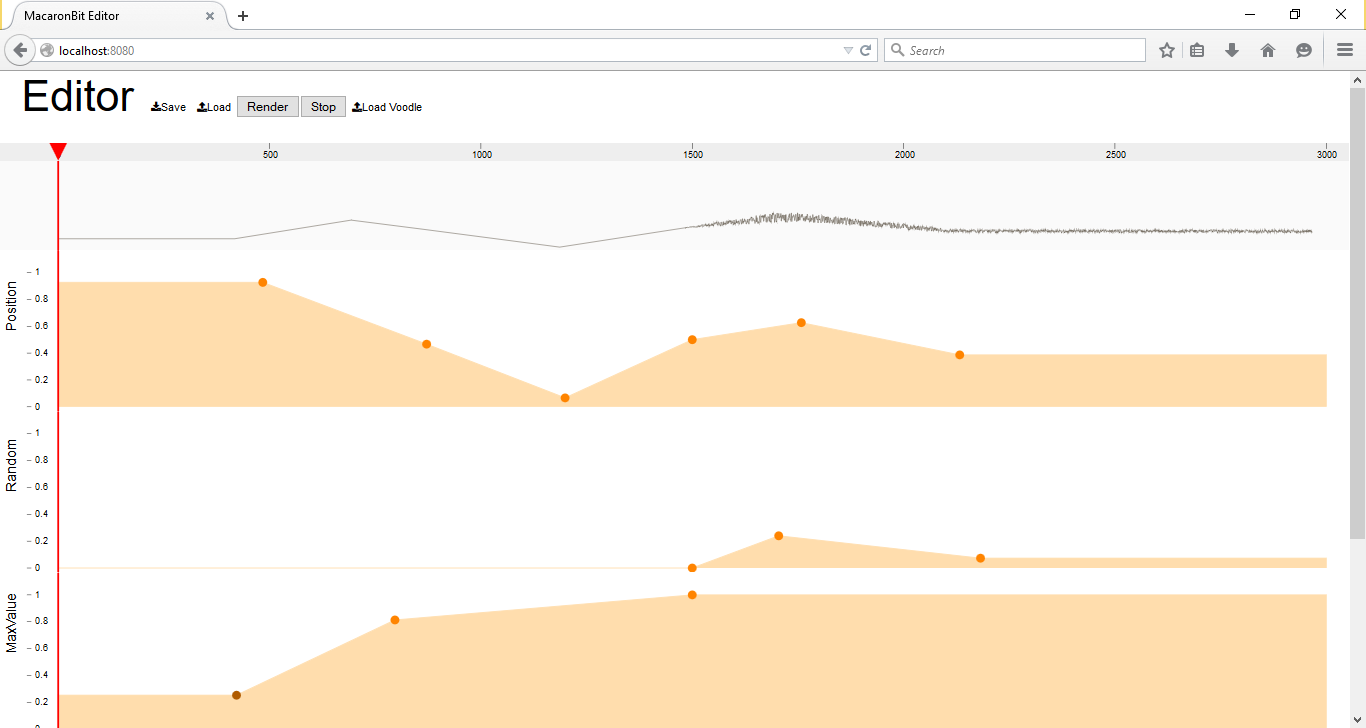
\includegraphics[width=\textwidth]{cuddlebit/MacaronBitScreenshot} 
	      \caption{MacaronBit, a version of Macaron (\autoref{ch:macaron}) extended to control CuddleBits.}
	      \label{fig:macaronbit}
   \end{subfigure}
   \caption{CuddleBit design tools. Voodle enables initial \emph{sketching} of affective robot behaviours, while MacaronBit enables \emph{refining}.}
   \label{fig:cuddlebitdesigntools}
\end{figure}

Voodle (\autoref{fig:voodle}), from ``vocal doodling", is a novel sketching interface to easily create 1-DoF behaviours using non-speech voice, in particular, ideophones \cite{Dingemanse2012} like ``Ooooh" and ``Bwooop."
It is inspired by the onomatopoeia descriptions found with our initial exploration (\autoref{ch:hapticinstrument}) and previous work \cite{Seifi2015,Watanabe2012}.
Through a series of user studies, we developed a prioritized set of ideophones and how they mapped to movements of the CuddleBit.
At the time of writing, Voodle is in active development; we are using participatory design to further identify critical features, Voodle's expressive capability, and how it might fit into a design tool suite for the CuddleBit alongside Macaron.

MacaronBit (\autoref{fig:macaronbit}) is an adaptation of Macaron (\autoref{ch:macaron}) to control 1-DoF CuddleBit using a familiar track-based metaphor.
Instead of two tracks controlling amplitude and frequency, MacaronBit has five: low-frequency amplitude and frequency (for breathing); high-frequency amplitude and frequency (for ``shakiness" or ``noise"), and bias (asymmetry in the signal), determined during piloting.

Voodle and MacaronBit are symbiotic.
Users can record voodles and export them to MacaronBit; initial result suggest that they each support different goals for users.
Together, Voodle and MacaronBit represent sketching (\autoref{ch:hapticinstrument}) and refining (\autoref{ch:tactileanimation}, showing that this dichotomy provides a useful framing when creating \haxd support tools and applies to other display types beyond VT icon design.
Research is ongoing in a series of user studies, exploring expressiveness and consistency of designed behaviours, the specific capabilities and roles of the two tools, and important considerations for future development.


\endinput
